\documentclass{article}
\usepackage{iclr2027_conference,times}
\usepackage[UTF8]{ctex}
\usepackage{amsmath,amssymb,mathtools}
\usepackage{booktabs}
\usepackage{longtable}
\usepackage{graphicx}
\usepackage{flafter}
\usepackage{float}
\usepackage{placeins}
\usepackage{microtype}
\usepackage{xcolor}
\usepackage{colortbl}
\usepackage{hyperref}
\usepackage{url}

\definecolor{tabblue}{RGB}{76,114,176}
\definecolor{taborange}{RGB}{221,132,82}
\definecolor{tabgreen}{RGB}{85,168,104}
\definecolor{tabred}{RGB}{196,78,82}
\definecolor{tabpurple}{RGB}{129,114,179}
\definecolor{tabgray}{RGB}{110,110,110}
\definecolor{lightgray}{gray}{0.93}

% Shared notation for the arXiv and conference entry points.
\newcommand{\method}{TabACE}
\newcommand{\methodlong}{Tabular Adaptive Context Ensemble}
\newcommand{\methodmath}{\mathrm{TabACE}}
\newcommand{\dataset}{\mathcal{D}}
\newcommand{\model}{\mathcal{M}_{\theta}}
\newcommand{\contextset}{\mathcal{C}}

% Shared theorem environments for the main theoretical analysis.
\newtheorem{proposition}{Proposition}[section]
\newtheorem{lemma}[proposition]{Lemma}
\newtheorem{theorem}{Theorem}

% Lightweight shared algorithm float; the full algorithm packages are not
% required by either manuscript entry point.
\floatstyle{ruled}
\newfloat{algorithm}{tbp}{loa}
\floatname{algorithm}{Algorithm}

% Keep unfinished material conspicuous in working PDFs.  The arXiv package
% target refuses to run while any \TODO commands remain in the manuscript.
\newcommand{\TODO}[1]{\textcolor{red}{[TODO: #1]}}

\newcommand{\ICLRLayout}{}
\hypersetup{hidelinks}
\renewenvironment{abstract}
  {\vskip.075in\centerline{\large\bfseries 摘要}\vspace{0.5ex}\begin{quote}}
  {\par\end{quote}\vskip 1ex}

\title{TabACE：通过自适应上下文集成实现表格基础模型的鲁棒推理}
\author{匿名作者}
\renewcommand{\refname}{参考文献}

\begin{document}
\maketitle

\begin{abstract}
表格基础模型（Tabular Foundation Models，TFMs）凭借上下文学习能力，在各类预测任务中展现出优异性能。然而，上下文一旦受到扰动或发生偏移，同一查询样本的预测便可能大幅波动。利用 TFM 上下文的可配置性，我们提出 \textbf{\method{}}（Adaptive Context Ensembling），一种模型无关、无需训练的推理策略，用于增强预测稳健性。\method{} 聚合由不同替代上下文得到的预测，并且仅当这些预测具有充分一致性且任务特定门控支持更新时，才修改默认预测（Base）。我们给出理论风险界，说明该聚合与整合机制能够有效限制有害更新。在涵盖五种上下文扰动和七种分布偏移的 OpenML 基准、全合成设置以及自然分布偏移上，\method{} 在保持干净数据性能的同时，持续缓解基础模型和常规预测器的性能退化。此外，通过缓存可复用的上下文计算，重复推理可获得近六倍加速。

\end{abstract}

\section{引言}
\label{sec:introduction}

对于一个冻结的 TFM，每次预测都同时依赖查询样本和带标签上下文。TFM 在多个任务上进行预训练，并通过上下文学习对查询样本进行预测，而无需更新数据集特定参数
\citep{muller2023tabpfn,hollmann2025tabpfn,qu2025tabicl,ma2025tabdpt}。
这类模型可用于医疗、金融、科学与工业领域的分类和回归任务。即使模型和查询样本保持不变，改变上下文样本、特征或标签仍可能改变预测结果 \citep{abdullah2026contextsampling}。因此，模型的稳健性不仅取决于查询数据，也取决于上下文的使用方式。

一个任务可以通过压缩、检索、样本选择、特征或响应变换以及分布对齐等方式构造多种上下文
\citep{feuer2024tunetables,thomas2024localpfn,xu2025mixturepfn,
treerath2026tabaicl,hollmann2025tabpfn,khalifa2023dense}。这些构造在不同变化下能够提供互补证据，但不存在一种构造可以在所有变化下始终可靠。我们将冻结预测器在原始、未经修改的上下文上得到的输出称为 \emph{Base}。直接平均相互冲突的替代预测，可能使原本准确的 Base 预测变差。因此，需要一种查询级机制来判断这些替代预测是否为更新提供了足够一致的证据，并在证据较弱时将输出锚定到 Base。

\textbf{\method{}} 将这一决策实现为无需额外训练主干模型的查询自适应上下文集成。该方法保留原始上下文作为 Base，并通过样本组成、特征与响应视图以及分布对齐构造互补上下文。同一个冻结预测器通过统一的输出接口评估每个上下文。置信度与跨上下文一致性共同决定替代预测的聚合结果，任务特定门控则控制更新幅度：支持证据越强，聚合结果的影响越大；支持证据较弱时，预测仍锚定到 Base。上下文构造和预测融合均不使用真实目标标签。\method{}-shared 在预定义变化上采用固定上下文库，且不接收变化类别或强度；若推理前已知变化类别，\method{}-specific 会加入相应候选上下文，但仍不接收变化强度。该接口无需改变模型架构，便可迁移到 TabPFN、TabICL、TabDPT 和 LimiX 等不同 TFM。

我们在 OpenML 任务、全合成数据与自然分布偏移上评估 \method{}，覆盖五种受控上下文扰动和七种分布偏移。在四个冻结的 TFM（LimiX-2M、TabICL-v2、TabPFN-v3 和 TabDPT v1.2）上，\method{}-shared 在所有非零强度的 OpenML 扰动与偏移指标上均优于 Base，同时保持接近的干净数据得分。在 180 个对齐的合成实验单元上，该方法的平均成对稳定性胜率排名第一，分类和回归分别达到 $67.0\%$ 和 $87.6\%$。在给定变化类别先验时，\method{}-specific 进一步提升性能；同一接口也适用于常规预测器。这些结果表明，可配置上下文能够在无需重新训练的情况下提高推理时稳健性。
\FloatBarrier

\section{相关工作}
\label{sec:related}

\noindent\textbf{表格基础模型的上下文敏感性。}
表格基础模型通过以带标签样本行为条件，对无标签查询样本进行预测。TabPFN 奠定了基于合成先验的推理范式，TabICL 将表格上下文学习扩展到更大规模的数据集，TabDPT 则将检索机制与真实数据预训练相结合~\citep{muller2023tabpfn,qu2025tabicl,ma2025tabdpt}。后续工作进一步扩展了预训练规模、可扩展性与任务覆盖范围~\citep{hollmann2025tabpfn,grinsztajn2025tabpfn25,qu2026tabiclv2}。有关上下文采样的研究还表明，上下文的规模、覆盖范围与采样方式都会影响预测准确性和稳定性~\citep{abdullah2026contextsampling}。这些工作改进了模型设计和规模，但并未在冻结模型下对不同构造方式产生的上下文预测进行组合。

\medskip
\noindent\textbf{上下文压缩、检索与选择。}
TuneTables、LoCalPFN、MixturePFN 和 Tab-AICL 分别通过压缩、检索、路由或主动获取来构造推理上下文~\citep{feuer2024tunetables,thomas2024localpfn,xu2025mixturepfn,
treerath2026tabaicl}。\method{} 将上下文选择扩展为上下文集成：上述方法通常优化或选择一个主导上下文或专家，以提高可扩展性或查询相关性；而 \method{} 则整合由异质上下文构造器诱导的预测。

\medskip
\noindent\textbf{上下文集成与构造多样性。}
在表格学习之外，已有上下文集成方法会组合由不同示例子集得到的预测；例如，DENSE 对这些预测进行平均~\citep{khalifa2023dense}。在表格预测中，TabPFN 会集成不同预处理方式以及特征或标签置换得到的变体~\citep{hollmann2025tabpfn}。\method{} 将上下文集成从同一构造方案的多个变体扩展到具有不同归纳偏置的异质构造器，并依据查询级证据分配其影响。

\begin{figure}[!t]
  \centering
  \ifdefined\ICLRLayout
    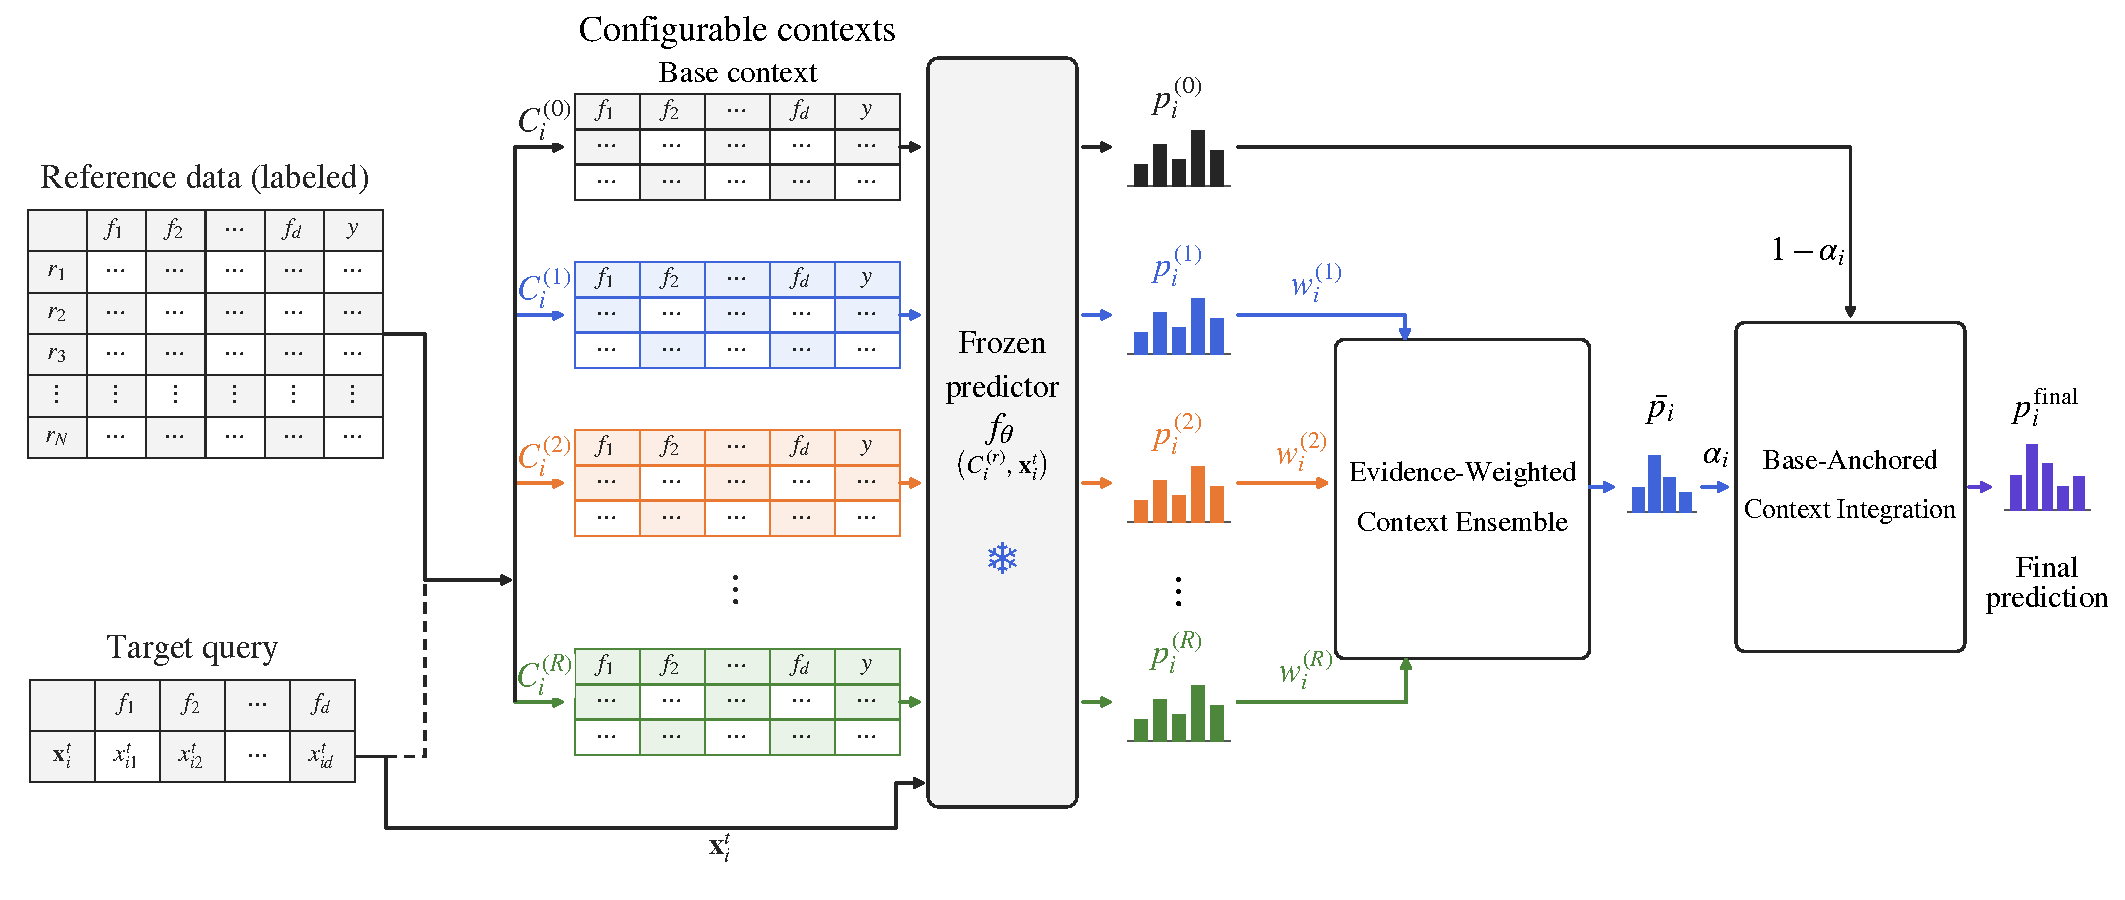
\includegraphics[width=\textwidth]{figures/context_ensemble_framework_pfn_input_semantics_fixed_lines.pdf}
  \else
    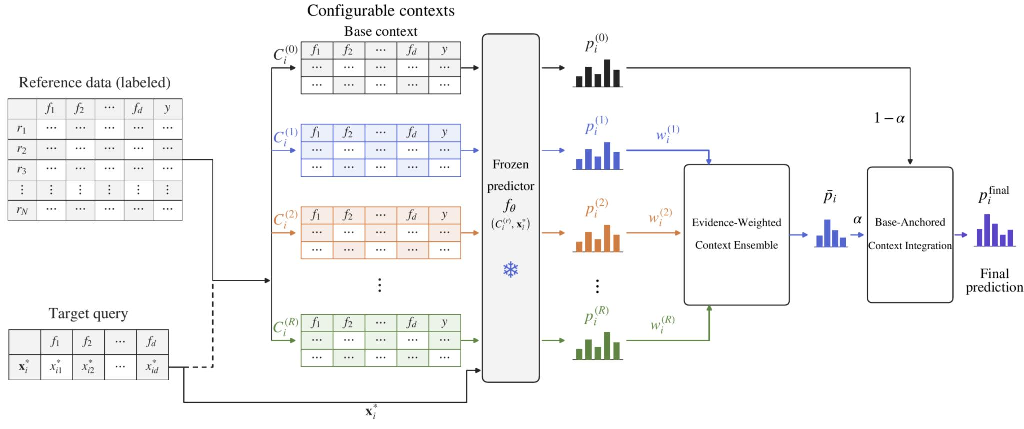
\includegraphics[width=0.86\textwidth]{figures/adaptive_context_ensemble_framework.pdf}
  \fi
  \caption{\textbf{\method{} 的框架概览。}
  对每个查询样本，冻结预测器分别评估 Base 与可配置构造器产生的替代上下文。置信度和一致性决定各替代预测的权重，查询相关门控再将其聚合结果与 Base 融合。图中的 $p_i^{(r)}$ 表示分类概率向量；回归任务在同一流程中使用标量预测 $\hat y_i^{(r)}$。}
  \label{fig:tabace_overview}
\end{figure}

\medskip
\noindent\textbf{常规条件与偏移条件下的上下文变化。}
已有研究在多种数据变化条件下考察了表格预测的稳健性。经典标签偏移方法估计或重新校准目标类别先验~\citep{lipton2018bbse,alexandari2020labelshift}；DistPFN、Drift-Resilient TabPFN 和 SPN 则分别处理表格上下文学习中的标签偏移、时间偏移与策略性偏移~\citep{lee2026distpfn,helli2024drifttabpfn,
lv2026strategic}。SkillTFM 通过按证据检索外部修复技能来适配冻结的 TFM；其运行时证书决定是否采用修复，否则回退到基础预测器~\citep{he2026skilltfm}。TableShift 与 TabFSBench 分别提供分布偏移表格任务和受控特征变化的基准~\citep{gardner2023tableshift,
cheng2025tabfsbench}。上下文采样研究还表明，即便在常规评估条件下，上下文选择也会影响 TFM 预测~\citep{abdullah2026contextsampling}。因此，我们同时在常规变化与多种受控变化类别下研究上下文聚合。

\section{方法}
\label{sec:method}

\subsection{问题设定与方法概述}

记 $\mathcal D_s=\{(x_j^s,y_j^s)\}_{j=1}^{n_s}$ 为带标签参考数据，$\mathcal X_t=\{x_i^t\}_{i=1}^{n_t}$ 为无标签目标批次，其中的样本即目标查询。分类任务的输出空间为 $\mathcal Y=\{1,\ldots,L\}$，回归任务的输出空间为 $\mathcal Y\subseteq\mathbb R$。冻结的表格基础模型 $f_\theta$ 根据一个带标签上下文对每个查询样本进行预测。该上下文由源样本构造；对于已注册的选择偏移构造器，还可包含带伪标签的目标样本。真实目标标签仅用于评估，测试时始终不更新 $f_\theta$。参考样本与目标样本分别服从 $P_s(X,Y)$ 和 $P_t(X,Y)$。我们既研究可访问上下文的受控变化，也研究满足 $P_t\neq P_s$ 的分布偏移；推理时仅使用 $\mathcal D_s$ 与 $\mathcal X_t$。

如图~\ref{fig:tabace_overview} 所示，\method{} 在保持 $f_\theta$ 冻结的同时，使用一个 Base 分支和多个替代上下文分支。置信度与跨上下文一致性决定各替代分支的相对影响，任务特定门控和总体上下文支持度则决定相对于 Base 的更新幅度。因此，更新由当前查询样本可获得的证据决定。

\subsection{可配置上下文与输出接口}
\label{sec:context_interface}

记 $\Phi=\{\phi_0,\ldots,\phi_R\}$ 为目标推理前根据源侧信息与应用知识选定的分支配置，并以 $\mathcal I(\Phi)=\{r:\phi_r\in\Phi,\ r\geq1\}=\{1,\ldots,R\}$ 表示替代分支的索引集合。$F_{\phi_r}$ 表示由配置 $\phi_r$ 诱导的完整预测映射，而不是另一个额外训练的模型。对于目标批次中的查询样本 $x_i^t$，有
\begin{equation}
  o_i^{(r)}
  =F_{\phi_r}(\mathcal D_s,\mathcal X_t,x_i^t;f_\theta),
  \qquad r=0,\ldots,R.
  \label{eq:context_prediction}
\end{equation}
对于 TFM 分支，该映射将可配置上下文构造器与冻结预测器组合起来。批次共享构造器只需构造一次 $C^{(r)}=G_{\phi_r}(\mathcal D_s,\mathcal X_t)$，随后在不同查询间复用，因此
$F_{\phi_r}(\mathcal D_s,\mathcal X_t,x_i^t;f_\theta)=f_\theta(C^{(r)},x_i^t)$。留一目标构造则生成 $C_i^{(r)}=G_{\phi_r}(\mathcal D_s,\mathcal X_t,x_i^t)$。对于兼容的常规预测器，所构造的上下文充当该分支的训练数据，并暴露相同的输出接口。分类任务中，$o_i^{(r)}=p_i^{(r)}\in\Delta^{L-1}$ 为类别概率向量；点回归任务中，$o_i^{(r)}=\hat y_i^{(r)}$ 为标量。

我们将 $\phi_0$ 保留给 Base 分支，并以 $o_i^{(0)}$ 表示其输出。其构造器 $G_{\phi_0}$ 遵循主干模型的标准采样规则，从可用的带标签参考数据中形成规范上下文，不依据目标数据修改所选特征或标签。对于 $r\geq1$，$G_{\phi_r}$ 通过选择或重加权参考样本、选择或变换特征，或者应用预先规定且由源数据确定的标签调整来构造互补上下文。选择偏移构造器还可将 Base 伪标签附加到目标样本行上。对于查询 $x_i^t$，这些样本行为
$\widehat{\mathcal D}_{t,-i}^{(0)}=\{(x_j^t,\widetilde y_j^{(0)}):j\neq i\}$，其中 $\widetilde y_j^{(0)}=\arg\max_{\ell\in\mathcal Y}p_{j,\ell}^{(0)}$。因此，当前查询样本不会被放入自身的上下文。上述操作可依赖参考特征、参考标签以及无标签目标批次的统计量；留一构造还依赖当前查询样本，但任何构造都不使用目标标签。当构造器选择特征子集时，同一投影会同时作用于上下文和查询样本。由这些配置得到替代输出库
\begin{equation}
  \mathcal O_i(\Phi)=\{o_i^{(r)}:r\in\mathcal I(\Phi)\}.
  \label{eq:output_bank}
\end{equation}
其中，$\Phi$ 指定上下文构造规则，$\mathcal O_i(\Phi)$ 汇集这些规则针对查询样本产生的输出。

\subsection{基于置信度与一致性的上下文聚合}
\label{sec:evidence_aggregation}

对于查询样本 $x_i^t$，$R$ 个替代上下文产生式~\eqref{eq:output_bank} 中的输出。我们先分别为分类和回归构造与任务兼容的支持度得分，再使用统一的归一化加权规则聚合相应预测。

在分类任务中，令 $p_i^{(r)}\in\Delta^{L-1}$ 为上下文 $r$ 的预测。给定从源数据学习的非负系数 $\eta_{Q,r},\eta_{S,r}\geq0$，计算
\begin{equation}
  \begin{aligned}
    \mu_i&=\frac{1}{R}\sum_{s=1}^{R}p_i^{(s)},
    &Q_i^{(r)}&=1-\frac{H(p_i^{(r)})}{\log L},\\
    S_i^{(r)}&=1-\frac12\lVert p_i^{(r)}-\mu_i\rVert_1,
    &\rho_i^{(r)}&=\eta_{Q,r}Q_i^{(r)}+\eta_{S,r}S_i^{(r)}.
  \end{aligned}
  \label{eq:classification_evidence}
\end{equation}
其中 $H(p)=-\sum_{\ell=1}^{L}p_\ell\log p_\ell$。$Q_i^{(r)}$ 衡量归一化熵置信度，$S_i^{(r)}$ 衡量该预测与替代预测均值的一致性；二者同时较高时，$\rho_i^{(r)}$ 增大。

在回归任务中，令 $\hat y_i^{(r)}\in\mathbb R$ 为上下文 $r$ 的预测。定义
\begin{equation}
  \begin{aligned}
    m_i&=\operatorname{median}\{\hat y_i^{(s)}\}_{s=1}^{R},
    &S_i^{(r)}&=\exp\!\left(-\frac{|\hat y_i^{(r)}-m_i|}{\tau_y}\right),\\
    \rho_i^{(r)}&=\eta_{S,r}^{\mathrm{reg}}S_i^{(r)},
    \qquad \eta_{S,r}^{\mathrm{reg}}\geq0.
  \end{aligned}
  \label{eq:regression_evidence}
\end{equation}
中位数 $m_i$ 是稳健中心，$\tau_y>0$ 由源数据确定；偏离该中心较远的预测获得较低支持度。

两个任务随后采用相同的归一化加权与聚合规则：
\begin{equation}
  \begin{aligned}
    w_i^{(r)}&=\frac{\pi_r e^{\rho_i^{(r)}}}
      {\sum_{s=1}^{R}\pi_s e^{\rho_i^{(s)}}},\\
    \bar o_i&=\sum_{r=1}^{R}w_i^{(r)}o_i^{(r)},
    \qquad \sum_{r=1}^{R}w_i^{(r)}=1.
  \end{aligned}
  \label{eq:task_aware_aggregation}
\end{equation}
其中 $\pi_r>0$ 是从源数据学习的上下文 $r$ 的先验可靠性，并满足 $\sum_r\pi_r=1$。分类任务取 $o_i^{(r)}=p_i^{(r)}$，回归任务取 $o_i^{(r)}=\hat y_i^{(r)}$。聚合结果 $\bar o_i$ 随后与 Base 进行整合。

\subsection{与 Base 的查询相关整合}
\label{sec:base_integration}

我们使用任务特定门控 $U_i$ 和总体上下文支持度 $E_i$ 将 $\bar o_i$ 与 Base 整合。分类任务中，$U_i$ 表示 Base 的内在不确定性；回归任务中，$U_i$ 表示 Base 与聚合结果之间的外在差异。相应的 $E_i$ 衡量替代预测的支持度：
\begin{equation}
  \begin{aligned}
    U_i^{\mathrm{cls}}&=\frac{H(p_i^{(0)})}{\log L},
    &E_i^{\mathrm{cls}}&=\sum_{r=1}^{R}w_i^{(r)}Q_i^{(r)}S_i^{(r)},\\
    U_i^{\mathrm{reg}}&=1-\exp\!\left(-\frac{|\bar y_i-\hat y_i^{(0)}|}{\tau_y}\right),
    &E_i^{\mathrm{reg}}&=\sum_{r=1}^{R}w_i^{(r)}S_i^{(r)}.
  \end{aligned}
  \label{eq:context_integration_evidence}
\end{equation}
下文以 $U_i$ 和 $E_i$ 表示当前任务对应的这一对量。

两个任务采用相同的整合规则：
\begin{equation}
  \alpha_i=\alpha_{\max}U_iE_i,
  \qquad o_i^{\mathrm{final}}
  =(1-\alpha_i)o_i^{(0)}+\alpha_i\bar o_i.
  \label{eq:base_anchored_update}
\end{equation}
由于 $U_i$、$E_i$ 和 $\alpha_{\max}$ 均位于 $[0,1]$，$\alpha_i$ 也位于该区间。因此，只要任务特定门控或上下文支持度较弱，更新就会锚定到 Base。

\paragraph{外层折策略学习。}
我们在外层训练数据集生成的校准 episode 上拟合上下文先验、得分系数、输出尺度与整合上限。每个 episode 将一个带标签源上下文与一个伪目标批次配对；构造器可以访问该批次的特征，而其标签仅进入校准损失。在留出数据推理之前，拟合后的策略与 $\Phi$ 均保持固定。

\ifdefined\ICLRLayout\clearpage\fi
\subsection{理论分析}
\label{sec:theory}

本节给出上下文聚合优于 Base 的充分条件，并刻画任务门控融合如何根据上下文支持度控制预测变化。令 $g_0$ 与 $g_{\mathrm{final}}$ 分别输出 $o_i^{(0)}$ 与 $o_i^{\mathrm{final}}$，并定义 $\mathcal R_t(g)=\mathbb E_{(x,y)\sim P_t}[\ell(g(x),y)]$。对于关于预测参数凸的损失函数 $\ell$，上下文 $r$ 以及上下文聚合结果相对于 Base 的改进分别定义为
\begin{equation}
  \Delta_i^{(r)}
  =\ell(o_i^{(0)},y_i^t)-\ell(o_i^{(r)},y_i^t),
  \qquad
  \Delta_i
  =\ell(o_i^{(0)},y_i^t)-\ell(\bar o_i,y_i^t).
  \label{eq:context_improvements}
\end{equation}
这些量只在理论分析中使用目标标签；上下文构造、支持度评分与预测均不使用目标标签。

\paragraph{互补上下文覆盖。}
对于变化类别 $h$，不同替代上下文会在不同查询子集上改进 Base。以 $C_h(\Phi)$ 表示目标分布下，上下文库 $\Phi$ 中至少一个上下文相对 Base 改进不少于 $\delta_+$ 的概率。若一个新上下文增加了现有上下文库尚未覆盖的有益查询，则称其具有互补性。形式化定义与收益递减性质见附录~\ref{app:repair-coverage}。

\begin{theorem}[加权上下文聚合的风险界]
\label{thm:effective_context_repair}
对于查询 $i$ 和固定上下文库 $\Phi$，假设存在非空有效集合 $\mathcal G_i$，使得对于某些 $\delta_+>0$、$\delta_-\geq0$ 和 $\rho_+>\rho_-$，有
\begin{equation}
\begin{aligned}
\Delta_i^{(r)}&\geq\delta_+,&\rho_i^{(r)}(\Phi)&\geq\rho_+&& (r\in\mathcal G_i),\\
\Delta_i^{(r)}&\geq-\delta_-,&\rho_i^{(r)}(\Phi)&\leq\rho_-&& (r\in\mathcal I(\Phi)\setminus\mathcal G_i).
\end{aligned}
\label{eq:repair_conditions}
\end{equation}
令 $\Pi_i=\sum_{r\in\mathcal G_i}\pi_r$，$W_i=\sum_{r\in\mathcal G_i}w_i^{(r)}$，则
\begin{equation}
\begin{aligned}
W_i&\geq\underline W_i
=\left[1+\frac{1-\Pi_i}{\Pi_i}
e^{-(\rho_+-\rho_-)}\right]^{-1},\\
\Delta_i&\geq\gamma_i
:=\underline W_i\delta_+-(1-\underline W_i)\delta_-.
\end{aligned}
\label{eq:repair_margin}
\end{equation}
因此，$\underline W_i>\delta_-/(\delta_++\delta_-)$ 蕴含 $\gamma_i>0$，且
\begin{equation}
  \ell(o_i^{\mathrm{final}},y_i^t)-\ell(o_i^{(0)},y_i^t)
  \leq-\alpha_i\Delta_i
  \leq-\alpha_{\max}U_iE_i\gamma_i.
  \label{eq:query_repair_gain}
\end{equation}

令 $\mathcal A_\Phi$ 包含满足上述分离条件且 $\gamma_i>0$ 的查询，则目标风险之差满足
\begin{equation}
  \mathcal R_t(g_{\mathrm{final}})-\mathcal R_t(g_0)
  \leq-\Gamma_t(\Phi)+\varepsilon_t(\Phi),
  \label{eq:changed_risk_gain}
\end{equation}
其中
\begin{equation}
\begin{aligned}
\Gamma_t(\Phi)
&:=\alpha_{\max}\mathbb E_{P_t}
  [U_iE_i\gamma_i\mathbf 1\{i\in\mathcal A_\Phi\}],\\
\varepsilon_t(\Phi)
&:=\alpha_{\max}\mathbb E_{P_t}
  [U_iE_i(-\Delta_i)_+\mathbf 1\{i\notin\mathcal A_\Phi\}].
\end{aligned}
\label{eq:repair_residual_terms}
\end{equation}
因此，$\Gamma_t(\Phi)>\varepsilon_t(\Phi)$ 蕴含 $\mathcal R_t(g_{\mathrm{final}})<\mathcal R_t(g_0)$。
\end{theorem}

\paragraph{证明概述。}
得分分离条件给出有效集合 $\mathcal G_i$ 的归一化权重下界 $W_i\geq\underline W_i$。随后利用凸性将该权重界转化为聚合改进 $\gamma_i$，进而得到式~\eqref{eq:query_repair_gain} 的查询级收益。将目标分布期望分别限制在 $\mathcal A_\Phi$ 及其补集上，即可得到式~\eqref{eq:changed_risk_gain}。完整证明见附录~\ref{app:theorem-proof}。

\paragraph{推论。}
更大的有效先验质量 $\Pi_i$ 或更宽的得分间隔 $\rho_+-\rho_-$ 会提高 $\underline W_i$，从而增大有保证的聚合收益 $\gamma_i$。互补上下文决定潜在有益覆盖范围，得分加权与门控则决定该覆盖如何转化为实际风险变化。以下恒等式精确给出各任务特定更新相对于 Base 的幅度：
\begin{equation}
  \lVert o_i^{\mathrm{final}}-o_i^{(0)}\rVert
  =\alpha_{\max}U_iE_i
   \lVert\bar o_i-o_i^{(0)}\rVert.
  \label{eq:base_preservation_identity}
\end{equation}
因此，当 $U_iE_i=0$ 时，预测恢复为 Base。分类与回归的任务特定界见附录~\ref{app:theory}。

\ifdefined\ICLRLayout
\clearpage
% 中文版保留原始数值与方法名称。
\definecolor{tabaceSharedRow}{HTML}{EAF4FB}
\definecolor{tabaceSpecificRow}{HTML}{FFF4D6}
\definecolor{tabaceSharedText}{HTML}{0072B2}
\definecolor{tabaceSpecificText}{HTML}{D55E00}
\ifdefined\ICLRLayout
\begin{table}[H]
\else
\begin{table}[H]
\fi
  \caption{OpenML-CC18 分类与 OpenML-CTR23 回归任务上的整体性能。扰动和偏移区块分别在五种和七种变化类别的全部非零强度上进行宏平均。}
  \label{tab:overall-performance}
  \centering
  \scriptsize
  \setlength{\tabcolsep}{2.0pt}
  \renewcommand{\arraystretch}{0.98}
  \begin{tabular}{@{}l*{12}{c}@{}}
    \toprule
    & \multicolumn{4}{c}{干净数据}
    & \multicolumn{4}{c}{五种扰动（平均）}
    & \multicolumn{4}{c}{七种偏移（平均）} \\
    \cmidrule(lr){2-5}\cmidrule(lr){6-9}\cmidrule(lr){10-13}
    & \multicolumn{2}{c}{分类} & \multicolumn{2}{c}{回归}
    & \multicolumn{2}{c}{分类} & \multicolumn{2}{c}{回归}
    & \multicolumn{2}{c}{分类} & \multicolumn{2}{c}{回归} \\
    \cmidrule(lr){2-3}\cmidrule(lr){4-5}
    \cmidrule(lr){6-7}\cmidrule(lr){8-9}
    \cmidrule(lr){10-11}\cmidrule(lr){12-13}
    方法
    & Acc$\uparrow$ & AUC$\uparrow$ & $R^2\uparrow$ & nRMSE$\downarrow$
    & Acc$\uparrow$ & AUC$\uparrow$ & $R^2\uparrow$ & nRMSE$\downarrow$
    & Acc$\uparrow$ & AUC$\uparrow$ & $R^2\uparrow$ & nRMSE$\downarrow$ \\
    \midrule
    \multicolumn{13}{@{}l}{\textit{非 TFM 基线}} \\
    LogReg/Ridge + HPO & 0.754 & 0.867 & 0.543 & 0.684 & 0.418 & 0.582 & -0.559 & 1.175 & 0.719 & 0.775 & -0.490 & 0.851 \\
    SVM/SVR + HPO & 0.777 & 0.879 & 0.492 & 0.703 & 0.449 & 0.611 & -0.872 & 1.255 & 0.757 & 0.793 & 0.010 & 0.873 \\
    kNN + HPO & 0.726 & 0.856 & 0.587 & 0.656 & 0.489 & 0.647 & -1.245 & 1.396 & 0.743 & 0.775 & 0.327 & 0.779 \\
    RF + HPO & 0.776 & 0.886 & 0.676 & 0.561 & 0.451 & 0.649 & -1.218 & 1.335 & 0.760 & 0.810 & 0.385 & 0.724 \\
    LightGBM + HPO & 0.776 & 0.884 & 0.697 & 0.529 & 0.463 & 0.639 & -1.215 & 1.337 & 0.759 & 0.796 & 0.350 & 0.736 \\
    CatBoost + HPO & 0.782 & 0.890 & 0.708 & 0.514 & 0.479 & 0.653 & -1.372 & 1.368 & 0.770 & 0.811 & 0.381 & 0.711 \\
    XGBoost + HPO & 0.774 & 0.885 & 0.702 & 0.525 & 0.455 & 0.640 & -1.323 & 1.359 & 0.751 & 0.796 & 0.278 & 0.767 \\
    MLP + HPO & 0.729 & 0.858 & 0.583 & 0.568 & 0.435 & 0.604 & -1.007 & 1.272 & 0.741 & 0.767 & 0.066 & 0.828 \\
    FT-Transformer & 0.745 & 0.861 & 0.657 & 0.568 & 0.456 & 0.619 & -1.256 & 1.353 & 0.716 & 0.765 & 0.210 & 0.822 \\
    TabM & 0.735 & 0.866 & 0.655 & 0.577 & 0.454 & 0.614 & -1.100 & 1.324 & 0.699 & 0.743 & 0.212 & 0.811 \\
    TabulaRNN & 0.722 & 0.856 & 0.580 & 0.648 & 0.454 & 0.625 & -0.851 & 1.270 & 0.718 & 0.754 & 0.205 & 0.845 \\
    MambaTab & 0.748 & 0.869 & 0.663 & 0.564 & 0.434 & 0.602 & -0.824 & 1.230 & 0.751 & 0.784 & 0.279 & 0.761 \\
    RealMLP & 0.762 & 0.872 & 0.694 & 0.527 & 0.448 & 0.614 & -1.258 & 1.326 & 0.758 & 0.793 & 0.240 & 0.749 \\
    \midrule
    LimiX-2M & 0.796 & 0.896 & 0.724 & 0.494 & 0.475 & 0.657 & -1.141 & 1.277 & 0.781 & 0.831 & 0.385 & 0.689 \\
    \rowcolor{tabaceSharedRow}
    \textcolor{tabaceSharedText}{\textbf{+ \method{}-shared}} & \textcolor{tabaceSharedText}{\textbf{0.796}} & \textcolor{tabaceSharedText}{\textbf{0.896}} & \textcolor{tabaceSharedText}{\textbf{0.725}} & \textcolor{tabaceSharedText}{\textbf{0.493}} & \textcolor{tabaceSharedText}{\textbf{0.542}} & \textcolor{tabaceSharedText}{\textbf{0.716}} & \textcolor{tabaceSharedText}{\textbf{-0.173}} & \textcolor{tabaceSharedText}{\textbf{1.059}} & \textcolor{tabaceSharedText}{\textbf{0.784}} & \textcolor{tabaceSharedText}{\textbf{0.835}} & \textcolor{tabaceSharedText}{\textbf{0.498}} & \textcolor{tabaceSharedText}{\textbf{0.659}} \\
    \rowcolor{tabaceSpecificRow}
    \textcolor{tabaceSpecificText}{\textbf{+ \method{}-specific}} & \textcolor{tabaceSpecificText}{\textbf{0.796}} & \textcolor{tabaceSpecificText}{\textbf{0.896}} & \textcolor{tabaceSpecificText}{\textbf{0.725}} & \textcolor{tabaceSpecificText}{\textbf{0.493}} & \textcolor{tabaceSpecificText}{\textbf{0.628}} & \textcolor{tabaceSpecificText}{\textbf{0.769}} & \textcolor{tabaceSpecificText}{\textbf{0.053}} & \textcolor{tabaceSpecificText}{\textbf{0.947}} & \textcolor{tabaceSpecificText}{\textbf{0.804}} & \textcolor{tabaceSpecificText}{\textbf{0.847}} & \textcolor{tabaceSpecificText}{\textbf{0.629}} & \textcolor{tabaceSpecificText}{\textbf{0.563}} \\
    \midrule
    TabICL-v2 & 0.804 & 0.901 & 0.739 & 0.476 & 0.494 & 0.676 & -1.077 & 1.270 & 0.763 & 0.826 & 0.273 & 0.730 \\
    \rowcolor{tabaceSharedRow}
    \textcolor{tabaceSharedText}{\textbf{+ \method{}-shared}} & \textcolor{tabaceSharedText}{\textbf{0.804}} & \textcolor{tabaceSharedText}{\textbf{0.901}} & \textcolor{tabaceSharedText}{\textbf{0.738}} & \textcolor{tabaceSharedText}{\textbf{0.478}} & \textcolor{tabaceSharedText}{\textbf{0.575}} & \textcolor{tabaceSharedText}{\textbf{0.720}} & \textcolor{tabaceSharedText}{\textbf{0.363}} & \textcolor{tabaceSharedText}{\textbf{0.783}} & \textcolor{tabaceSharedText}{\textbf{0.772}} & \textcolor{tabaceSharedText}{\textbf{0.831}} & \textcolor{tabaceSharedText}{\textbf{0.467}} & \textcolor{tabaceSharedText}{\textbf{0.659}} \\
    \rowcolor{tabaceSpecificRow}
    \textcolor{tabaceSpecificText}{\textbf{+ \method{}-specific}} & \textcolor{tabaceSpecificText}{\textbf{0.804}} & \textcolor{tabaceSpecificText}{\textbf{0.900}} & \textcolor{tabaceSpecificText}{\textbf{0.738}} & \textcolor{tabaceSpecificText}{\textbf{0.476}} & \textcolor{tabaceSpecificText}{\textbf{0.610}} & \textcolor{tabaceSpecificText}{\textbf{0.752}} & \textcolor{tabaceSpecificText}{\textbf{0.485}} & \textcolor{tabaceSpecificText}{\textbf{0.708}} & \textcolor{tabaceSpecificText}{\textbf{0.805}} & \textcolor{tabaceSpecificText}{\textbf{0.854}} & \textcolor{tabaceSpecificText}{\textbf{0.655}} & \textcolor{tabaceSpecificText}{\textbf{0.535}} \\
    \midrule
    TabPFN-v3 & 0.793 & 0.893 & 0.739 & 0.476 & 0.457 & 0.636 & -1.253 & 1.313 & 0.758 & 0.809 & 0.426 & 0.669 \\
    \rowcolor{tabaceSharedRow}
    \textcolor{tabaceSharedText}{\textbf{+ \method{}-shared}} & \textcolor{tabaceSharedText}{\textbf{0.792}} & \textcolor{tabaceSharedText}{\textbf{0.893}} & \textcolor{tabaceSharedText}{\textbf{0.739}} & \textcolor{tabaceSharedText}{\textbf{0.480}} & \textcolor{tabaceSharedText}{\textbf{0.553}} & \textcolor{tabaceSharedText}{\textbf{0.697}} & \textcolor{tabaceSharedText}{\textbf{0.237}} & \textcolor{tabaceSharedText}{\textbf{0.834}} & \textcolor{tabaceSharedText}{\textbf{0.770}} & \textcolor{tabaceSharedText}{\textbf{0.817}} & \textcolor{tabaceSharedText}{\textbf{0.460}} & \textcolor{tabaceSharedText}{\textbf{0.656}} \\
    \rowcolor{tabaceSpecificRow}
    \textcolor{tabaceSpecificText}{\textbf{+ \method{}-specific}} & \textcolor{tabaceSpecificText}{\textbf{0.792}} & \textcolor{tabaceSpecificText}{\textbf{0.893}} & \textcolor{tabaceSpecificText}{\textbf{0.739}} & \textcolor{tabaceSpecificText}{\textbf{0.477}} & \textcolor{tabaceSpecificText}{\textbf{0.593}} & \textcolor{tabaceSpecificText}{\textbf{0.739}} & \textcolor{tabaceSpecificText}{\textbf{0.588}} & \textcolor{tabaceSpecificText}{\textbf{0.635}} & \textcolor{tabaceSpecificText}{\textbf{0.788}} & \textcolor{tabaceSpecificText}{\textbf{0.835}} & \textcolor{tabaceSpecificText}{\textbf{0.620}} & \textcolor{tabaceSpecificText}{\textbf{0.565}} \\
    \midrule
    TabDPT v1.2 & 0.779 & 0.891 & 0.731 & 0.488 & 0.448 & 0.631 & -1.152 & 1.300 & 0.774 & 0.821 & 0.514 & 0.633 \\
    \rowcolor{tabaceSharedRow}
    \textcolor{tabaceSharedText}{\textbf{+ \method{}-shared}} & \textcolor{tabaceSharedText}{\textbf{0.779}} & \textcolor{tabaceSharedText}{\textbf{0.891}} & \textcolor{tabaceSharedText}{\textbf{0.730}} & \textcolor{tabaceSharedText}{\textbf{0.491}} & \textcolor{tabaceSharedText}{\textbf{0.548}} & \textcolor{tabaceSharedText}{\textbf{0.694}} & \textcolor{tabaceSharedText}{\textbf{0.329}} & \textcolor{tabaceSharedText}{\textbf{0.803}} & \textcolor{tabaceSharedText}{\textbf{0.781}} & \textcolor{tabaceSharedText}{\textbf{0.831}} & \textcolor{tabaceSharedText}{\textbf{0.547}} & \textcolor{tabaceSharedText}{\textbf{0.614}} \\
    \rowcolor{tabaceSpecificRow}
    \textcolor{tabaceSpecificText}{\textbf{+ \method{}-specific}} & \textcolor{tabaceSpecificText}{\textbf{0.779}} & \textcolor{tabaceSpecificText}{\textbf{0.891}} & \textcolor{tabaceSpecificText}{\textbf{0.730}} & \textcolor{tabaceSpecificText}{\textbf{0.488}} & \textcolor{tabaceSpecificText}{\textbf{0.600}} & \textcolor{tabaceSpecificText}{\textbf{0.746}} & \textcolor{tabaceSpecificText}{\textbf{0.443}} & \textcolor{tabaceSpecificText}{\textbf{0.733}} & \textcolor{tabaceSpecificText}{\textbf{0.805}} & \textcolor{tabaceSpecificText}{\textbf{0.846}} & \textcolor{tabaceSpecificText}{\textbf{0.610}} & \textcolor{tabaceSpecificText}{\textbf{0.572}} \\
    \bottomrule
  \end{tabular}
\ifdefined\ICLRLayout
\end{table}
\else
\end{table}
\fi

\else
\begin{figure}[H]
  \centering
  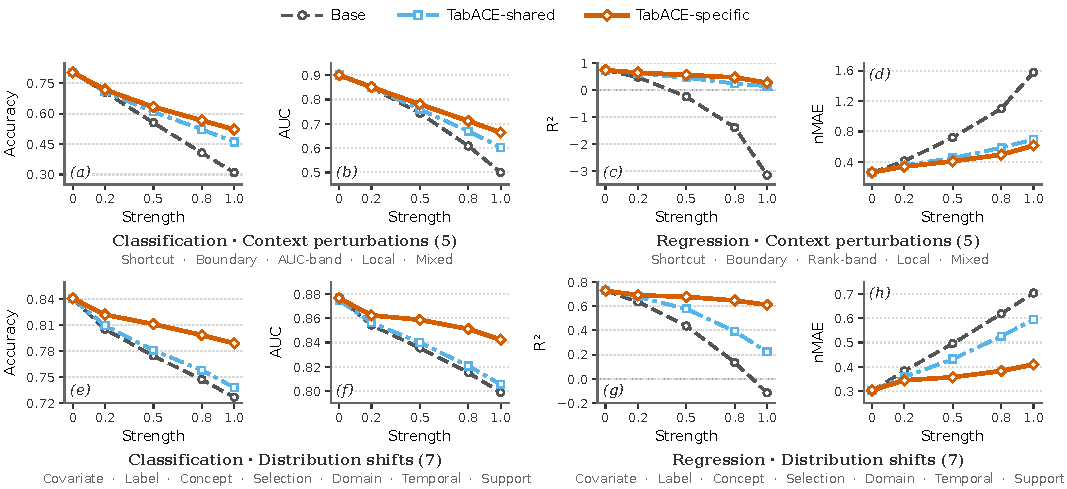
\includegraphics[width=\textwidth]{figures/tabace_strength_comparison.pdf}
  \caption{OpenML 基准上不同问题强度下的性能。分类面板使用 OpenML-CC18，回归面板使用 OpenML-CTR23。第一行对五种受控上下文扰动进行宏平均，第二行对七种分布偏移进行宏平均。}
  \label{fig:semisynthetic-strength}
\end{figure}

\clearpage
% 中文版保留原始数值与方法名称。
\definecolor{tabaceSharedRow}{HTML}{EAF4FB}
\definecolor{tabaceSpecificRow}{HTML}{FFF4D6}
\definecolor{tabaceSharedText}{HTML}{0072B2}
\definecolor{tabaceSpecificText}{HTML}{D55E00}
\ifdefined\ICLRLayout
\begin{table}[H]
\else
\begin{table}[H]
\fi
  \caption{OpenML-CC18 分类与 OpenML-CTR23 回归任务上的整体性能。扰动和偏移区块分别在五种和七种变化类别的全部非零强度上进行宏平均。}
  \label{tab:overall-performance}
  \centering
  \scriptsize
  \setlength{\tabcolsep}{2.0pt}
  \renewcommand{\arraystretch}{0.98}
  \begin{tabular}{@{}l*{12}{c}@{}}
    \toprule
    & \multicolumn{4}{c}{干净数据}
    & \multicolumn{4}{c}{五种扰动（平均）}
    & \multicolumn{4}{c}{七种偏移（平均）} \\
    \cmidrule(lr){2-5}\cmidrule(lr){6-9}\cmidrule(lr){10-13}
    & \multicolumn{2}{c}{分类} & \multicolumn{2}{c}{回归}
    & \multicolumn{2}{c}{分类} & \multicolumn{2}{c}{回归}
    & \multicolumn{2}{c}{分类} & \multicolumn{2}{c}{回归} \\
    \cmidrule(lr){2-3}\cmidrule(lr){4-5}
    \cmidrule(lr){6-7}\cmidrule(lr){8-9}
    \cmidrule(lr){10-11}\cmidrule(lr){12-13}
    方法
    & Acc$\uparrow$ & AUC$\uparrow$ & $R^2\uparrow$ & nRMSE$\downarrow$
    & Acc$\uparrow$ & AUC$\uparrow$ & $R^2\uparrow$ & nRMSE$\downarrow$
    & Acc$\uparrow$ & AUC$\uparrow$ & $R^2\uparrow$ & nRMSE$\downarrow$ \\
    \midrule
    \multicolumn{13}{@{}l}{\textit{非 TFM 基线}} \\
    LogReg/Ridge + HPO & 0.754 & 0.867 & 0.543 & 0.684 & 0.418 & 0.582 & -0.559 & 1.175 & 0.719 & 0.775 & -0.490 & 0.851 \\
    SVM/SVR + HPO & 0.777 & 0.879 & 0.492 & 0.703 & 0.449 & 0.611 & -0.872 & 1.255 & 0.757 & 0.793 & 0.010 & 0.873 \\
    kNN + HPO & 0.726 & 0.856 & 0.587 & 0.656 & 0.489 & 0.647 & -1.245 & 1.396 & 0.743 & 0.775 & 0.327 & 0.779 \\
    RF + HPO & 0.776 & 0.886 & 0.676 & 0.561 & 0.451 & 0.649 & -1.218 & 1.335 & 0.760 & 0.810 & 0.385 & 0.724 \\
    LightGBM + HPO & 0.776 & 0.884 & 0.697 & 0.529 & 0.463 & 0.639 & -1.215 & 1.337 & 0.759 & 0.796 & 0.350 & 0.736 \\
    CatBoost + HPO & 0.782 & 0.890 & 0.708 & 0.514 & 0.479 & 0.653 & -1.372 & 1.368 & 0.770 & 0.811 & 0.381 & 0.711 \\
    XGBoost + HPO & 0.774 & 0.885 & 0.702 & 0.525 & 0.455 & 0.640 & -1.323 & 1.359 & 0.751 & 0.796 & 0.278 & 0.767 \\
    MLP + HPO & 0.729 & 0.858 & 0.583 & 0.568 & 0.435 & 0.604 & -1.007 & 1.272 & 0.741 & 0.767 & 0.066 & 0.828 \\
    FT-Transformer & 0.745 & 0.861 & 0.657 & 0.568 & 0.456 & 0.619 & -1.256 & 1.353 & 0.716 & 0.765 & 0.210 & 0.822 \\
    TabM & 0.735 & 0.866 & 0.655 & 0.577 & 0.454 & 0.614 & -1.100 & 1.324 & 0.699 & 0.743 & 0.212 & 0.811 \\
    TabulaRNN & 0.722 & 0.856 & 0.580 & 0.648 & 0.454 & 0.625 & -0.851 & 1.270 & 0.718 & 0.754 & 0.205 & 0.845 \\
    MambaTab & 0.748 & 0.869 & 0.663 & 0.564 & 0.434 & 0.602 & -0.824 & 1.230 & 0.751 & 0.784 & 0.279 & 0.761 \\
    RealMLP & 0.762 & 0.872 & 0.694 & 0.527 & 0.448 & 0.614 & -1.258 & 1.326 & 0.758 & 0.793 & 0.240 & 0.749 \\
    \midrule
    LimiX-2M & 0.796 & 0.896 & 0.724 & 0.494 & 0.475 & 0.657 & -1.141 & 1.277 & 0.781 & 0.831 & 0.385 & 0.689 \\
    \rowcolor{tabaceSharedRow}
    \textcolor{tabaceSharedText}{\textbf{+ \method{}-shared}} & \textcolor{tabaceSharedText}{\textbf{0.796}} & \textcolor{tabaceSharedText}{\textbf{0.896}} & \textcolor{tabaceSharedText}{\textbf{0.725}} & \textcolor{tabaceSharedText}{\textbf{0.493}} & \textcolor{tabaceSharedText}{\textbf{0.542}} & \textcolor{tabaceSharedText}{\textbf{0.716}} & \textcolor{tabaceSharedText}{\textbf{-0.173}} & \textcolor{tabaceSharedText}{\textbf{1.059}} & \textcolor{tabaceSharedText}{\textbf{0.784}} & \textcolor{tabaceSharedText}{\textbf{0.835}} & \textcolor{tabaceSharedText}{\textbf{0.498}} & \textcolor{tabaceSharedText}{\textbf{0.659}} \\
    \rowcolor{tabaceSpecificRow}
    \textcolor{tabaceSpecificText}{\textbf{+ \method{}-specific}} & \textcolor{tabaceSpecificText}{\textbf{0.796}} & \textcolor{tabaceSpecificText}{\textbf{0.896}} & \textcolor{tabaceSpecificText}{\textbf{0.725}} & \textcolor{tabaceSpecificText}{\textbf{0.493}} & \textcolor{tabaceSpecificText}{\textbf{0.628}} & \textcolor{tabaceSpecificText}{\textbf{0.769}} & \textcolor{tabaceSpecificText}{\textbf{0.053}} & \textcolor{tabaceSpecificText}{\textbf{0.947}} & \textcolor{tabaceSpecificText}{\textbf{0.804}} & \textcolor{tabaceSpecificText}{\textbf{0.847}} & \textcolor{tabaceSpecificText}{\textbf{0.629}} & \textcolor{tabaceSpecificText}{\textbf{0.563}} \\
    \midrule
    TabICL-v2 & 0.804 & 0.901 & 0.739 & 0.476 & 0.494 & 0.676 & -1.077 & 1.270 & 0.763 & 0.826 & 0.273 & 0.730 \\
    \rowcolor{tabaceSharedRow}
    \textcolor{tabaceSharedText}{\textbf{+ \method{}-shared}} & \textcolor{tabaceSharedText}{\textbf{0.804}} & \textcolor{tabaceSharedText}{\textbf{0.901}} & \textcolor{tabaceSharedText}{\textbf{0.738}} & \textcolor{tabaceSharedText}{\textbf{0.478}} & \textcolor{tabaceSharedText}{\textbf{0.575}} & \textcolor{tabaceSharedText}{\textbf{0.720}} & \textcolor{tabaceSharedText}{\textbf{0.363}} & \textcolor{tabaceSharedText}{\textbf{0.783}} & \textcolor{tabaceSharedText}{\textbf{0.772}} & \textcolor{tabaceSharedText}{\textbf{0.831}} & \textcolor{tabaceSharedText}{\textbf{0.467}} & \textcolor{tabaceSharedText}{\textbf{0.659}} \\
    \rowcolor{tabaceSpecificRow}
    \textcolor{tabaceSpecificText}{\textbf{+ \method{}-specific}} & \textcolor{tabaceSpecificText}{\textbf{0.804}} & \textcolor{tabaceSpecificText}{\textbf{0.900}} & \textcolor{tabaceSpecificText}{\textbf{0.738}} & \textcolor{tabaceSpecificText}{\textbf{0.476}} & \textcolor{tabaceSpecificText}{\textbf{0.610}} & \textcolor{tabaceSpecificText}{\textbf{0.752}} & \textcolor{tabaceSpecificText}{\textbf{0.485}} & \textcolor{tabaceSpecificText}{\textbf{0.708}} & \textcolor{tabaceSpecificText}{\textbf{0.805}} & \textcolor{tabaceSpecificText}{\textbf{0.854}} & \textcolor{tabaceSpecificText}{\textbf{0.655}} & \textcolor{tabaceSpecificText}{\textbf{0.535}} \\
    \midrule
    TabPFN-v3 & 0.793 & 0.893 & 0.739 & 0.476 & 0.457 & 0.636 & -1.253 & 1.313 & 0.758 & 0.809 & 0.426 & 0.669 \\
    \rowcolor{tabaceSharedRow}
    \textcolor{tabaceSharedText}{\textbf{+ \method{}-shared}} & \textcolor{tabaceSharedText}{\textbf{0.792}} & \textcolor{tabaceSharedText}{\textbf{0.893}} & \textcolor{tabaceSharedText}{\textbf{0.739}} & \textcolor{tabaceSharedText}{\textbf{0.480}} & \textcolor{tabaceSharedText}{\textbf{0.553}} & \textcolor{tabaceSharedText}{\textbf{0.697}} & \textcolor{tabaceSharedText}{\textbf{0.237}} & \textcolor{tabaceSharedText}{\textbf{0.834}} & \textcolor{tabaceSharedText}{\textbf{0.770}} & \textcolor{tabaceSharedText}{\textbf{0.817}} & \textcolor{tabaceSharedText}{\textbf{0.460}} & \textcolor{tabaceSharedText}{\textbf{0.656}} \\
    \rowcolor{tabaceSpecificRow}
    \textcolor{tabaceSpecificText}{\textbf{+ \method{}-specific}} & \textcolor{tabaceSpecificText}{\textbf{0.792}} & \textcolor{tabaceSpecificText}{\textbf{0.893}} & \textcolor{tabaceSpecificText}{\textbf{0.739}} & \textcolor{tabaceSpecificText}{\textbf{0.477}} & \textcolor{tabaceSpecificText}{\textbf{0.593}} & \textcolor{tabaceSpecificText}{\textbf{0.739}} & \textcolor{tabaceSpecificText}{\textbf{0.588}} & \textcolor{tabaceSpecificText}{\textbf{0.635}} & \textcolor{tabaceSpecificText}{\textbf{0.788}} & \textcolor{tabaceSpecificText}{\textbf{0.835}} & \textcolor{tabaceSpecificText}{\textbf{0.620}} & \textcolor{tabaceSpecificText}{\textbf{0.565}} \\
    \midrule
    TabDPT v1.2 & 0.779 & 0.891 & 0.731 & 0.488 & 0.448 & 0.631 & -1.152 & 1.300 & 0.774 & 0.821 & 0.514 & 0.633 \\
    \rowcolor{tabaceSharedRow}
    \textcolor{tabaceSharedText}{\textbf{+ \method{}-shared}} & \textcolor{tabaceSharedText}{\textbf{0.779}} & \textcolor{tabaceSharedText}{\textbf{0.891}} & \textcolor{tabaceSharedText}{\textbf{0.730}} & \textcolor{tabaceSharedText}{\textbf{0.491}} & \textcolor{tabaceSharedText}{\textbf{0.548}} & \textcolor{tabaceSharedText}{\textbf{0.694}} & \textcolor{tabaceSharedText}{\textbf{0.329}} & \textcolor{tabaceSharedText}{\textbf{0.803}} & \textcolor{tabaceSharedText}{\textbf{0.781}} & \textcolor{tabaceSharedText}{\textbf{0.831}} & \textcolor{tabaceSharedText}{\textbf{0.547}} & \textcolor{tabaceSharedText}{\textbf{0.614}} \\
    \rowcolor{tabaceSpecificRow}
    \textcolor{tabaceSpecificText}{\textbf{+ \method{}-specific}} & \textcolor{tabaceSpecificText}{\textbf{0.779}} & \textcolor{tabaceSpecificText}{\textbf{0.891}} & \textcolor{tabaceSpecificText}{\textbf{0.730}} & \textcolor{tabaceSpecificText}{\textbf{0.488}} & \textcolor{tabaceSpecificText}{\textbf{0.600}} & \textcolor{tabaceSpecificText}{\textbf{0.746}} & \textcolor{tabaceSpecificText}{\textbf{0.443}} & \textcolor{tabaceSpecificText}{\textbf{0.733}} & \textcolor{tabaceSpecificText}{\textbf{0.805}} & \textcolor{tabaceSpecificText}{\textbf{0.846}} & \textcolor{tabaceSpecificText}{\textbf{0.610}} & \textcolor{tabaceSpecificText}{\textbf{0.572}} \\
    \bottomrule
  \end{tabular}
\ifdefined\ICLRLayout
\end{table}
\else
\end{table}
\fi

\fi

\section{实验}
\label{sec:experiments}

\subsection{实验设置}
\label{sec:experimental_setup}

\paragraph{评估轨道。}
我们在公开 OpenML 基准和全合成数据上评估 TabACE。OpenML 轨道的分类任务来自 OpenML-CC18~\citep{bischl2021openml}，回归任务来自 OpenML-CTR23~\citep{fischer2023openmlctr23}。受控变化采用五折数据集级折外（OOF）评估：策略在其余四折上拟合，并在留出数据集上保持固定。强度为零时，上下文与输入均不改变。合成轨道使用受控数据生成过程，分别考察问题类别与强度的影响。

\paragraph{问题与配置。}
两个轨道均覆盖五种源上下文扰动（Shortcut、Boundary、AUC/Rank-band、Local 和 Mixed）与七种分布偏移（Covariate、Label、Concept、Selection、Domain、Temporal 和 Support），强度取 $0$、$0.2$、$0.5$、$0.8$ 和 $1.0$。Base 表示不进行上下文集成的冻结主干模型。Shared 在所有预定义变化上采用固定上下文库；Specific 则根据目标推理前给定的变化类别选择并融合候选上下文。除非另行注明预测器，所有次要实验均采用冻结的 TabICL-v2，Base 表示其未经修改的预测。附录列出全部算子与上下文布局。

% Register this float before the final setup paragraphs so that the arXiv
% layout places it at the top of page 7.  The ICLR layout inserts the same
% figure at the corresponding results subsection instead.
\ifdefined\ICLRLayout\else
\clearpage
\begin{figure}[H]
  \centering
  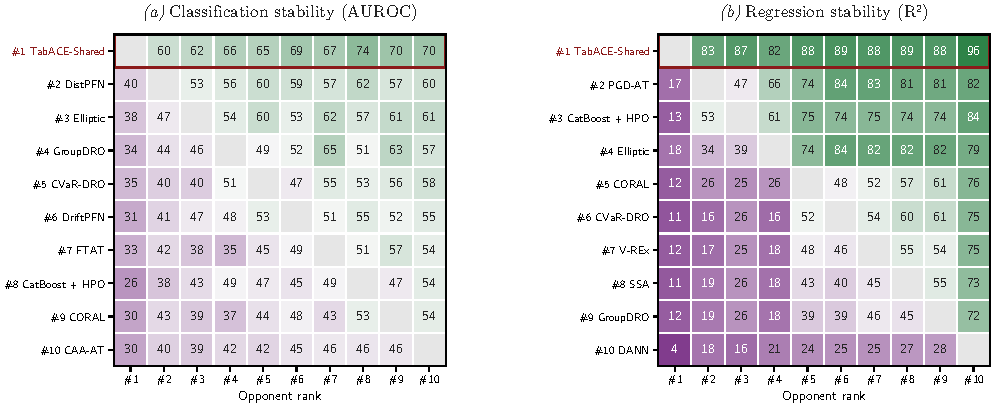
\includegraphics[width=0.88\textwidth]{figures/tabace_synthetic_stability.pdf}
  \caption{在 180 个对齐的“随机种子--DGP--场景”实验单元上的成对稳定性。分类使用经机会水平校正的 AUROC 边际退化，回归使用归一化 $R^2$ 退化。单元格表示行方法取得较小性能下降的频率；差异不超过 $0.001$ 时记为平局。}
  \label{fig:synthetic-stability}
\end{figure}

\begin{figure}[H]
  \centering
  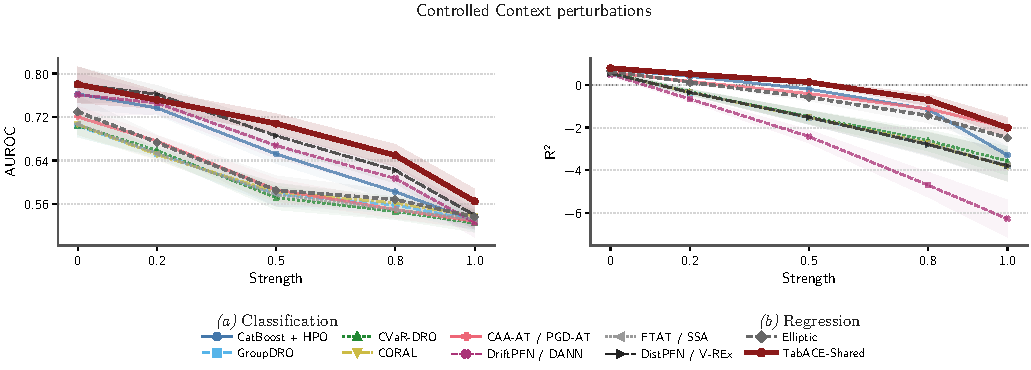
\includegraphics[width=0.94\textwidth]{figures/tabace_controlled_response.pdf}
  \caption{全合成设置下对受控上下文扰动的响应。各面板分别报告分类 AUROC 与回归 $R^2$；曲线汇总五种扰动类别上的对齐实验单元，阴影带表示 $95\%$ bootstrap 区间。}
  \label{fig:synthetic-controlled-response}
\end{figure}
\fi

\paragraph{任务与指标。}
分类任务报告 Accuracy 和 AUROC，回归任务报告 $R^2$、nMAE 与 nRMSE。稳健性排名和强度响应图分别使用 AUROC 与 $R^2$。

\paragraph{基线。}
OpenML 实验比较经过调优的常规预测器、树模型、神经网络模型和冻结的基础模型，其中包括 LimiX-2M 检查点（下文简称 LimiX）~\citep{wang2026limix2m}。合成实验比较稳健学习、对抗训练与分布适配基线。附录列出所有方法及其适用任务，并说明使用 LimiX 覆盖完整 OpenML 测试套件的兼容性方案。

\ifdefined\ICLRLayout
\clearpage
\begin{figure}[H]
  \centering
  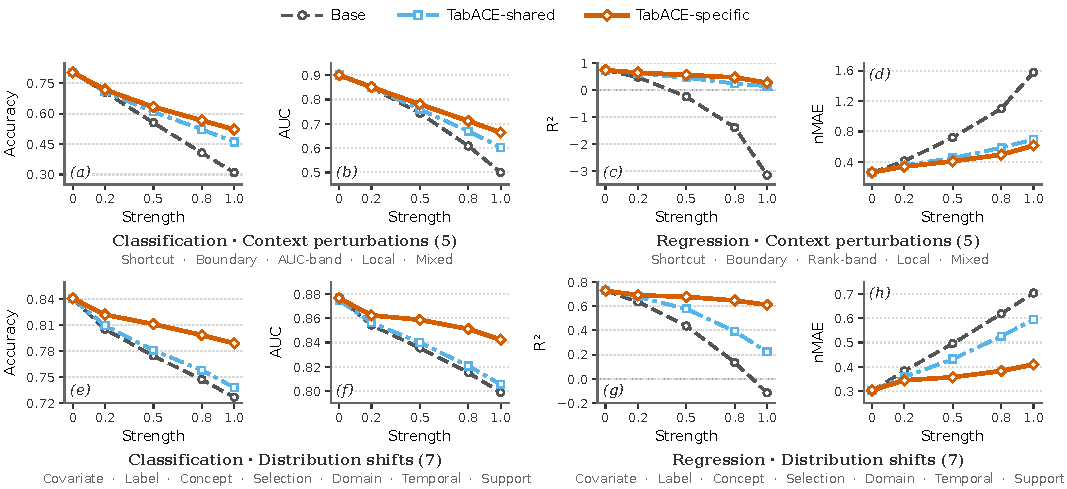
\includegraphics[width=\textwidth]{figures/tabace_strength_comparison.pdf}
  \caption{OpenML 基准上不同问题强度下的性能。分类面板使用 OpenML-CC18，回归面板使用 OpenML-CTR23。第一行对五种受控上下文扰动进行宏平均，第二行对七种分布偏移进行宏平均。}
  \label{fig:semisynthetic-strength}
\end{figure}
\fi

\paragraph{选择方案。}
在每个外层折内，上下文配置、分支权重与整合参数均在其余四个数据集折生成的校准 episode 上拟合，并在留出数据集评估前固定。这些 episode 覆盖已注册的条件，但拟合策略和留出推理均不接收变化强度。所有方法使用相同的外层折与评估样本，留出目标标签仅用于计算最终指标。

% Keep the two compact tables and the inference-cost figure together at the
% top of arXiv page 8, after the page-7 figures and setup text.
\ifdefined\ICLRLayout\else
\clearpage
\definecolor{sharedblue}{RGB}{31,84,147}
\definecolor{specificred}{RGB}{213,94,0}

\begin{table}[H]
  \centering
  \begin{minipage}[t]{0.61\textwidth}
    \vspace{0pt}
    \centering
    \caption{自然地理偏移与时间偏移下的 ID 和 OOD Accuracy。}
    \label{tab:natural-shifts}
    \small
    \setlength{\tabcolsep}{4.0pt}
    \renewcommand{\arraystretch}{1.02}
    \begin{tabular}{@{}llccc@{}}
      \toprule
      方法 & 域 & Employment & Income & TravelTime \\
      \midrule
      \multicolumn{5}{@{}l}{\textit{地理：California $\rightarrow$ Michigan（2018）}} \\
      Base & ID  & 0.7922 & 0.7888 & 0.5912 \\
           & OOD & 0.8043 & 0.7655 & 0.5472 \\
      Shared & ID
        & \textcolor{sharedblue}{0.7948} & \textcolor{sharedblue}{0.7951}
        & \textcolor{sharedblue}{0.5945} \\
           & OOD
        & \textcolor{sharedblue}{0.8078} & \textcolor{sharedblue}{0.7832}
        & \textcolor{sharedblue}{0.5961} \\
      Specific & ID
        & \textcolor{specificred}{\textbf{0.7979}}
        & \textcolor{specificred}{\textbf{0.7955}}
        & \textcolor{specificred}{\textbf{0.6002}} \\
           & OOD
        & \textcolor{specificred}{\textbf{0.8089}}
        & \textcolor{specificred}{\textbf{0.7840}}
        & \textcolor{specificred}{\textbf{0.6034}} \\
      \addlinespace[2pt]
      \multicolumn{5}{@{}l}{\textit{时间：California 2014 $\rightarrow$ 2018}} \\
      Base & ID  & 0.7704 & 0.7926 & 0.5951 \\
           & OOD & 0.7847 & 0.7844 & 0.5908 \\
      Shared & ID
        & \textcolor{sharedblue}{0.7751} & \textcolor{sharedblue}{0.7968}
        & \textcolor{sharedblue}{0.6032} \\
           & OOD
        & \textcolor{sharedblue}{0.7900} & \textcolor{sharedblue}{0.7937}
        & \textcolor{sharedblue}{0.5975} \\
      Specific & ID
        & \textcolor{specificred}{\textbf{0.7757}}
        & \textcolor{specificred}{\textbf{0.7980}}
        & \textcolor{specificred}{\textbf{0.6061}} \\
           & OOD
        & \textcolor{specificred}{\textbf{0.7916}}
        & \textcolor{specificred}{\textbf{0.7947}}
        & \textcolor{specificred}{\textbf{0.5981}} \\
      \bottomrule
    \end{tabular}
  \end{minipage}\hfill
  \begin{minipage}[t]{0.36\textwidth}
    \vspace{0pt}
    \centering
    \caption{上下文集成相对于各未经修改的常规预测器的增益。}
    \label{tab:traditional-backbone-gains}
    \small
    \setlength{\tabcolsep}{4.0pt}
    \renewcommand{\arraystretch}{1.02}
    \begin{tabular}{@{}lcc@{}}
      \toprule
      \multicolumn{3}{c}{分类：$\Delta$Accuracy $\uparrow$} \\
      \cmidrule(lr){1-3}
      预测器 & Shared & Specific \\
      \midrule
      kNN & \textcolor{sharedblue}{+0.0167}
        & \textcolor{specificred}{\textbf{+0.0227}} \\
      Logistic & \textcolor{sharedblue}{+0.0069}
        & \textcolor{specificred}{\textbf{+0.0287}} \\
      CatBoost & \textcolor{sharedblue}{+0.0145}
        & \textcolor{specificred}{\textbf{+0.0287}} \\
      MLP & \textcolor{sharedblue}{+0.0107}
        & \textcolor{specificred}{\textbf{+0.0285}} \\
      \addlinespace[5pt]
      \multicolumn{3}{c}{回归：$\Delta R^2$ $\uparrow$} \\
      \cmidrule(lr){1-3}
      预测器 & Shared & Specific \\
      \midrule
      kNN & \textcolor{sharedblue}{+0.0203}
        & \textcolor{specificred}{\textbf{+0.0654}} \\
      Ridge & \textcolor{sharedblue}{+0.1425}
        & \textcolor{specificred}{\textbf{+0.1966}} \\
      CatBoost & \textcolor{sharedblue}{+0.1279}
        & \textcolor{specificred}{\textbf{+0.1740}} \\
      MLP & \textcolor{sharedblue}{+0.0499}
        & \textcolor{specificred}{\textbf{+0.1645}} \\
      \bottomrule
    \end{tabular}
  \end{minipage}
\end{table}


\begin{figure}[H]
  \centering
  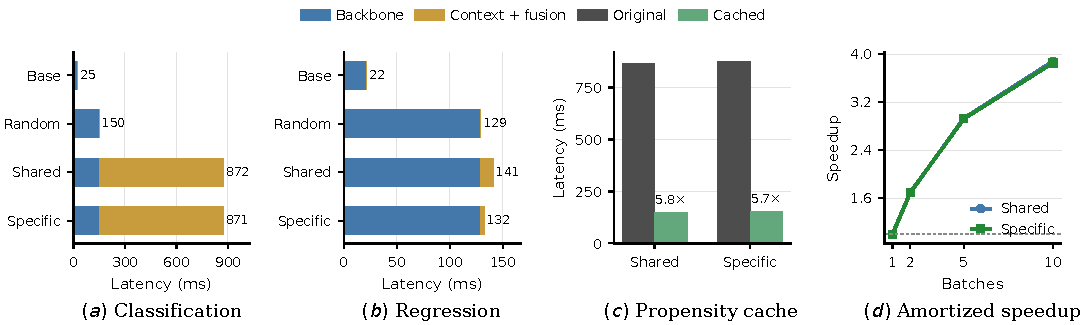
\includegraphics[width=0.96\textwidth]{figures/tabace_inference_cost_ablation.pdf}
  \caption{固定五上下文 Shared 库与单独评估的 Base 分支的推理成本消融。面板 (a--b) 分解中位延迟；(c) 比较原始推理与缓存推理；(d) 在摊销加速比中计入一次性缓存建立成本。}
  \label{fig:inference-cost}
\end{figure}
\fi

\subsection{OpenML 基准上的操控实验}
\label{sec:semi_synthetic_results}

上下文扰动轨道包含 72 个 OpenML-CC18 分类数据集和 35 个 OpenML-CTR23 回归数据集；分布偏移轨道分别包含 35 个和 33 个数据集。干净数据性能使用原始上下文与输入计算。

% Original sources for every named Table 1 and Table 4 predictor. The
% non-printing citations preserve the compact result layout while ensuring
% that each baseline has a corresponding bibliography entry.
\nocite{cox1958binary,hoerl1970ridge,cortes1995svm,drucker1996svr,
cover1967knn,breiman2001randomforests,ke2017lightgbm,
prokhorenkova2018catboost,chen2016xgboost,rumelhart1986backprop,
gorishniy2021fttransformer,gorishniy2025tabm,thielmann2024tabularnn,
ahamed2024mambatab,holzmueller2024realmlp,qu2026tabiclv2,
grinsztajn2026tabpfn3technicalreport,wang2026limix2m,ma2025tabdpt}

表~\ref{tab:overall-performance} 比较了 13 个常规或神经网络基线与四个冻结的表格基础模型：LimiX-2M、TabICL-v2、TabPFN-v3 和 TabDPT v1.2。相对于 Base，Shared 改善了所有非零强度下的扰动与偏移指标；Specific 在每项比较中进一步提升性能。干净数据得分基本不变。基线配置、引用以及覆盖完整测试套件的 LimiX 兼容性方案见附录~\ref{app:baseline_details}。

\paragraph{OpenML 任务上的强度响应。}
图~\ref{fig:semisynthetic-strength} 报告全部五个强度，并对数据集以及五种扰动或七种偏移类别赋予相同权重。强度为零时，三种配置的性能接近。随着强度增加，Base 下降最快，Shared 持续减缓下降，Specific 则进一步改善；在每个非零强度下，Specific 在全部八个面板中均取得最高得分。

\subsection{全合成稳健性实验}
\label{sec:results}

\paragraph{实验方案与基线。}
我们在 12 个合成问题类别上评估固定五槽位的 Shared 接口。这些问题由五种具有相关特征与受控目标的数据生成过程产生。每个问题类别均在五个强度和三个随机种子下测试。比较对象包括附录~\ref{app:baseline_details} 所列的九种稳健学习、对抗训练与分布适配基线。对齐的评估单元在分类任务中使用 AUROC，在回归任务中使用 $R^2$。

\ifdefined\ICLRLayout
\begin{figure}[H]
  \centering
  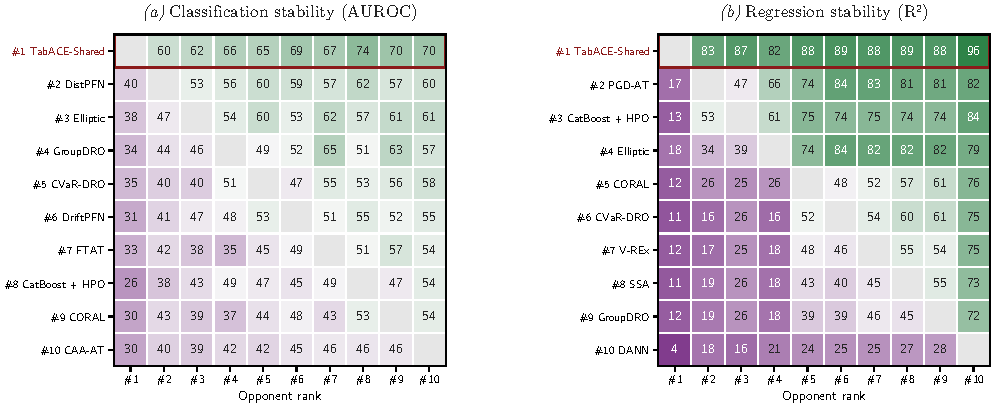
\includegraphics[width=0.88\textwidth]{figures/tabace_synthetic_stability.pdf}
  \caption{在 180 个对齐的“随机种子--DGP--场景”实验单元上的成对稳定性。分类使用经机会水平校正的 AUROC 边际退化，回归使用归一化 $R^2$ 退化。单元格表示行方法取得较小性能下降的频率；差异不超过 $0.001$ 时记为平局。}
  \label{fig:synthetic-stability}
\end{figure}

\begin{figure}[H]
  \centering
  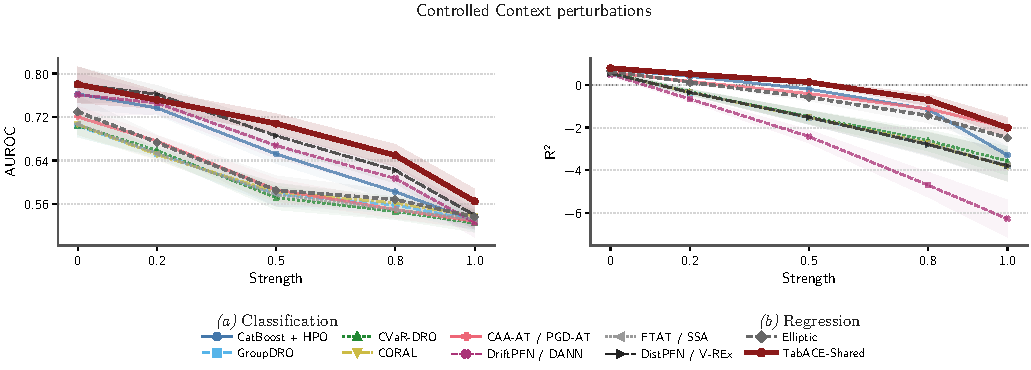
\includegraphics[width=0.94\textwidth]{figures/tabace_controlled_response.pdf}
  \caption{全合成设置下对受控上下文扰动的响应。各面板分别报告分类 AUROC 与回归 $R^2$；曲线汇总五种扰动类别上的对齐实验单元，阴影带表示 $95\%$ bootstrap 区间。}
  \label{fig:synthetic-controlled-response}
\end{figure}
\fi

\paragraph{稳定性。}
对于每个“随机种子--DGP--场景”实验单元，我们对四个非零强度取平均，并分别以干净数据 AUROC 的判别裕量和干净数据 $R^2$ 对分类与回归的性能退化进行归一化。具体定义见附录~\ref{app:metrics_reporting}。图~\ref{fig:synthetic-stability} 报告 180 个对齐实验单元上的成对胜率。TabACE-Shared 在分类和回归中均排名第一，平均胜率分别为 $67.0\%$ 和 $87.6\%$。

\ifdefined\ICLRLayout
\paragraph{强度响应。}
图~\ref{fig:synthetic-controlled-response} 报告受控上下文扰动下的分类 AUROC 与回归 $R^2$。曲线对对齐的 DGP、问题与随机种子单元赋予相同权重，并给出 $95\%$ bootstrap 区间。从强度 $0.5$ 起，TabACE-Shared 取得最高的分类 AUROC。上下文数量与聚合规则的消融实验见附录。

\subsection{补充实验}
\label{sec:additional-experiments}

\paragraph{自然分布偏移。}
Folktables~\citep{ding2021folktables} 提供了 2018 年从加利福尼亚州到密歇根州的地理偏移，以及加利福尼亚州内从 2014 年到 2018 年的时间偏移。表~\ref{tab:natural-shifts} 报告 Employment、Income 和 TravelTime 任务上的 ID 与 OOD Accuracy。Specific 在所有设置下均取得最高得分。

\definecolor{sharedblue}{RGB}{31,84,147}
\definecolor{specificred}{RGB}{213,94,0}

\begin{table}[H]
  \centering
  \begin{minipage}[t]{0.61\textwidth}
    \vspace{0pt}
    \centering
    \caption{自然地理偏移与时间偏移下的 ID 和 OOD Accuracy。}
    \label{tab:natural-shifts}
    \small
    \setlength{\tabcolsep}{4.0pt}
    \renewcommand{\arraystretch}{1.02}
    \begin{tabular}{@{}llccc@{}}
      \toprule
      方法 & 域 & Employment & Income & TravelTime \\
      \midrule
      \multicolumn{5}{@{}l}{\textit{地理：California $\rightarrow$ Michigan（2018）}} \\
      Base & ID  & 0.7922 & 0.7888 & 0.5912 \\
           & OOD & 0.8043 & 0.7655 & 0.5472 \\
      Shared & ID
        & \textcolor{sharedblue}{0.7948} & \textcolor{sharedblue}{0.7951}
        & \textcolor{sharedblue}{0.5945} \\
           & OOD
        & \textcolor{sharedblue}{0.8078} & \textcolor{sharedblue}{0.7832}
        & \textcolor{sharedblue}{0.5961} \\
      Specific & ID
        & \textcolor{specificred}{\textbf{0.7979}}
        & \textcolor{specificred}{\textbf{0.7955}}
        & \textcolor{specificred}{\textbf{0.6002}} \\
           & OOD
        & \textcolor{specificred}{\textbf{0.8089}}
        & \textcolor{specificred}{\textbf{0.7840}}
        & \textcolor{specificred}{\textbf{0.6034}} \\
      \addlinespace[2pt]
      \multicolumn{5}{@{}l}{\textit{时间：California 2014 $\rightarrow$ 2018}} \\
      Base & ID  & 0.7704 & 0.7926 & 0.5951 \\
           & OOD & 0.7847 & 0.7844 & 0.5908 \\
      Shared & ID
        & \textcolor{sharedblue}{0.7751} & \textcolor{sharedblue}{0.7968}
        & \textcolor{sharedblue}{0.6032} \\
           & OOD
        & \textcolor{sharedblue}{0.7900} & \textcolor{sharedblue}{0.7937}
        & \textcolor{sharedblue}{0.5975} \\
      Specific & ID
        & \textcolor{specificred}{\textbf{0.7757}}
        & \textcolor{specificred}{\textbf{0.7980}}
        & \textcolor{specificred}{\textbf{0.6061}} \\
           & OOD
        & \textcolor{specificred}{\textbf{0.7916}}
        & \textcolor{specificred}{\textbf{0.7947}}
        & \textcolor{specificred}{\textbf{0.5981}} \\
      \bottomrule
    \end{tabular}
  \end{minipage}\hfill
  \begin{minipage}[t]{0.36\textwidth}
    \vspace{0pt}
    \centering
    \caption{上下文集成相对于各未经修改的常规预测器的增益。}
    \label{tab:traditional-backbone-gains}
    \small
    \setlength{\tabcolsep}{4.0pt}
    \renewcommand{\arraystretch}{1.02}
    \begin{tabular}{@{}lcc@{}}
      \toprule
      \multicolumn{3}{c}{分类：$\Delta$Accuracy $\uparrow$} \\
      \cmidrule(lr){1-3}
      预测器 & Shared & Specific \\
      \midrule
      kNN & \textcolor{sharedblue}{+0.0167}
        & \textcolor{specificred}{\textbf{+0.0227}} \\
      Logistic & \textcolor{sharedblue}{+0.0069}
        & \textcolor{specificred}{\textbf{+0.0287}} \\
      CatBoost & \textcolor{sharedblue}{+0.0145}
        & \textcolor{specificred}{\textbf{+0.0287}} \\
      MLP & \textcolor{sharedblue}{+0.0107}
        & \textcolor{specificred}{\textbf{+0.0285}} \\
      \addlinespace[5pt]
      \multicolumn{3}{c}{回归：$\Delta R^2$ $\uparrow$} \\
      \cmidrule(lr){1-3}
      预测器 & Shared & Specific \\
      \midrule
      kNN & \textcolor{sharedblue}{+0.0203}
        & \textcolor{specificred}{\textbf{+0.0654}} \\
      Ridge & \textcolor{sharedblue}{+0.1425}
        & \textcolor{specificred}{\textbf{+0.1966}} \\
      CatBoost & \textcolor{sharedblue}{+0.1279}
        & \textcolor{specificred}{\textbf{+0.1740}} \\
      MLP & \textcolor{sharedblue}{+0.0499}
        & \textcolor{specificred}{\textbf{+0.1645}} \\
      \bottomrule
    \end{tabular}
  \end{minipage}
\end{table}


\begin{figure}[H]
  \centering
  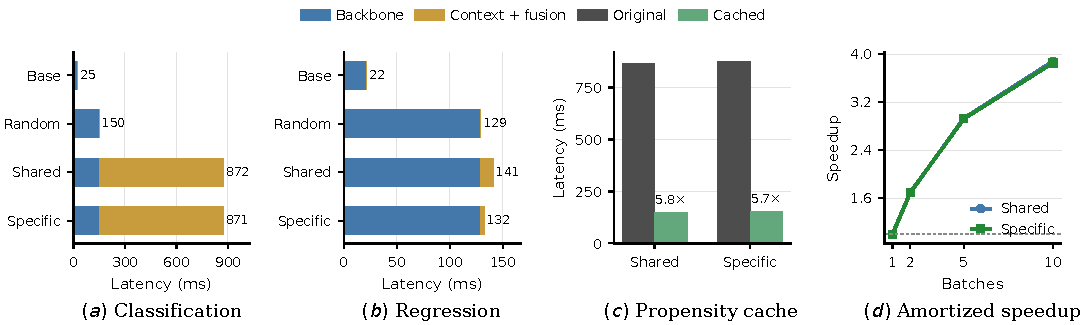
\includegraphics[width=0.96\textwidth]{figures/tabace_inference_cost_ablation.pdf}
  \caption{五个替代上下文和单独评估的 Base 分支的推理成本消融。面板 (a--b) 分解中位延迟；(c) 比较原始推理与缓存推理；(d) 在摊销加速比中计入一次性缓存建立成本。}
  \label{fig:inference-cost}
\end{figure}
\else
\paragraph{强度响应。}
图~\ref{fig:synthetic-controlled-response} 报告受控上下文扰动下的分类 AUROC 与回归 $R^2$。曲线对对齐的 DGP、问题与随机种子单元赋予相同权重，并给出 $95\%$ bootstrap 区间。从强度 $0.5$ 起，TabACE-Shared 取得最高的分类 AUROC。上下文数量与聚合规则的消融实验见附录。
\fi

\ifdefined\ICLRLayout\else
\subsection{补充实验}
\label{sec:additional-experiments}

\paragraph{自然分布偏移。}
Folktables~\citep{ding2021folktables} 提供了 2018 年从加利福尼亚州到密歇根州的地理偏移，以及加利福尼亚州内从 2014 年到 2018 年的时间偏移。表~\ref{tab:natural-shifts} 报告 Employment、Income 和 TravelTime 任务上的 ID 与 OOD Accuracy。Specific 在所有设置下均取得最高得分。
\fi

\paragraph{常规预测器兼容性。}
将同一上下文集成接口应用于 kNN、Logistic/Ridge、CatBoost 和 MLP 后，Shared 在所有预测器上均提高了分类 Accuracy 和回归 $R^2$；Specific 则在全部八项比较中进一步提升性能（表~\ref{tab:traditional-backbone-gains}）。

\paragraph{推理成本。}
对于固定五上下文 Shared 库，图~\ref{fig:inference-cost} 将实际运行延迟分解为六次主干模型前向过程（Base 加五个替代上下文）以及上下文构造/融合。缓存可复用的倾向量使重复推理速度提高约 $5.7\times$。计入一次性缓存构造成本后，在十个批次上的摊销加速比仍约为 $3.9\times$。

\FloatBarrier

\section{结论}
\label{sec:conclusion}

\method{} 为固定预测器提供了一个推理时上下文集成接口。共识加权聚合彼此支持的预测，任务特定门控则使更新幅度与查询级证据相匹配。受控扰动、分布偏移、合成机制、自然偏移以及常规预测器上的实验表明，该接口能够在无需重新训练主干模型的情况下提高预测稳定性。

\paragraph{局限性与未来工作。}
Shared 不需要变化类别标识，而先验知情的 Specific 则研究另一种互补设置，即在推理前已知变化类别。当前实验覆盖了受控变化与若干自然偏移；更广泛的自然场景与高风险应用仍有待评估。评估多个上下文会增加推理成本，因此未来可研究根据无标签目标数据选择上下文，并进一步减少重复计算。

\section*{可复现性声明}

可复现性信息分布于正文与附录中。附录~\ref{app:theory} 给出完整理论分析；附录~\ref{app:experimental_setup} 说明数据集、划分、扰动、分布偏移、上下文构造、聚合方式与实现设置；附录~\ref{app:backbone-strength-curves} 和~\ref{app:supplemental_ablations} 分别报告按强度展开的完整结果与消融实验。所有实验结果均遵循附录~\ref{app:experimental_setup} 中的固定方案。受许可证限制的模型权重均来自其公开发布版本，本文不对其进行再分发。

\section*{人工智能工具使用声明}

作者使用生成式人工智能工具辅助润色写作、起草部分稿件，并支持投稿表格中未单独列出的任务。所有由人工智能辅助生成的内容均经作者审查与核验，作者对最终稿件承担责任。


\FloatBarrier
\bibliography{references}
\bibliographystyle{iclr2027_conference}

\appendix
\raggedbottom

\section*{附录内容}
\begingroup
\footnotesize
\hypersetup{linkcolor=black}
\setlength{\parindent}{0pt}
\newcommand{\apptocsection}[3]{%
  \vspace{0.22em}\noindent
  \textbf{\hyperref[#3]{#1\quad #2}}\nobreak\dotfill
  \textbf{\pageref*{#3}}\par}
\newcommand{\apptocsubsection}[3]{%
  \noindent\hspace{1.5em}\hyperref[#3]{#1\quad #2}\nobreak\dotfill
  \pageref*{#3}\par}
\apptocsection{A}{理论分析}{app:theory}
\apptocsubsection{A.1}{定理 1 的证明}{app:theorem-proof}
\apptocsubsection{A.2}{理论鲁棒性}{app:theoretical-robustness}
\apptocsection{B}{实验设置与可复现性}{app:experimental_setup}
\apptocsubsection{B.1}{评估协议}{app:evaluation_protocol}
\apptocsubsection{B.2}{受控扰动与分布偏移}{app:data_transformations}
\apptocsubsection{B.3}{比较方法与任务适用性}{app:baseline_details}
\apptocsubsection{B.4}{上下文构造}{app:context_construction}
\apptocsubsection{B.5}{实现细节}{app:implementation_details}
\apptocsection{C}{各主干模型的强度结果}{app:backbone-strength-curves}
\apptocsubsection{C.1}{TabICL-v2}{app:tabicl-strength-results}
\apptocsubsection{C.2}{其他主干模型}{app:additional-backbone-strength-results}
\apptocsection{D}{消融研究}{app:supplemental_ablations}
\apptocsubsection{D.1}{上下文预算}{app:context-budget}
\apptocsubsection{D.2}{聚合规则}{app:aggregation-rule}
\apptocsubsection{D.3}{固定上下文库组件消融}{app:fixed-bank-formula-diagnostic}
\apptocsubsection{D.4}{不同证据分箱下的门控行为}{app:gate-bin-analysis}
\endgroup
\hypersetup{linkcolor=linkblue}
\vspace{0.35em}

\section{理论分析}
\label{app:theory}

\subsection{定理的证明~\ref{thm:effective_context_repair}}
\label{app:theorem-proof}

\paragraph{分析设置与符号。}
\label{app:analysis-setup}

让 $\Phi=\{\phi_0,\ldots,\phi_R\}$ 成为从第~\ref{sec:context_interface} 设置的配置，其替代分支由 $\mathcal I(\Phi)=\{1,\ldots,R\}$ 索引。对于查询 $i$,文本 $r$ 产生 $o_i^{(r)}$,收到源端校准先验 $\pi_r$,并具有上下文库依赖的无标签分数 $\rho_i^{(r)}(\Phi)$,下面简称 $\rho_i^{(r)}$.
方程~\eqref{eq:task_aware_aggregation}形式权重$w_i^{(r)}$和总数$\bar o_i$最终预测是任务门控的混合物\[
o_i^{\mathrm{final}}=(1-\alpha_i)o_i^{(0)}+\alpha_i\bar o_i,
\qquad
\alpha_i=\alpha_{\max}U_iE_i,
\]在哪里$U_i,E_i,\alpha_{\max}\in[0,1]$.

对于一个损失曲的预测论点，上下文智能和总体改善是\[
\Delta_i^{(r)}
=\ell(o_i^{(0)},y_i^t)-\ell(o_i^{(r)},y_i^t),
\qquad
\Delta_i
=\ell(o_i^{(0)},y_i^t)-\ell(\bar o_i,y_i^t).
\]目标标签只出现在这些分析量中。构建，权重和基因集成在目标推断时仍然没有标签.$P_t^{(h)}$对于与变化类别相关的目标分布$h$其他$P_t$对于风险分析中使用的目标分布.

\paragraph{上下文互补性与有益覆盖。}
\label{app:repair-coverage}

固定式$\delta_+>0$定义
\begin{equation}
\mathcal H_r^h
=\{i:\Delta_i^{(r)}\geq\delta_+\},
\qquad
C_h(\Phi)
  =\Pr_{P_t^{(h)}}\!\left(i\in\bigcup_{r\in\mathcal I(\Phi)}\mathcal H_r^h\right).
\label{eq:potential_repair_coverage}
\end{equation}
集中的$\mathcal H_r^h$收集了相关问题$r$在家庭下可以改善$h$欧盟的措施至少有一个有利的背景.

添加一个配置$\phi_{r'}$通过
\begin{equation}
  C_h(\Phi\cup\{\phi_{r'}\})-C_h(\Phi)
  =\Pr_{P_t^{(h)}}\!\left(
    i\in\mathcal H_{r'}^h\setminus
    \bigcup_{r\in\mathcal I(\Phi)}\mathcal H_r^h
  \right).
  \label{eq:coverage_gain}
\end{equation}

\begin{lemma}[单调和子模块的环境覆盖]
\label{prop:coverage_submodular}覆盖功能$C_h$单调和子模块化.$\Phi_1\subseteq\Phi_2$其他$\phi_{r'}\notin\Phi_2$,
\begin{equation}
\begin{aligned}
0
&\leq C_h(\Phi_2\cup\{\phi_{r'}\})-C_h(\Phi_2)\\
&\leq C_h(\Phi_1\cup\{\phi_{r'}\})-C_h(\Phi_1).
\end{aligned}
\label{eq:coverage_diminishing_returns}
\end{equation}
\end{lemma}

\noindent\emph{证明.}让我们$\mathcal U_j=\bigcup_{r\in\mathcal I(\Phi_j)}\mathcal H_r^h$边缘覆盖率$r'$是\[
\Pr_{P_t^{(h)}}(i\in\mathcal H_{r'}^h\setminus\mathcal U_j).
\]自从$\mathcal U_1\subseteq\mathcal U_2$对于$\Phi_2$包含在此为$\Phi_1$两种不平等都会发生.
\hfill$\square$

方程~\eqref{eq:coverage_diminishing_returns}上下文库依赖的分数和关门控将覆盖与风险联系起来，通过$\mathcal G_i$在下面.

\paragraph{分数分离与有效权重。}
\label{app:evidence-separation}

固定上下文库 $\Phi$、查询 $i$ 和非空有效集合 $\mathcal G_i$。在式~\eqref{eq:repair_conditions} 的条件下，令
\[
N_{\mathcal G}
=\sum_{r\in\mathcal G_i}\pi_r e^{\rho_i^{(r)}},
\qquad
N_{\mathcal B}
=\sum_{r\in\mathcal I(\Phi)\setminus\mathcal G_i}\pi_r e^{\rho_i^{(r)}}.
\]
记 $\Pi_i=\sum_{r\in\mathcal G_i}\pi_r$，分数分离条件给出
\[
N_{\mathcal G}\geq\Pi_i e^{\rho_+},
\qquad
N_{\mathcal B}\leq(1-\Pi_i)e^{\rho_-}.
\]
因此，有效上下文上的归一化权重满足
\begin{equation}
W_i
=\frac{N_{\mathcal G}}{N_{\mathcal G}+N_{\mathcal B}}
\geq
\left[1+\frac{1-\Pi_i}{\Pi_i}
e^{-(\rho_+-\rho_-)}\right]^{-1}
=\underline W_i.
\label{eq:appendix_effective_weight}
\end{equation}
这一边界将两个路线暴露在更大的有效权重上:更大的前面质量$\Pi_i$并且更广泛的分数差距$\rho_+-\rho_-$曲率然后产生
\begin{equation}
\begin{aligned}
\Delta_i
&\geq\sum_{r=1}^{R} w_i^{(r)}\Delta_i^{(r)}\\
&\geq W_i\delta_+-(1-W_i)\delta_-\\
&\geq\underline W_i\delta_+-(1-\underline W_i)\delta_-
=\gamma_i.
\end{aligned}
\label{eq:appendix_aggregate_gain}
\end{equation}因此，当当一个人对一个人的$\underline W_i>\delta_-/(\delta_++\delta_-)$.

分数结合了源校准与目标侧的信任，协议或近距离。它们的联合排序决定了分离条件是否有效;下面的分析还涵盖了不完美的排序.

\paragraph{定理~\ref{thm:effective_context_repair} 的证明。}

式~\eqref{eq:appendix_effective_weight} 给出了 $W_i$ 的下界，式~\eqref{eq:appendix_aggregate_gain} 则证明 $\Delta_i\geq\gamma_i$。条件 $\underline W_i>\delta_-/(\delta_++\delta_-)$ 等价于 $\gamma_i>0$。

应用曲率到任务关键更新给出 \[
\begin{aligned}
\ell(o_i^{\mathrm{final}},y_i^t)
&\leq(1-\alpha_i)\ell(o_i^{(0)},y_i^t)
+\alpha_i\ell(\bar o_i,y_i^t),\\
\ell(o_i^{\mathrm{final}},y_i^t)-\ell(o_i^{(0)},y_i^t)
&\leq-\alpha_i\Delta_i.
\end{aligned}
\]对于$i\in\mathcal A_\Phi$总结结结为\[
\ell(o_i^{\mathrm{final}},y_i^t)-\ell(o_i^{(0)},y_i^t)
\leq-\alpha_{\max}U_iE_i\gamma_i.
\]
对于 $i\notin\mathcal A_\Phi$，曲率不等式给出
\[
\ell(o_i^{\mathrm{final}},y_i^t)-\ell(o_i^{(0)},y_i^t)
\leq\alpha_{\max}U_iE_i(-\Delta_i)_+.
\]接收了$P_t$预期和分开$\mathcal A_\Phi$并且其补充值为Eq.~\eqref{eq:changed_risk_gain}严格的风险改善是$\Gamma_t(\Phi)>\varepsilon_t(\Phi)$. \hfill$\square$

\paragraph{解释：类别导向的构造。}
\label{app:family-construction}

类别导向的建筑通过互补覆盖和有效分数量进入。建筑物在其受益区域包含在现行区域联盟之外的查询时增加覆盖，如以Eq定量化.~\eqref{eq:coverage_gain}在覆盖查询中，更大的有效前质量$\Pi_i$或是分数差距$\rho_+-\rho_-$增加了下边界$W_i$如果分离条件维持，增加边缘$\gamma_i$.

这些结果将类别导向的构建，补充覆盖，分数权重和任务特定的门控连接到理论中的风险分解~\ref{thm:effective_context_repair}分析了分分分和有害的高支持共识的偏差~\ref{app:theoretical-robustness}.

\subsection{理论鲁棒性}
\label{app:theoretical-robustness}

\paragraph{分数分离不完美时的风险。}
\label{app:imperfect-separation}

让$\mathcal A_\Phi$ 成为理论~\ref{thm:effective_context_repair} 中定义的好处更新区域。其补充包含未能满足所需的改进，分数排序或总分数的查询.
\begin{equation}
M_t(\Phi)
:=\mathbb E_{P_t}\!\left[
U_iE_i\mathbf 1\{i\notin\mathcal A_\Phi\}\right].
\label{eq:misalignment_mass}
\end{equation}

假设 \begin{proposition}[不完美分分分] \label{prop:imperfect_evidence} 假设 $(-\Delta_i)_+\leq L_\Delta<\infty$在目标预测域上。例如，当每个类概率满足 $p_\ell\geq\epsilon>0$,回归目标和预测是有限的时，这就适用于
\begin{equation}
\mathcal R_t(g_{\mathrm{final}})-\mathcal R_t(g_0)
\leq
-\Gamma_t(\Phi)+\alpha_{\max}L_\Delta M_t(\Phi).
\label{eq:imperfect_evidence_risk}
\end{equation}
\end{proposition}

\noindent\emph{证明.}剩余期在Eq.~\eqref{eq:repair_residual_terms}满足\[
\varepsilon_t(\Phi)
\leq\alpha_{\max}L_\Delta
\mathbb E_{P_t}[U_iE_i\mathbf 1\{i\notin\mathcal A_\Phi\}].
\]替换为Eq.~\eqref{eq:changed_risk_gain}证明结果.
\hfill$\square$

建议~\ref{prop:imperfect_evidence} 要求在目标分布的有益部分上分离，而不是在每个查询上。评分排序错误通过 $M_t(\Phi)$ 进入，并且被算法使用的相同的任务特定和文本支持门控所减弱.

\paragraph{有害的高支持度共识。}
\label{app:harmful-consensus}

相关的替代错误可以导致高效的结合.$e\in[0,1]$确定有害的支持共识率
\begin{equation}
\eta_{\mathrm{fc}}(e)
:=\Pr_{P_t}(E_i>e,\ \Delta_i<0).
\label{eq:false_consensus_rate}
\end{equation}
分析损失的目标标签下，该事件将将数据从分析损失中移除.

\begin{proposition}[剩余风险的精炼]
\label{prop:false_consensus}在提案的限制性不利改善条件下~\ref{prop:imperfect_evidence},
\begin{equation}
\varepsilon_t(\Phi)
\leq\alpha_{\max}L_\Delta
\left[e+\eta_{\mathrm{fc}}(e)\right].
\label{eq:false_consensus_bound}
\end{equation}
因此,
\begin{equation}
\mathcal R_t(g_{\mathrm{final}})-\mathcal R_t(g_0)
\leq-\Gamma_t(\Phi)
+\alpha_{\max}L_\Delta
\left[e+\eta_{\mathrm{fc}}(e)\right].
\label{eq:false_consensus_risk}
\end{equation}
\end{proposition}

\noindent\emph{证明.}放弃指标的$\mathcal A_\Phi^c$剩余的预期在$E_i=e$接着$E_i\leq e$,
$U_iE_i(-\Delta_i)_+\leq eL_\Delta$接着$E_i>e$积极的贡献需要$\Delta_i<0$在$U_iE_i(-\Delta_i)_+\leq L_\Delta$.
预期给出Eq.~\eqref{eq:false_consensus_bound};结合Eq.~\eqref{eq:changed_risk_gain}给出Eq.~\eqref{eq:false_consensus_risk}. \hfill$\square$

方程~\eqref{eq:false_consensus_bound}是一种保守的离合结合，得到了$U_i\leq1$均等.~\eqref{eq:repair_residual_terms}保留$U_i$.

限制分为低支持更新，由$e$支持的共识,$\eta_{\mathrm{fc}}(e)$补充的环境可以扩大$\Gamma_t(\Phi)$由于这种情况,$\eta_{\mathrm{fc}}(e)$.

\paragraph{相对 Base 的偏差界。}
\label{app:base-preservation}

根据 Eq~\eqref{eq:base_anchored_update}的更新，满足了精确的身份 \[
o_i^{\mathrm{final}}-o_i^{(0)}
=\alpha_{\max}U_iE_i(\bar o_i-o_i^{(0)}).
\], 因此最终的预测每次恢复Base $U_iE_i=0$, 否则其移动量由两个门控的乘法缩小.

为了分类,\[
p_i^{\mathrm{final}}-p_i^{(0)}
=\alpha_i(\bar p_i-p_i^{(0)}).
\]总变异的均性,$\operatorname{TV}(\bar p_i,p_i^{(0)})\leq1$其他$E_i^{\mathrm{cls}}\leq1$产量
\begin{equation}
\operatorname{TV}(p_i^{\mathrm{final}},p_i^{(0)})
\leq\alpha_i
\leq\alpha_{\max}\frac{H(p_i^{(0)})}{\log L}.
\label{eq:classification_preservation}
\end{equation}
让 $M_i^{(0)}$ 成为最大和第二大Base类概率之间的差距。由于每个概率变化最大的 $\alpha_i\lVert\bar p_i-p_i^{(0)}\rVert_\infty$,预测的类始终不变，每当
\begin{equation}
2\alpha_i\lVert\bar p_i-p_i^{(0)}\rVert_\infty<M_i^{(0)}.
\label{eq:classification_margin_preservation}
\end{equation}

对于回归,$U_i$是Base-aggregate分歧门控。让 $d_i=|\bar y_i-\hat y_i^{(0)}|$.由于 $E_i^{\mathrm{reg}}\leq1$和 $1-e^{-x}\leq x$为 $x\geq0$,
\begin{equation}
\begin{aligned}
|\hat y_i^{\mathrm{final}}-\hat y_i^{(0)}|
&=\alpha_i d_i\\
&\leq\alpha_{\max}\left(1-e^{-d_i/\tau_y}\right)d_i\\
&\leq\frac{\alpha_{\max}}{\tau_y}d_i^2.
\end{aligned}
\label{eq:regression_preservation}
\end{equation}方程~\eqref{eq:classification_preservation}--\eqref{eq:regression_preservation}是Eq中的基本偏差身份的任务特定形式.~\eqref{eq:base_preservation_identity}.

\section{实验设置与可复现性}
\label{app:experimental_setup}
\label{app:experimental_details}

\subsection{评估协议}
\label{app:evaluation_protocol}

\subsubsection{基准与评估划分}
\label{app:data_splits}

公共数据轨道进一步分开了5个控制的上下文扰动从7个分布转变。表~\ref{tab:public-benchmark-protocols}总结了固定任务集和样本协议.

\begin{table}[H]
  \caption{公共数据基准组合和固定样本协议。一个顶点是上限;较小的官方折叠保留所有可用的行.}
  \label{tab:public-benchmark-protocols}
  \centering
  \footnotesize
  \setlength{\tabcolsep}{4pt}
  \begin{tabular}{@{}>{\raggedright\arraybackslash}p{0.14\textwidth}
                      >{\raggedright\arraybackslash}p{0.39\textwidth}
                      >{\raggedright\arraybackslash}p{0.39\textwidth}@{}}
    \toprule 追踪&类别&回归\\
    \midrule 控制的上下文扰动&所有72个OpenML-CC18任务，包括二进制和多类任务。每个任务使用384个固定行: 256个标记的源上下文行和 128个目标评估行.
      &所有35个OpenML-CTR23任务。官方源和目标分区分别分别为分别的2,048和512行。\\
分布偏移&每个任务使用256个历史源行,64个参考行和128个目标评估行，有标签上下文预算为256.
      &支持固定分区的33个OpenML-CTR23任务:最多1024个源行和256个目标行，其中256个当前文本行,128个参考行，以及剩余的源行作为历史。\\
    \bottomrule
  \end{tabular}
\end{table}

分布偏移回归轨道不包括 \nolinkurl{forest_fires} 和 \nolinkurl{student_performance_por}。这两个数据集的官方训练折少于 640 行，无法在固定预算下支持互不重叠的当前、参考与历史分区。

公共数据政策选择使用五倍\emph{数据集级别}通过使用其他四个折叠的数据集来确定背景配置和融合政策，然后结结;仅从其源背景中重新计算了预处理和构造数据.
所有方法都共享相同的数据集折叠和基源--目标分区。对于每个问题类别，我们评估强度 $s\in\{0,0.2,0.5,0.8,1.0\}$; $s=0$保留原始文本和输入。在扫描中，特征地图保留目标行身份，而标签转换操作符则从固定类特定目标池中复制完整的行.

完全合成的轨道使用了五种反应机制---线性，相互作用，光滑非线性，门控和子组.0种用于方法开发，而报告的确认结果使用以前未见的种子4,5和6.每个条件包含512个源行和384个目标行，设定为256行标记的上下文。在一个种子--DGP--场景单元中，所有方法和强度都重复使用相同的基层样本，随机流和上下文指标。五个DGP,三个确认种子,
其他12个不清洁问题类别产量$5\times3\times12=180$排列的评估单位~\ref{app:data_transformations}指定发电机和转换机.

\subsubsection{指标与统计报告}
\label{app:metrics_reporting}

归类是通过精度和AUROC进行评估，归 regression是通过$R^2$,归一化平均绝对错误 (nMAE),归一化根平均正方误 (nRMSE).更高的比较为精度,AUROC,和$R^2$;较低的比较为为 nMAE和nRMSE.AUROC和$R^2$是强度排名和强度--响应分析的主要指标.

针对目标值$y_i$预测$\hat y_i$让我们
\begin{equation}
  \operatorname{MAE}=\frac{1}{n}\sum_{i=1}^{n}|y_i-\hat y_i|,
  \qquad
  \operatorname{RMSE}=\sqrt{\frac{1}{n}\sum_{i=1}^{n}(y_i-\hat y_i)^2}.
\end{equation}
我们报告
\begin{equation}
  \operatorname{nMAE}=\frac{\operatorname{MAE}}{\max(\sigma,10^{-12})},
  \qquad
  \operatorname{nRMSE}=\frac{\operatorname{RMSE}}{\max(\sigma,10^{-12})},
\end{equation}
如果结的基准实施使用
\begin{equation}
  \sigma=
  \begin{cases}
    \operatorname{std}(y_{\mathrm{source}}),
      & \text{controlled context perturbations},\\
    \operatorname{std}(y_{\mathrm{target}}),
      & \text{distribution shifts}.
  \end{cases}
\end{equation}
二者均为总体标准差（\texttt{ddof=0}）。由于两条轨道采用不同的归一化尺度，nMAE 与 nRMSE 仅在同一轨道内比较；跨轨道的回归汇总采用 $R^2$。在分布偏移轨道中，$\operatorname{std}(y_{\mathrm{target}})$ 仅在生成全部预测后计算，且只用于指标评估。

对于公共数据，我们计算一个数据集级OOF分数，然后在数据集中计算一个宏观平均值，给每个数据集相同的权重。在几个问题类别的总结首先在每个类别和强度中平均数据集级分数，然后在五个上下文扰动或七个分布转移中取出相同的权重平均值。报告的公共数据曲线仅使用观察点，而没有平滑，适应或单调投影.

合成信任间隔使用10,000个非参数式自助采样样本，并替换了自助采样的2.5和97.5个百分比.--GP果--清洁具备$3\times5=15$单位;每一个非零控制扰乱点都包含$3\times5\times5=75$单位;每一个非零分布转移点都包含$3\times5\times7=105$单位;和
总结12个家庭包含180个单元.

对于对稳定分析，我们平均每一个测量表在一个种子内的四个非零强度--GP果--写AROC为AUC,归一化的分类和回归降解是
\begin{equation}
  d_{\mathrm{cls}}
  =\frac{\mathrm{AUC}_{\mathrm{clean}}-\mathrm{AUC}_{\mathrm{shift}}}
  {\max(\mathrm{AUC}_{\mathrm{clean}}-0.5,0.05)},
  \qquad
  d_{\mathrm{reg}}
  =\frac{R^2_{\mathrm{clean}}-R^2_{\mathrm{shift}}}
  {\max(|R^2_{\mathrm{clean}}|,0.1)}.
\end{equation}
对于每种方法对，较小的降解算为胜利;绝对差不大于 $0.001$,被算为.

\subsubsection{泄漏控制}
\label{app:leakage_control}

数据集级OOF设计将政策选择与数据集评估分开。对于一个数据集，聚合权重和其他数据依赖的政策参数由其他四个折叠确定，然后结结.
构建者可以使用该方法可用的标记源上下文，并且目标意识的构建者也可以检查未标记的目标特性 $X_t$,但从来没有针对标签.

保留的标签不用于文本构建，候选人选择，融合政策适配或预测。只有在预测后才能计算报告的指标。元数据可视性由方法界面确定:共享使用家庭-无知文本文本登记器，而预先信息的特定变体可能会接收目标推断之前指定的问题-类别标识符.~\ref{app:regression_evidence}
详细说明每个界面的候选人选择和汇总.

\subsection{受控扰动与分布偏移}
\label{app:data_transformations}

\subsubsection{共同设计}

我们将每种干预都表达为确定性，重度指数的运算器 $\mathcal T_s$,其中 $s\in\{0,0.2,0.5,0.8,1.0\}$和 $\mathcal T_0$是身份。对于源上下文扰乱, $s$决定了受影响的行数量 $m_s=\lceil s n_c\rceil$为 $s>0$;对于分布转移，它控制了嵌套的替代分数或特征或响应地图的大小。在数据集--家庭对内，干净数据分区和基层组是
任何分离，模型或政策都不沿强度曲线重新调整.

合成轨道画$X\sim\mathcal N(0,\Sigma)$在12个维度,$\Sigma_{jj}=1$, $\Sigma_{12}=\Sigma_{21}=0.35$,
$\Sigma_{34}=\Sigma_{43}=-0.25$通过5个固定响应机制,---线性，双向相互作用，平滑非线性，门控，两组子组零件线性---具有所有方法，强度和种子的同样的活性坐标和系数.
对于每个生成的区块,$g(x)=h(x)-\operatorname{median}\{h(X)\}$. 分类绘制 $Y\sim\operatorname{Bernoulli}(\sigma(g(X)))$;回归使用 $Y=g(X)+\epsilon$和 $\epsilon\sim\mathcal N(0,0.65^2)$.旋转概念规则逆转了第五个信号坐标。公众数据轨道从表~\ref{tab:public-benchmark-protocols}中的固定OpenML分区开始，并应用了实验性复样或功能/响应转换。因此，分布式等式
它们的OpenML对手通过设计保留相应的变量或行标识，而不是声称确切的有限样本等式.

\subsubsection{受控源上下文扰动}

让$j^\star$表示具有最大绝对源特征--目标关联的特征。对于每个类别，确定性规则选择 $I_s$的$m_s$源行的子集;分数排名的家庭嵌入于重度，而混合使用每一个重度的种子子子集。这些行上的只有 $(X_c,y_c)$ 修改;目标评估队伍及其标签没有改变.
表表~\ref{tab:context-perturbation-transformations}提供操作员级的完整描述.

\begin{table}[H]
  \caption{标记源上下文的控制转变。标记循环仅适用于分类;对尾反应的替代仅适用于回归.}
  \label{tab:context-perturbation-transformations}
  \centering
  \footnotesize
  \setlength{\tabcolsep}{3pt}
  \begin{tabular}{@{}>{\raggedright\arraybackslash}p{0.12\textwidth} >{\raggedright\arraybackslash}p{0.25\textwidth} >{\raggedright\arraybackslash}p{0.56\textwidth}@{}}
    \toprule 家庭&影响行规则&选择的行列的转换\\
    \midrule 快捷方式&减少标签/响应的绝对偏差与其中位数.&取代$X_{j^\star}$通过对应的标签或响应的侧面强的值;$y$保持。\\
边界&增加对实验标签/响应四分之一切断点的距离.&类别变更$X_{j^\star}$归 regression 转回回应对反的实验性尾巴。\\
排名带/AUC&距离与中位数的距离增加$X_{j^\star}$.
      &类别变更$X_{j^\star}$归 regression 发送选定的答案到相反的实验性尾巴。\\
地方&增加距离到特色空间中的固定局部.&修改两者$X_{j^\star}$标签/响应，创造一个矛盾的模式,\\
混合物&种子的随机小组$m_s$.
      &选择的子集分为四个固定块，并分别应用快捷方式，边界,AUC/Rank-band和本地。\\
    \bottomrule
  \end{tabular}
\end{table}

\subsubsection{分布偏移类别}

对于合成轨道，让$Z$表示隐藏的特性,$g_{\mathrm{rot}}$表示一个带有重排信号坐标的响应规则，以及$T_s$一个严格控制的观察地图。表~\ref{tab:shift-transformations}首先表示预期的分布偏移，然后记录其分类和回归OpenML实现。公开分类协议可以转换历史/参考源块或目标块，而公开回归协议转换了当前标记的
根据图表中的样本界面,~\ref{tab:public-benchmark-protocols}.

\begin{table}[H]
  \caption{七个来源--目标变量类别。不变列描述了合成人口结构;最后两个列指定了经验性OpenML运算符.}
  \label{tab:shift-transformations}
  \centering
  \scriptsize
  \setlength{\tabcolsep}{2.5pt}
  \begin{tabular}{@{}>{\raggedright\arraybackslash}p{0.09\textwidth}
                      >{\raggedright\arraybackslash}p{0.22\textwidth}
                      >{\raggedright\arraybackslash}p{0.30\textwidth}
                      >{\raggedright\arraybackslash}p{0.30\textwidth}@{}}
    \toprule 家庭&合成变化/不变&OpenML分类&OpenML回归\\
    \midrule 变量&改变$P(X)$保持$P(Y\mid X)$.
      &历史/参考行的复制样本$X$-仅权重;保持目标队列的固定.&取代在最高变量特征沿线的当前文本行中嵌套的部分;保持目标固定。\\
标签&改变$P(Y)$保持$P(X\mid Y)$.
      &为了改变前班的类型，重新样本了类内的完整目标行.&复制对一个响应尾巴的完整的电流文本行列。\\
概念&插入$g$走向$g_{\mathrm{rot}}$在固定$P(X)$.
      &应用嵌入式本地边界标签变化到参考和目标行;特征是固定的.&加入一个顺利的，依赖特征的响应向当前的背景;特征是固定的。\\
选择&让源入之取决于$X$保留$P(Y\mid X)$.
      &通过一个$X$只有预测多数的亲密性; 保持目标固定.&通过$X$- 距离目标中心的距离。\\
域名&使用$T_0$其他$T_s$在共享的隐形行上;保留$P(Y\mid Z)$.
      &应用一个相似的观察地图到目标特征; 列标识和标签是固定的.&应用一个相似的观察地图到当前的文本特征;响应是固定的。\\
时间&进化了两者$T_s$保持时间秩序.&应用共同特征和本地概念向参考和目标块;历史行仍然是早期的观察.
      &应用联合特性和响应漂移到当前块，同时保留离散的历史和参考块。\\
支持&保持的同时转换观察支持$P(Y\mid Z)$.
      &转换目标坐标; 列标识和标签是固定的.&通过使用一个$X$- 只有分数。\\
    \bottomrule
  \end{tabular}
\end{table}

所有干预操作员都在方法评估之前创建。用于定义或评分基准条件的目标标签从未暴露于比较方法，文本构造器或聚合政策.

\FloatBarrier

\subsection{比较方法与任务适用性}
\label{app:baseline_details}

我们根据评估目的组织比较方法.OpenML研究在普通数据分区下比较标准统计，基于树，深表和结的基础模型预测器。合成研究侧重于用于扰乱或分布转移的方法。由于不每个强度方法都支持两个预测任务，我们区分共享，仅分类和仅回归的基线.
定义了比较组和任务可应用性;协议和选择细节分为周围的附件子部分.

\subsubsection{OpenML基线}

\paragraph{经典模型与树模型。}
\begin{itemize}
  \setlength{\itemsep}{1pt}
  \setlength{\parskip}{0pt}
  \item \textbf{后勤/台}---规范化的线性分类和
回归~\citep{cox1958binary,hoerl1970ridge}.
  \item \textbf{标准/SVR}---基于边际分类和
回归~\citep{cortes1995svm,drucker1996svr}.
  \item \textbf{子}---地方邻居的分类或回归
功能空间~\citep{cover1967knn}.
  \item \textbf{随机森林}---包装的决策树
集团~\citep{breiman2001randomforests}.
  \item \textbf{轻GBM}---基于 histogram 的梯度增强
树木~\citep{ke2017lightgbm}.
  \item \textbf{鱼}---梯性树木，训练有素
增强~\citep{prokhorenkova2018catboost}.
  \item \textbf{果}---调整式梯度增强
树木~\citep{chen2016xgboost}.
  \item \textbf{类}---每个源中训练的输送前线神经基线
折叠~\citep{rumelhart1986backprop}.
\end{itemize}

\paragraph{深度表格模型。}
\begin{itemize}
  \setlength{\itemsep}{1pt}
  \setlength{\parskip}{0pt}
  \item \textbf{电动变压器}---转变器对代币表表
特性~\citep{gorishniy2021fttransformer}.
  \item \textbf{标签:}---一个类似MLP的参数效率组
预测因素~\citep{gorishniy2025tabm}.
  \item \textbf{标签:}---基于RNN的架构,
表格学习~\citep{thielmann2024tabularnn}.
  \item \textbf{巴}---结构化状态空间架构
预测~\citep{ahamed2024mambatab}.
  \item \textbf{实际MLP}---具有表格配置预定的MLP
数据~\citep{holzmueller2024realmlp}.
\end{itemize}

\paragraph{冻结的基础模型主干模型.}
\begin{itemize}
  \setlength{\itemsep}{1pt}
  \setlength{\parskip}{0pt}
  \item \textbf{体}---官方检查站，没有评估
参数更新并显示在主表中~\citep{wang2026limix2m}. \item \textbf{TabICL-v2}---一个可扩展的表格在文本中学习
模型~\citep{qu2026tabiclv2}.
  \item \textbf{标签:}---预训练的表表基础
模型~\citep{grinsztajn2026tabpfn3technicalreport}.
  \item \textbf{果版 v1.2}---基于实体的表式基础模型
数据~\citep{ma2025tabdpt}.
\end{itemize}

\paragraph{对于整个套房,LimiX兼容性.}LimiX-2M研究排除了超过十个目标类的分类数据集，因此报告了72个OpenML-CC18任务中的62个;应用相同的过器就会留下33个OpenML-CTR23任务~\citep{wang2026limix2m}根据该表，我们将使用 72 个任务 CC18 和 35 个任务 CTR23 上下文扰乱套件.
其余五个任务采用预先声明的一对其余（OvR）兼容包装器：\texttt{letter}（26 类）、\texttt{vowel}（11 类）、\texttt{isolet}（26 类）、\texttt{texture}（11 类）以及 \texttt{Devnagari-Script}（46 类）。每个类别由一次二分类 LimiX 调用评估，正类概率在类别间归一化，用于计算 Accuracy 与宏平均 OvR AUROC。这五项结果来自兼容包装器，而非 LimiX 原生多分类接口；检查点始终保持冻结。

对于预测列超过 1,024 的三个 CC18 任务——\texttt{Bioresponse}（1,776）、\texttt{CIFAR\_10}（3,072）和 \texttt{Internet-Advertisements}（1,558）——先在原始特征空间中施加扰动。随后，仅在未修改的有标签源特征上拟合确定性的 TruncatedSVD，并将上下文特征与目标特征映射到至多 256 个分量；该投影从不使用目标标签。全部 35 个回归任务均使用 LimiX 原生回归接口，不采用 OvR 或特征投影。
官方非检索组使用四个分类和八个回归组成员;所有配置和预训练参数在清洁和非零强度条件中保持固定.

七转分类块遵循该协议所使用的结结结35任务二进制CC18子组。网络载体将名义特征转换为序列代码，并在形成分区之前输入缺失特征值的中位数。在调用未变的分区和分区构造器之前，我们将相同的确定性转换应用于缓存的OpenML公积文件。转换没有使用目标标签.

基础模型保留了其规定的预测接口，并且它们预训练参数不会更新。对于每个结的主干模型,Base, \method{}-共享，以及先前通知的 \method{}-特定使用相同的数据分区，上下文预算和目标评估示例.

\subsubsection{合成强度基准}

\paragraph{分类与回归通用基线。}
\begin{itemize}
  \setlength{\itemsep}{1pt}
  \setlength{\parskip}{0pt}
  \item \textbf{鱼}---没有依赖于一个
特定任务的神经架构~\citep{prokhorenkova2018catboost}.
  \item \textbf{集团DRO}---优化与最差的预定义
集团~\citep{sagawa2020groupdro}.
  \item \textbf{科创板}---损失的上尾优化
分配~\citep{rockafellar2000cvar}.
  \item \textbf{珊瑚}---来源--目标共变率
排列~\citep{sun2016deepcoral}.
  \item \textbf{圆损失规律化}---强度的损失规律化
预测~\citep{hasan2025elliptic}.
\end{itemize}

\paragraph{仅用于分类的基线。}
\begin{itemize}
  \setlength{\itemsep}{1pt}
  \setlength{\parskip}{0pt}
  \item \textbf{酸}---基于限制性训练的对抗性训练
适应性攻击，结合样品混合~\citep{simonetto2024caa,yun2019cutmix,
  madry2018adversarial}.
  \item \textbf{水耐力TabPFN}---适应时间的环境
分布转移~\citep{helli2024drifttabpfn}.
  \item \textbf{金融服务}---完全适应表表时间的试验时间
类别~\citep{zhou2025ftat}.
  \item \textbf{区分PFN}---标签变换后部纠正应用到
基于TabICL-v2的概率~\citep{lee2026distpfn}.
\end{itemize}

\paragraph{仅用于回归的基线。}
\begin{itemize}
  \setlength{\itemsep}{1pt}
  \setlength{\parskip}{0pt}
  \item \textbf{PG酸+混合物}---预测的渐进性对抗训练
混合样品~\citep{madry2018adversarial,zhang2018mixup}.
  \item \textbf{鱼}---域对比代表性
排列~\citep{ganin2016domain}.
  \item \textbf{美国国家安全局}---测试时间子空间对齐
回归~\citep{adachi2025ssa}.
  \item \textbf{子}---培训中风险外分
环境~\citep{krueger2021vrex}.
\end{itemize}

\subsection{上下文构造}
\label{app:context_construction}

本节规定了文本构建界面，每个变体可用的注册构建器和选择和汇集预测的程序。每个构建器将标记的源上下文和，必要时，一个未标记的目标批次映射到标记的文本中，具有与目标数据相同的功能界面.

\subsubsection{测试时目标批次接口与单样本回退}
\label{app:test_time_batch_interface}

每次测试时间调用都会收到一个未标记的目标批次 $X_t=\{x_i^t\}_{i=1}^{n_t}$,并返回对该批次的每个成员的预测。批次依赖的构造商只能检查目标变量，如目标支持，坐标量，位置和规模;它们不会访问目标标签，更新结的预测器，或改变学习的来源政策。因此，目标批次提供功能转变信息而不是测试时间监督.
通过此界面提供了评估条件的已保留目标分区.

对于选择转换构建,Base预测器首先将伪标签分配给目标行。预测$x_i^t$时，结果的文本可能只使用伪标签的同行 $\{x_j^t:j\ne i\}$;查询的行被排除在自己的文本之外。仅供来源构造器，包括采样，权重化和源衍生的响应调整，不需要目标批次统计.

对于单个流动请求 ($n_t=1$),我们禁用需要目标批次统计或同行查询的构造器，包括目标支持匹配，位置和规模或量化运输，以及单独留下伪标签。剩下的仅供源的文本使用普通的融合规则。如果没有有效的仅供源的替代方案，我们将$\alpha_i=0$设置在Eq.~\eqref{eq:base_anchored_update}中，并返回预测精确.

\subsubsection{构造范围与信息接口}

令 $(X_c,y_c)$ 表示外层折中可用的有标签上下文，$X_t$ 表示无标签目标批次。Shared 通过统一的输入--输出接口使用表~\ref{tab:shared-context-bank} 中五种与变化类别无关的构造角色，并在所有变化类别与强度下复用它们。采用先验信息的 Specific 保留该 Shared 注册表，并加入与已声明类别 $z$ 对应的构造器：
\begin{equation}
  \mathcal C_{\mathrm{Specific}}(z)
  =\mathcal C_{\mathrm{Shared}}\cup\mathcal C_z.
  \label{eq:specific-context-bank}
\end{equation}
类别只决定哪些候选可用，不提供偏移强度。所有构造器都无法访问目标标签。特征投影以相同方式应用于 $X_c$ 和 $X_t$，且每个分类子集都保留所有已观测的源类别。

\begin{table}[H]
  \caption{上下文构造与目标推理过程中可用的信息。}
  \label{tab:context-information-interface}
  \centering
  \footnotesize
  \setlength{\tabcolsep}{4pt}
  \begin{tabular}{@{}>{\raggedright\arraybackslash}p{0.20\textwidth}
                      >{\raggedright\arraybackslash}p{0.20\textwidth}
                      >{\raggedright\arraybackslash}p{0.27\textwidth}
                      >{\raggedright\arraybackslash}p{0.23\textwidth}@{}}
    \toprule 变体&类别标识符&可用数据&不可用信息\\
    \midrule Shared&无& $(X_c,y_c)$；必要时可用 $X_t$
      &目标标签与偏移强度\\
采用先验信息的 Specific&已声明类别 $z$
      & $(X_c,y_c)$；必要时可用 $X_t$
      &目标标签与偏移强度\\
    \bottomrule
  \end{tabular}
\end{table}

在整个注册表中，我们采用显式的百分位范围。首先按源样本到目标支持集的稳健距离排序，再划分为五个等频区间：
\begin{equation}
  \mathcal B_t=\{[0,20),[20,40),[40,60),[60,80),[80,100]\}.
  \label{eq:target-support-bins}
\end{equation}
区间端点是目标距离的经验百分位点。第一个区间包含距离最近的源样本；更宽的上下文依次加入其余区间，并使所有已包含区间具有相同贡献。

对于回归，粗粒度响应分区为
\begin{equation}
  \mathcal B_y^{(4)}
  =\{[0,25),[25,50),[50,75),[75,100]\},
  \label{eq:response-quartile-bins}
\end{equation}
细粒度分区为
\begin{equation}
\begin{aligned}
  \mathcal B_y^{(8)}=\{&[0,12.5),[12.5,25),[25,37.5),[37.5,50),\\
                       &[50,62.5),[62.5,75),[75,87.5),[87.5,100]\}.
\end{aligned}
\label{eq:response-octile-bins}
\end{equation}均衡响应环境从每一个不空间隔中抽出相同数量的例子，必要时使用替换.
\begin{equation}
  \mathcal T_y(q)=[0,q]\cup[100-q,100],\qquad
  q\in\{15,20,25,30,35\}\%,
  \label{eq:symmetric-response-tails}
\end{equation}
已注册候选由窄尾部逐步扩展到宽尾部。对于分类任务，平衡在每个已观测类别内进行；二分类的平衡上下文尽可能在两个类别之间平均分配样本行。

\subsubsection{可复用构造算子}

\paragraph{目标支持匹配.}我们强有力的标准化$X_c$其他$X_t$使用源中位数和中位数范围.$x_i$让我们
\begin{equation}
  d_t(x_i)=\frac{1}{|\mathcal N_t(x_i)|}
  \sum_{x\in\mathcal N_t(x_i)}\|\widetilde x_i-\widetilde x\|_2^2,
  \label{eq:target-support-distance}
\end{equation}
在哪里$\mathcal N_t(x_i)$目标批次中的一个小社区.
\begin{equation}
  w_i=\frac{\exp[-d_t(x_i)/h]}{\sum_j\exp[-d_t(x_j)/h]},
  \label{eq:target-matching-weight}
\end{equation}
随着$h$样本取量在包含的间隔中均.$\mathcal B_t$另外，在每个类别内，分类权重也得到归一化.

\paragraph{地方一致性和标签修复.}为了分类，十个来源邻居定义
\begin{equation}
  c_i=\max_y\frac{1}{|\mathcal N_c(x_i)|}
  \sum_{j\in\mathcal N_c(x_i)}\mathbb I(y_j=y).
  \label{eq:local-class-consensus}
\end{equation}
稳定背景保留每个类内高共识的例子。标签修复在共识水平为 $60\%$, $70\%$和 $80\%$的社区多数所取代的$y_i$.一个目标面向的稳定分数, $s_i^{\mathrm{stable}}=(1-c_i)+0.10d_t(x_i)$,在每个类内排名了每个类和目标支持间隔中的例子.

\paragraph{代表支持和过.}强大的特征是
\begin{equation}
  u(x_i)=\frac{1}{p}\sum_{j=1}^{p}
  \min\!\left(\left|\frac{x_{ij}-\operatorname{med}(X_{c,j})}
  {\operatorname{IQR}(X_{c,j})}\right|,10\right)^2.
  \label{eq:robust-feature-outlyingness}
\end{equation}
代表性文本分类的例子是以 $s_i^{\mathrm{rep}}=d_t(x_i)+0.35u(x_i)$和样本的低分数例子分类在 $\mathcal B_t$的每个间隔内。每个类内的分类样本;在 $\mathcal B_y^{(4)}$或 $\mathcal B_y^{(8)}$内的回归样本。过的文本保留了源列的 $70\%$, $75\%$, $80\%$, $85\%$或 $90\%$,从更强到更轻的过.

\paragraph{功能视图}功能按
\begin{equation}
  s_j^{\mathrm{feat}}
  =|\operatorname{corr}(X_{c,j},y_c)|.
  \label{eq:feature-construction-score}
\end{equation}
登记的视图删除了领先特征或逐渐更大的领先集，保留了最弱的 $50\%$或 $75\%$的特征，对称地切断了实验性特征值的外部 $1\%$, $5\%$或 $10\%$,或切断到 $[m_j-cs_j,m_j+cs_j]$和 $c\in\{1.5,2,2.5,3,3.5,4\}$,其中 $m_j$和 $s_j$是特征中和四分之一间范围。反复的极端水平可以被 $m_j$取代.

\paragraph{反应平衡和修复.}均衡回归背景的样本均从$\mathcal B_y^{(4)}$或$\mathcal B_y^{(8)}$复制的回应$\mathcal T_y(q)$它们反射到一个强大的中心$m$:
\begin{equation}
  y_i^{(\lambda)}=m-\lambda(y_i-m),\qquad
  \lambda\in\{20,30,40,50,60\}\%.
  \label{eq:tail-response-repair}
\end{equation}
第二次修复估计$m$总体反应缩短使用
\begin{equation}
  y_i^{(\beta)}=m+\beta(y_i-m),\qquad
  \beta\in\{45,60,75,90\}\%.
  \label{eq:response-contraction}
\end{equation}

\paragraph{源到目标的运输.}具有强大的来源和目标时刻$(\mu_s,\sigma_s)$其他$(\mu_t,\sigma_t)$总体地址运输是
\begin{equation}
  T(X_c)=\frac{X_c-\mu_s}{\sigma_s}\sigma_t+\mu_t.
  \label{eq:full-context-transport}
\end{equation}
部分运输用途
\begin{equation}
  X_c^{(\alpha)}=(1-\alpha)X_c+\alpha T(X_c),\qquad
  \alpha\in\{25,50,75,100,125,150\}\%.
  \label{eq:partial-context-transport}
\end{equation}
首先四个层次从部分到完全的对齐;最后两个提供了轻微的外分，当目标支持超越源头时。仅基于位置的运输保留了源尺度，而分位点运输地图将每个经验源量量量量量量量映射到目标对应。然后运输的行列可以在 $\mathcal B_t$内重新样本.

\paragraph{支持重建和时间过.}选择和支持构造器首先将特征相同的行组合在一起。然后，它们用四，八或十六个目标数量间隔重建支持，从每一个非空间隔中均样样样化.$80\%$其他$100\%$时间构造器将周期分为20个相位位置，并过$20\%$, $40\%$, $60\%$, $80\%$或是$100\%$后续保留的行列可能会
进行运输和目标间隔平衡.

\subsubsection{共同的建筑商注册表}

\begingroup
  \scriptsize
  \setlength{\tabcolsep}{3pt}
  \renewcommand{\arraystretch}{1.04}
  \begin{longtable}{@{}>{\raggedright\arraybackslash}p{0.12\textwidth}
                         >{\raggedright\arraybackslash}p{0.18\textwidth}
                         >{\raggedright\arraybackslash}p{0.62\textwidth}@{}}
    \caption{已被共享使用的注册文本构建.}
    \label{tab:shared-context-bank}\\
    \toprule 任务&环境&建筑\\
    \midrule
    \endfirsthead
    \toprule 任务&环境&建筑\\
    \midrule
    \endhead
    \bottomrule
    \endfoot 类别&目标邻居&标准化$X_c$其他$X_t$使用源中位数和四分之一间范围，将目标支总结为五个分位点，并按离近的 near方方程排列源示例.$80\%$保持每个源类的同时,\\
类别&代表&排名源的例子以目标支持距离的总和和$0.35$保持最低分数的值.$70\%$在保护每个源类的同时。\\
类别&地方稳定&计算对十个来源邻居的标签不一致，并加$0.10$保持最低的得分$80\%$在保护每个源类的同时。\\
类别&功能子空间&按绝对源特征排名的特征--标签相关性，删除主要预测特征;所有源行和剩余特征都保留。\\
类别&低冲突&根据本地标签分歧加上排名示例$0.20$保持最低分数的值.$75\%$在保护每个源类的同时。\\
    \midrule 回归&统一的自助采样&绘制一个全尺寸的引导带$(X_c,y_c)$具有均的概率和替代性。\\
回归&反应平衡&分区$y_c$在八个相同频率间隔中$\mathcal B_y^{(8)}$通过替换来保存源上下文尺寸，从每一个不空间隔中绘制相同数量的例子。\\
回归&目标匹配&计算每个源例'根据强大的标准化，它与其十个最近的目标邻居的平均距离.$w_i\propto\exp[-d_t(x_i)/h]$在哪里$h$平均正距离是正距离。\\
回归&配分排列&通过方程绘制每个源特征的强大的源位置和规模到相应的目标位置和规模~\eqref{eq:full-context-transport}保留$y_c$没有变化。\\
回归&符合目标&应用完整位置--进行量化运输，然后再用上述使用的目标匹配概率来重新样本运输的行列。\\
\end{longtable}
\endgroup

在LimiX-2M,TabPFN-v3和TabDPT v1.2中，共享使用上述定义的共同的文本构建接口。注册视图是没有变量类别或强度输入构建的，并且在推断之前，安装的政策被结。仅用于计算最终指标.

\subsubsection{预先通知的具体建筑商登记}

具体保留所有共享文本，并激活了全注册库为类别 $z$.库没有协议级候选人数额限制。下面的每个范围，维修强度，子空间和运输水平定义了一个单独的候选人。这个库是外层选区，而不是部署的分支数:选择的成员列表 $\Phi_z$在进行推断之前被结，使用一个Basepass和 $R_z=|\Phi_z|$替代通过.
对于共享的实验修正 $R_z=5$.

\paragraph{受控上下文扰动.}
\begingroup
  \footnotesize
  \setlength{\LTpre}{0.45\baselineskip}
  \setlength{\LTpost}{0.45\baselineskip}
  \begin{longtable}{@{}>{\raggedright\arraybackslash}p{0.10\textwidth}
                      >{\raggedright\arraybackslash}p{0.41\textwidth}
                      >{\raggedright\arraybackslash}p{0.41\textwidth}@{}}
    \caption{类别导向的特定环境，在控制的源上下文扰动下.}
    \label{tab:specific-perturbation-contexts} \\
    \toprule 家庭&类别结构&回归结构\\
    \midrule
    \endfirsthead
    \multicolumn{3}{@{}l}{\tablename~\thetable\ （续）} \\
    \toprule 家庭&类别结构&回归结构\\
    \midrule
    \endhead
    \midrule
    \multicolumn{3}{r@{}}{在下一页继续} \\
    \endfoot
    \bottomrule
    \endlastfoot 快捷方式&删除领先或逐步更大的预测功能集;保留最弱的$50\%$或$75\%$具有特征;外面剪切$1\%$, $5\%$或是$10\%$保持领先特征;$70\%$--$90\%$在每个类中稳定的行列.
      &删除高快捷方式分数功能;保持弱$50\%/75\%$亚空间;带有剪辑$c\in\{1.5,2,2.5,3,3.5,4\}$;并在同等样样本采集后修复反应$\mathcal B_y^{(4)}$. \\
边界&维修标签使用十个邻居$60\%$, $70\%$并且$80\%$根据各类的标准,$\mathcal B_t$间隔;在取消领先功能后重复修理.
      &检测对应$\mathcal T_y(q)$对于$q\in\{15,20,25,30,35\}\%$使用$\lambda\in\{20,30,40,50,60\}\%$保护平等的覆盖$\mathcal B_y^{(4)}$. \\
AUC/\newline{}排名带&将主要特征的取值范围划分为带内与带外区域；在每个类别内分别从两个区域采样；在 $60\%$、$70\%$ 和 $80\%$ 的一致性水平下修复标签，并包含裁剪主要特征后的视图。
      &检测到反复响应$\mathcal T_y(q)$对于$q\in\{15,20,25,30,35\}\%$修复$\lambda\in\{20,30,40,50,60\}\%$并且将修复与切割功能结合在一起$c\in\{1.5,2,2.5,3,3.5,4\}$. \\
地方&建立本地环境从第一，二，三个累积间隔$\mathcal B_t$根据各类的标准，应对环境问题进行解决.&总体的时间间隔$\mathcal B_t$保存$\mathcal B_y^{(4)}$覆盖范围，然后添加尾部修复和功能剪辑的视图。\\
混合物&结合所有五个目标支持间隔，三个共识水平,$50\%/75\%$弱特征的视图,$1\%$, $5\%$或是$10\%$功能尾部剪辑.&结合$\mathcal B_y^{(4)}$, $\mathcal T_y(q)$,
        $\lambda\in\{20,30,40,50,60\}\%$,
        $c\in\{1.5,2,2.5,3,3.5,4\}$并且$50\%/75\%$功能子空间。\\
  \end{longtable}
\endgroup

\paragraph{分布偏移.}
\begingroup
  \footnotesize
  \setlength{\LTpre}{0.45\baselineskip}
  \setlength{\LTpost}{0.45\baselineskip}
  \begin{longtable}{@{}>{\raggedright\arraybackslash}p{0.10\textwidth}
                      >{\raggedright\arraybackslash}p{0.41\textwidth}
                      >{\raggedright\arraybackslash}p{0.41\textwidth}@{}}
    \caption{在七个分布偏移类别中，类别导向的特定环境.}
    \label{tab:specific-shift-contexts} \\
    \toprule 家庭&类别结构&回归结构\\
    \midrule
    \endfirsthead
    \multicolumn{3}{@{}l}{\tablename~\thetable\ （续）} \\
    \toprule 家庭&类别结构&回归结构\\
    \midrule
    \endhead
    \midrule
    \multicolumn{3}{r@{}}{在下一页继续} \\
    \endfoot
    \bottomrule
    \endlastfoot 变量&形成平方根，线性，中级权力和平方密度比重;按五类的平衡$\mathcal B_t$间隔;并加上在$\alpha\in\{25,50,75,100\}\%$.
      &运输量量或定位量$\alpha\in\{25,50,75,100,125,150\}\%$并且对比样品的$\mathcal B_t$在运输前和后。\\
标签&间隔从源到预计目标类比例$25\%$, $50\%$, $75\%$并且$100\%$检测类别均等样本;包括运输的先前匹配的文本.
      &样本同样从$\mathcal B_y^{(4)}$其他$\mathcal B_y^{(8)}$答复与$\beta\in\{45,60,75,90\}\%$及在$\mathcal T_y(q)$对于$q\in\{15,20,25,30,35\}\%$. \\
概念&通过最近标记的文本来找到一个改变的边界区域; 内部和外部分别采样; 并修复，过或减重该区域$60\%$, $70\%$并且$80\%$总共识.
      &删除$10\%$, $25\%$, $50\%$, $75\%$或是$100\%$具有最强的光滑特征响应组件，同时保持覆盖率$\mathcal B_y^{(4)}$. \\
选择 & 通过所有五个 $\mathcal B_t$间隔和观察到的类进行源目标会员权重平衡;添加Base-pseudo标记的目标行除了当前查询之外的混合文本，占据 $50\%$或 $75\%$.
      &减倍行;重建支持，使用四，八和十六个目标量间隔;从每一个不空间隔中均样样;并保留$80\%$--$100\%$具有独特的排列。\\
域名&运行位置，位置规模和量化运输$\alpha\in\{25,50,75,100\}\%$通过五个目标支持间隔进行平衡.&运行定位规模和量化运输$\alpha\in\{25,50,75,100,125,150\}\%$并且对比$\mathcal B_t$在运输前和后。\\
时间&设置历史份额为$0\%$, $10\%$, $20\%$, $30\%$, $40\%$或是$50\%$其他部分则填写最近行，在每个类中平衡，并添加运输边界修复文本.
      &过器$20\%$, $40\%$, $60\%$, $80\%$或是$100\%$在20个位置周期中记录的阶段;运输保留的行列;以及对目标数量间隔的平衡。\\
支持&移动源支持到目标$\alpha\in\{25,50,75,100\}\%$;从累计间隔中获取的样本$\mathcal B_t$保持阶级平衡.&减倍行;重建支持，使用4个,8个和16个目标量间隔;在每个间隔内均样本;并扩大保留的独特覆盖范围$80\%$为了$100\%$. \\
  \end{longtable}
\endgroup

不同范围，维修强度，子空间和运输水平是不同的候选人.$X_t$没有目标标签;没有任何制造商都获得操纵强度.


\iffalse
\subsubsection{标识符与信息接口}

让我们$(X_c,y_c)$标记在外面折叠中可用的有标签上下文，并让$X_t$标签不标记的目标批次.$d_t(x_i)$对于源示例到目标支持的强大的距离,$u(x_i)$由于其强大的外围特征,$a(x_i,y_i)$对于当地标签的不一致.$j^\star$成为主要的源预测特征,$J_{\mathrm{weak}}$排除主导预测方向的特征集,$r_i$其他
源响应与本地回归估计的绝对偏差。对于标签转移,$\hat\pi_t$表示从未标记的目标批次估计的类比例.

表表~\ref{tab:context-information-interface}共有的使用相同的注册上下文库为每一个问题。预先通知的特定还收到声明的家庭$z$根据"国家"的规定，该国有6个国家,$\mathcal C_{\mathrm{Shared}}$对于共享上下文库和$\mathcal C_z$对于这些额外的候选人，其可接受的上下文库是
\begin{equation}
  \mathcal C_{\mathrm{Specific}}(z)
  =\mathcal C_{\mathrm{Shared}}\cup\mathcal C_z.
  \label{eq:specific-context-bank}
\end{equation}
标识符 $z$仅控制候选人可用性;它不编码转移强度或提供目标标签。特征子空间构造器对源和目标特征应用相同的投影，分类子集保留每个观察到的源类.

\begin{table}[H]
  \caption{信息在文本构建和目标推断过程中可用。这两种变体都使用标记的源数据，并且可能使用未标记的目标特性;没有一个观察目标标签或转变强度.}
  \label{tab:context-information-interface}
  \centering
  \footnotesize
  \setlength{\tabcolsep}{4pt}
  \begin{tabular}{@{}>{\raggedright\arraybackslash}p{0.20\textwidth} >{\raggedright\arraybackslash}p{0.20\textwidth} >{\raggedright\arraybackslash}p{0.27\textwidth} >{\raggedright\arraybackslash}p{0.23\textwidth}@{}}
    \toprule 变量&类别标识符&现有数据&没有信息\\
    \midrule 共同的&没有& $(X_c,y_c)$在需要时,$X_t$
      &目标标签和转变强度\\
预先获悉的具体情况&宣布的家庭$z$
      & $(X_c,y_c)$在需要时,$X_t$
      &目标标签和转变强度\\
    \bottomrule
  \end{tabular}
\end{table}

\subsubsection{Shared 构造器注册表}

共有组织其注册上下文库围绕每个任务的五个互补构建原则。结果的视图不同于样本支持，本地监督，特征表示和源--目标配线，没有类别标识符。表~\ref{tab:shared-context-bank}给出了这些视图的操作.

\begin{table}[H]
  \caption{已被共享使用的注册文本构建.}
  \label{tab:shared-context-bank}
  \centering
  \footnotesize
  \begin{tabular}{@{}>{\raggedright\arraybackslash}p{0.22\textwidth} >{\raggedright\arraybackslash}p{0.70\textwidth}@{}}
    \toprule 上下文视图&建筑\\
    \midrule
    \multicolumn{2}{@{}l}{\textit{类别}} \\
目标邻居&选择一个具有较大的覆盖率的源示例子集,$d_t(x_i)$与来自$X_t$. \\
代表&通过共同支持小型的代表性来源例子$d_t(x_i)$低$u(x_i)$. \\
邻居稳定&保持低的例子$a(x_i,y_i)$通过$d_t(x_i)$对于其他研究,\\
功能子空间&删除$j^\star$并且将所产生的特征投影应用于源上下文和目标批次。\\
噪音过&具有高的 joint选例$a(x_i,y_i)$高的$u(x_i)$保护所有观察到的类。\\
    \addlinespace
    \multicolumn{2}{@{}l}{\textit{回归}} \\
源自助采样&标记的源上下文以更换方式重新样本。\\
反应平衡&通过反应量度进行复试，以使源响应分布的不同区域均表示。\\
目标匹配&检测源的观察量减少$d_t(x_i)$. \\
时刻的配合&交通来源的特征,$X_t$它们的源头反应。\\
配合目标&根据目标的测量，在强度的时刻调整后，应对目标的重样。\\
    \bottomrule
  \end{tabular}
\end{table}

\subsubsection{预先给定类别的 Specific 构造器注册表}

预先通知的特定保留了共享上下文库，并激活了与声明的类别 $z$相关的完整注册库。标识符是固定的每个目标批次在评估条件下，并控制注册表的激活和融合。它不指定变更强度。表中~\ref{tab:specific-perturbation-contexts}和~\ref{tab:specific-shift-contexts}中的每一个大胆输入都表示一个单独注册的构造组;替代覆盖，邻居，维修或配合
组没有协议级别限制，其成员数量在外部政策选择之前确定.

\paragraph{受控上下文扰动.}所有五个控制 perturbation 家庭都访问相同的完整登记器;$z$归化池包括邻近，原型，边界，少数保留，清洁和功能子空间视图。回归池增加了目前的尾部维修，频率峰维修，功能稳定，子空间和联合功能登记.--响应维修视图表~\ref{tab:specific-perturbation-contexts}
根据这些指标，申请人将获得家庭领导的职位.

\begingroup
  \footnotesize
  \setlength{\LTpre}{0.45\baselineskip}
  \setlength{\LTpost}{0.45\baselineskip}
  \begin{longtable}{@{}>{\raggedright\arraybackslash}p{0.11\textwidth} >{\raggedright\arraybackslash}p{0.405\textwidth} >{\raggedright\arraybackslash}p{0.405\textwidth}@{}}
    \caption{类别导向的上下文构造，用于特定控制的源上下文扰乱。大胆标签标识别不同的构造组;每个组可以实现几个注册级别.}
    \label{tab:specific-perturbation-contexts} \\
    \toprule 家庭&类别结构&回归结构\\
    \midrule
    \endfirsthead
    \multicolumn{3}{@{}l}{\tablename~\thetable\ （续）} \\
    \toprule 家庭&类别结构&回归结构\\
    \midrule
    \endhead
    \midrule
    \multicolumn{3}{r@{}}{在下一页继续} \\
    \endfoot
    \bottomrule
    \endlastfoot 快捷方式& \textbf{控制方向的移动:}放下一个或多个高度预测性的特性。\textbf{弱相关子空间:}保持低相关性半部分或更广泛的弱特征集。\textbf{支持恢复:}在投影后添加邻居，原型和干净的背景.
      & \textbf{快捷方式子空间:}取消最高的快捷方式分数或保留低相关性特征集。\textbf{功能稳定:}或中和重复极端特征水平。\textbf{关节修复:}结合选定的功能视图和响应修复。\\
边界& \textbf{边境地区:}保持在决定边界附近的样本,\textbf{邻居稳定性:}保持本地一致的例子。\textbf{补充:}包含原型和弱次空间环境.
      & \textbf{配尾维修:}反映了反复向强大的中心的极端反应水平。\textbf{半点修复:}根据双尾水平估算中心。\textbf{覆盖范围:}尾部深度和修复强度不同。\\
排名带/AUC& \textbf{少数民族保护区:}保留少数民族和当地对比的例子在几个社区规模。\textbf{预测:}选择代表性源。\textbf{亚空间补充:}减少对主导排名方向的依赖.
      & \textbf{频率峰维修:}探测到经验性尾巴中反复响应水平，并将它们缩小到中心。\textbf{附带功能查看:}稳定极端的变量。\textbf{组合维修:}应对修复与功能稳定一起进行。\\
地方& \textbf{地方社区:}构建几个背景$k$- 子的尺度。\textbf{干净的社区:}抑制具有较高的地方分歧的样本。\textbf{代表性补充:}增加边界和功能子空间视图.
      & \textbf{地方支持意见:}区间和尺度都不同。\textbf{尾部维修:}纠正本地不支持的响应极端。\textbf{功能--响应修复:}配对干净的功能视图与修复的响应。\\
混合物& \textbf{基本观点:}暴露邻居，边界，少数民族，原型，清洁和子空间候选人。\textbf{复合的观点:}结合样品过和特征投影。\textbf{杆:}保持互补的高覆盖性环境.
      & \textbf{响应维修:}结合双尾，中点和频率尖点纠正。\textbf{功能维修:}通过剪切, neutra杆中和快捷方式的子空间。\textbf{关节修复:}构成特征和响应转换。\\
  \end{longtable}
\endgroup

\paragraph{分布偏移.}对于分发转换,Specific将共享视图增加到家庭条件的登记簿。分类登记簿包括每个类别的完整高级库，因此其尺寸可能随着$z$回归登记组组合粗和细修网;选择，支持和临时还使用了当前等级中引入的支持重建运算符。目标匹配和运输仅取决于$X_t$其他
没有标签.

\begingroup
  \footnotesize
  \setlength{\LTpre}{0.45\baselineskip}
  \setlength{\LTpost}{0.45\baselineskip}
  \begin{longtable}{@{}>{\raggedright\arraybackslash}p{0.11\textwidth} >{\raggedright\arraybackslash}p{0.405\textwidth} >{\raggedright\arraybackslash}p{0.405\textwidth}@{}}
    \caption{目前的家庭条件下文本登记表，用于特定的七个分布转型家庭。大胆标签标识别不同的构造组;格格值产生单独的文本候选.}
    \label{tab:specific-shift-contexts} \\
    \toprule 家庭&类别结构&回归结构\\
    \midrule
    \endfirsthead
    \multicolumn{3}{@{}l}{\tablename~\thetable\ （续）} \\
    \toprule 家庭&类别结构&回归结构\\
    \midrule
    \endhead
    \midrule
    \multicolumn{3}{r@{}}{在下一页继续} \\
    \endfoot
    \bottomrule
    \endlastfoot 变量& \textbf{目标匹配的自助采样:}根据目标接近度权重权重源行。\textbf{目标邻居子组:}保持的覆盖率有所不同。\textbf{代表支持:}结合目标距离与强大的偏远。\textbf{运输的视图:}在匹配之前，将源分数排列.
      & \textbf{量化运输:}图源的图表显示了对目标的边缘,\textbf{时刻运输:}调整强大的位置和规模。\textbf{目标匹配:}根据目标附近重新样本运输或原始源行。\\
标签& \textbf{之前的匹配:}部分或全部移动源类质量向$\hat\pi_t$. \textbf{按类平衡的自助采样:}通过测试，可以实现等级化。\textbf{目标匹配的自助采样:}权重化示例$X_t$. \textbf{身份:}保持源上下文.
      & \textbf{响应规模:}它们的中位数在粗和细的电网上缩小了源响应。\textbf{分位点发行器:}均衡应对区域。\textbf{目标匹配和尾部维修:}通过$X_t$并且稳定了极端反应。\\
概念& \textbf{渐进式子空间:}删除一个或多个主导预测方向。\textbf{弱功能视图:}保持更广泛和更窄的低相关子集。\textbf{稳定支持:}保持高覆盖率的例子，地方分歧较低.
      & \textbf{概念残留化:}减弱最强的滑动特征--响应组件在粗和细电网上。\textbf{目标配合的:}保持目标一致的重新样本视图。\\
选择& \textbf{倾向性观点:}根据估计的来源的权重权重观察--目标成员。\textbf{目标邻居子组:}覆盖范围在$d_t(x_i)$. \textbf{异常控制:}限制高$u(x_i)$其他问题\textbf{匹配的原型:}保持代表性的目标支持.
      & \textbf{精确的减倍:}复制复制的排行。\textbf{适应目标分位区间:}保持目标支持的垃圾箱在几个分辨率上。\textbf{无双的袋视图:}恢复多种背景的多个保留的分数。\\
域名& \textbf{时刻运输:}部分或完全对应强大的位置和规模。\textbf{运输地点:}转换中心，同时保持源量。\textbf{配合:}运输后再采样.
        \textbf{直接匹配:}保持未运输的目标相匹配视图.& \textbf{量化运输:}使用粗和细的边缘配线网。\textbf{位置--规模运输:}让我们有能力.
        \textbf{运输匹配:}完成完整的排列后重新样本对目标的行列。\\
时间& \textbf{最近的窗户:}保持短，中和宽的后音。\textbf{最新的自助采样:}时间权重强度不同。\textbf{目标匹配:}保持目标的支持.
        \textbf{临时补充:}结合最新性与稳定或一致的背景.& \textbf{时间阶段过器:}排除逐步扩大周期阶段。\textbf{相对相对子组:}通过相片过后，应对目标量量。\textbf{电网:}提供粗和微型权重后音假设。\\
支持& \textbf{支持运输:}部分或全部调整源支持$X_t$. \textbf{目标匹配:}权重转载和原始行。\textbf{邻居覆盖率:}保持多个针对目标的支持水平。\textbf{代表性观点:}控制源异常值.
      & \textbf{精确的减倍:}取消通过重新样本取而来的多样性。\textbf{适应性支持子组:}保持目标支持的量化垃圾桶。\textbf{无双的袋视图:}扩大覆盖范围，以多个独立重建的背景。\\
  \end{longtable}
\endgroup

\fi
\subsubsection{候选选择与聚合}
\label{app:regression_evidence}

\paragraph{策略学习。}
\label{app:policy_learning}让我们$\Theta=(\mathbf u,\mathbf v_Q,\mathbf v_S,a)$对于分类和$(\mathbf u,\mathbf v_S^{\mathrm{reg}},t_y,a)$对于回归,$\boldsymbol\pi=\operatorname{softmax}(\mathbf u)$,
$\boldsymbol\eta_Q=\operatorname{softplus}(\mathbf v_Q)$,
$\boldsymbol\eta_S=\operatorname{softplus}(\mathbf v_S)$,
$\boldsymbol\eta_S^{\mathrm{reg}}=
\operatorname{softplus}(\mathbf v_S^{\mathrm{reg}})$,
$\alpha_{\max}=\sigma(a)$并且$\tau_y=\operatorname{softplus}(t_y)+\epsilon$适用于小型$\epsilon>0$对于目前的外层折叠,$P^{\mathrm{cal}}$是节目分布$e=(\mathcal D_{s,e}^{\mathrm{cal}},\mathcal X_{t,e}^{\mathrm{cal}},
y_{t,e}^{\mathrm{cal}})$根据训练数据集,
\begin{equation}
  \Theta^*\in\arg\min_{\Theta}
  \mathbb E_{e\sim P^{\mathrm{cal}}}
  \!\left[\mathcal L_{\mathrm{task}}
  \!\left(o^{\mathrm{final}}(\mathcal D_{s,e}^{\mathrm{cal}},
  \mathcal X_{t,e}^{\mathrm{cal}};\Theta),y_{t,e}^{\mathrm{cal}}\right)\right].
  \label{eq:joint_calibration}
\end{equation}
在此,$y_{t,e}^{\mathrm{cal}}$仅由$\mathcal L_{\mathrm{task}}$ (分类的跨或回归的正方形错误) 使用，从来没有由文本构造。结果的 $\Theta^*$和 $\Phi$在目标推断之前固定，而背骨参数 $\theta$仍然结.

聚合政策通过五次数据集层次的外折评估。对于每个持久的数据集，采用其他外部折叠组装集成参数，然后固定为目标推断。校准事件跨越固定电网$\{0,0.2,0.5,0.8,1\}$标准化不合成额外的转换。分享池组家庭，而具体适用于一个政策，每一个被申报的家庭，而不是固定构造器
没有强度提供到部署的政策，并且没有保留的数据集标签进入适应.

对于回归查询 $x_i^t$,Base文本产生 $\hat y_i^{(0)}$,而可配置的替代方案产生了规模预测上下文库 $\mathcal P_i=\{\hat y_i^{(r)}\}_{r=1}^{R}$.接口不假设一个固定的文本构造器列表;它只需要每个分支暴露一个规模预测。方程 \eqref{eq:regression_evidence}和 \eqref{eq:task_aware_aggregation}分配支持权重成员权重和形式 $\bar y_i$.方程
\eqref{eq:context_integration_evidence}然后将支持的集体与Base进行分数,Eq.~\eqref{eq:base_anchored_update}执行任务门控 update的曲更新。所有集成和集成参数都通过Eq进行校准.~\eqref{eq:joint_calibration}并在目标推断之前固定;基础模型仍然结.

\paragraph{批量共享和计算复杂性.}让我们$\mathcal B$其他$\mathcal Q$索引分批共享和查询特定的替代分支,$|\mathcal B|+|\mathcal Q|=R$对于 TF结的TFM,分支支机构的成本$T_{G_r}(n_s,n_t,d)+T_f(m_r,n_t)$其他公司的分支支机构$\sum_i[T_{G_r}^{(i)}(n_s,n_t,d)+T_f(m_{ir},1)]$这里.$T_G$其他$T_f$标示建筑成本和前期成本;基础分支补充$T_{G_0}(n_s,d)+T_f(m_0,n_t)$通过$R$
其他选择需要$O(n_tRL)$类别操作和$O(n_tR)$对于回归.

\subsection{实施细节}
\label{app:implementation_details}

表~\ref{tab:implementation-details}概括了共享实现设置;上述列出了特定轨道的样本限制和背景布局.

\begingroup
  \scriptsize
  \setlength{\tabcolsep}{5pt}
  \renewcommand{\arraystretch}{1.0}
  \setlength{\LTpre}{0.45\baselineskip}
  \setlength{\LTpost}{0.45\baselineskip}
  \begin{longtable}{@{}>{\raggedright\arraybackslash}p{0.17\textwidth}
                      >{\raggedright\arraybackslash}p{0.75\textwidth}@{}}
    \caption{公共数据实验的实施设置.}
    \label{tab:implementation-details} \\
    \toprule 配置&设置\\
    \midrule
    \endfirsthead
    \multicolumn{2}{@{}l}{\tablename~\thetable\ （续）} \\
    \toprule 配置&设置\\
    \midrule
    \endhead
    \midrule
    \multicolumn{2}{r@{}}{在下一页继续} \\
    \endfoot
    \bottomrule
    \endlastfoot
    主干模型
      & TabICL 2.1.1，使用 \nolinkurl{tabicl-classifier-v2-20260212.ckpt} 与
        \nolinkurl{tabicl-regressor-v2-20260212.ckpt}。每个上下文使用一个批大小为 8 的估计器，主干参数保持冻结。模型输入采用 \texttt{float32}，缓存预测与融合采用 \texttt{float64}，TabICL 保留自动混合精度。\\
数据处理&预处理是基于源数据的。数值使用中位数计算。分类类类通常编码，未见或缺失的值被映射为$-1$回归类别使用最常见的归因和单次编码;移除了常规编码的列。回归目标在主干模型内标准化。\\
环境构建&标记的预算排行表~\ref{tab:public-benchmark-protocols}共享使用表中的固定注册表~\ref{tab:shared-context-bank}具体保留 分享和使用表中的家庭条件范围~\ref{tab:specific-perturbation-contexts}其他~\ref{tab:specific-shift-contexts}没有协议级别的候选池大小。\\
候选人选择&每个配置都保留了其完整的注册库。五倍数据集级OOF在其他四个折叠上将源边政策参数相匹配，并将其结为保留的数据集，使用分类的十字和回归的正方形错误。\\
总结&候选预测是使用Eq中的查询依赖证据权重组合的.~\eqref{eq:task_aware_aggregation}结果的总体通过Eqs与基准预测集成.~\eqref{eq:context_integration_evidence}--\eqref{eq:base_anchored_update}标准的标准是Eq.~\eqref{eq:joint_calibration}. \\
评估&比较方法使用相同的源分区，目标批次和数据集水平外层折叠.~\ref{tab:public-benchmark-protocols}. \\
计算 & 实验运行在NVIDIA GeForce RTX 4090上使用Python 3.12.3,PyTorch 2.8.0+cu128,scikit-learn 1.9.0,和NumPy 2.3.2. \\
  \end{longtable}
\endgroup

\FloatBarrier
\section{各主干模型的强度结果}
\label{app:backbone-strength-curves}

本节沿偏移强度展开表~\ref{tab:overall-performance} 中各主干模型的宏平均结果。对于 TabICL-v2，表格分别给出 Base、\method{}-Shared 与采用先验信息的 \method{}-Specific 的 Accuracy/AUC 和 $R^2$/nMAE。Specific 从完整的可用候选池中选择并冻结成员列表，不预先截断选择空间。对四个非零强度下的平均行再取平均，可复现表~\ref{tab:overall-performance} 中相应的 $R^2$ 条目；nMAE 则提供互补的绝对误差视角。第~\ref{app:tabicl-strength-results} 节报告 TabICL-v2 的主要结果，第~\ref{app:additional-backbone-strength-results} 节在其他冻结主干模型上评估相同接口。组件消融另见附录~\ref{app:supplemental_ablations}。

\subsection{TabICL-v2}
\label{app:tabicl-strength-results}

% Auto-generated by paper/scripts/generate_backbone_strength_details.py.
% The complete-pool columns are displayed as the paper's Specific tier.
\providecolor{tabaceSharedRow}{HTML}{EAF4FB}
\providecolor{tabaceSpecificRow}{HTML}{FFF4D6}
\providecolor{tabaceSharedText}{HTML}{0072B2}
\providecolor{tabaceSpecificText}{HTML}{D55E00}

\begin{table}[H]
  \centering
  \scriptsize
  \setlength{\tabcolsep}{3pt}
  \renewcommand{\arraystretch}{0.91}
  \caption{TabICL-v2 在五种受控上下文扰动下的 Accuracy/AUC。
  表中条目为 Accuracy/AUC；平均行给出各类别的等权平均。}
  \label{tab:tabicl-five-classification-strength}
  \begin{tabular}{llccccc}
    \toprule
    类别 & 配置 & \multicolumn{5}{c}{各强度下的 Accuracy/AUC} \\
    \cmidrule(lr){3-7}
    & & 0 & 0.2 & 0.5 & 0.8 & 1.0 \\
    \midrule
    捷径 & Base & 0.804/0.901 & 0.699/0.842 & 0.537/0.724 & 0.380/0.578 & 0.274/0.464 \\
    \rowcolor{tabaceSharedRow}
     & \textcolor{tabaceSharedText}{\method{}-shared} & \textcolor{tabaceSharedText}{0.804/0.901} & \textcolor{tabaceSharedText}{0.701/0.843} & \textcolor{tabaceSharedText}{0.602/0.746} & \textcolor{tabaceSharedText}{0.513/0.654} & \textcolor{tabaceSharedText}{0.447/0.591} \\
    \rowcolor{tabaceSpecificRow}
     & \textcolor{tabaceSpecificText}{\method{}-specific} & \textcolor{tabaceSpecificText}{0.804/0.900} & \textcolor{tabaceSpecificText}{0.713/0.842} & \textcolor{tabaceSpecificText}{0.627/0.761} & \textcolor{tabaceSpecificText}{0.557/0.685} & \textcolor{tabaceSpecificText}{0.513/0.635} \\
    \addlinespace[1.5pt]
    边界 & Base & 0.804/0.901 & 0.711/0.856 & 0.558/0.761 & 0.399/0.615 & 0.305/0.495 \\
    \rowcolor{tabaceSharedRow}
     & \textcolor{tabaceSharedText}{\method{}-shared} & \textcolor{tabaceSharedText}{0.804/0.901} & \textcolor{tabaceSharedText}{0.712/0.856} & \textcolor{tabaceSharedText}{0.611/0.775} & \textcolor{tabaceSharedText}{0.519/0.678} & \textcolor{tabaceSharedText}{0.461/0.605} \\
    \rowcolor{tabaceSpecificRow}
     & \textcolor{tabaceSpecificText}{\method{}-specific} & \textcolor{tabaceSpecificText}{0.804/0.900} & \textcolor{tabaceSpecificText}{0.723/0.857} & \textcolor{tabaceSpecificText}{0.627/0.788} & \textcolor{tabaceSpecificText}{0.561/0.713} & \textcolor{tabaceSpecificText}{0.516/0.668} \\
    \addlinespace[1.5pt]
    AUC 带 & Base & 0.804/0.901 & 0.718/0.857 & 0.590/0.768 & 0.464/0.662 & 0.378/0.576 \\
    \rowcolor{tabaceSharedRow}
     & \textcolor{tabaceSharedText}{\method{}-shared} & \textcolor{tabaceSharedText}{0.804/0.901} & \textcolor{tabaceSharedText}{0.718/0.857} & \textcolor{tabaceSharedText}{0.620/0.773} & \textcolor{tabaceSharedText}{0.545/0.695} & \textcolor{tabaceSharedText}{0.489/0.634} \\
    \rowcolor{tabaceSpecificRow}
     & \textcolor{tabaceSpecificText}{\method{}-specific} & \textcolor{tabaceSpecificText}{0.804/0.900} & \textcolor{tabaceSpecificText}{0.730/0.858} & \textcolor{tabaceSpecificText}{0.656/0.800} & \textcolor{tabaceSpecificText}{0.603/0.751} & \textcolor{tabaceSpecificText}{0.566/0.716} \\
    \addlinespace[1.5pt]
    局部 & Base & 0.804/0.901 & 0.700/0.844 & 0.539/0.728 & 0.384/0.585 & 0.280/0.470 \\
    \rowcolor{tabaceSharedRow}
     & \textcolor{tabaceSharedText}{\method{}-shared} & \textcolor{tabaceSharedText}{0.804/0.901} & \textcolor{tabaceSharedText}{0.701/0.844} & \textcolor{tabaceSharedText}{0.605/0.750} & \textcolor{tabaceSharedText}{0.514/0.657} & \textcolor{tabaceSharedText}{0.445/0.587} \\
    \rowcolor{tabaceSpecificRow}
     & \textcolor{tabaceSpecificText}{\method{}-specific} & \textcolor{tabaceSpecificText}{0.804/0.900} & \textcolor{tabaceSpecificText}{0.708/0.848} & \textcolor{tabaceSpecificText}{0.621/0.773} & \textcolor{tabaceSpecificText}{0.550/0.701} & \textcolor{tabaceSpecificText}{0.495/0.645} \\
    \addlinespace[1.5pt]
    混合 & Base & 0.804/0.901 & 0.705/0.847 & 0.553/0.739 & 0.405/0.603 & 0.310/0.497 \\
    \rowcolor{tabaceSharedRow}
     & \textcolor{tabaceSharedText}{\method{}-shared} & \textcolor{tabaceSharedText}{0.804/0.901} & \textcolor{tabaceSharedText}{0.706/0.848} & \textcolor{tabaceSharedText}{0.607/0.755} & \textcolor{tabaceSharedText}{0.518/0.663} & \textcolor{tabaceSharedText}{0.461/0.597} \\
    \rowcolor{tabaceSpecificRow}
     & \textcolor{tabaceSpecificText}{\method{}-specific} & \textcolor{tabaceSpecificText}{0.804/0.900} & \textcolor{tabaceSpecificText}{0.718/0.851} & \textcolor{tabaceSpecificText}{0.636/0.779} & \textcolor{tabaceSpecificText}{0.563/0.707} & \textcolor{tabaceSpecificText}{0.519/0.659} \\
    \addlinespace[1.5pt]
    平均 & Base & 0.804/0.901 & 0.707/0.849 & 0.555/0.744 & 0.406/0.609 & 0.309/0.500 \\
    \rowcolor{tabaceSharedRow}
     & \textcolor{tabaceSharedText}{\method{}-shared} & \textcolor{tabaceSharedText}{0.804/0.901} & \textcolor{tabaceSharedText}{0.708/0.849} & \textcolor{tabaceSharedText}{0.609/0.760} & \textcolor{tabaceSharedText}{0.522/0.669} & \textcolor{tabaceSharedText}{0.461/0.603} \\
    \rowcolor{tabaceSpecificRow}
     & \textcolor{tabaceSpecificText}{\method{}-specific} & \textcolor{tabaceSpecificText}{0.804/0.900} & \textcolor{tabaceSpecificText}{0.718/0.851} & \textcolor{tabaceSpecificText}{0.633/0.780} & \textcolor{tabaceSpecificText}{0.567/0.711} & \textcolor{tabaceSpecificText}{0.522/0.664} \\
    \bottomrule
  \end{tabular}
\end{table}

\begin{table}[H]
  \centering
  \scriptsize
  \setlength{\tabcolsep}{3pt}
  \renewcommand{\arraystretch}{0.91}
  \caption{TabICL-v2 在五种受控上下文扰动下的 $R^2$/nMAE。
  表中条目为 $R^2$/nMAE；平均行给出各类别的等权平均。}
  \label{tab:tabicl-five-regression-strength}
  \begin{tabular}{llccccc}
    \toprule
    类别 & 配置 & \multicolumn{5}{c}{各强度下的 $R^2$/nMAE} \\
    \cmidrule(lr){3-7}
    & & 0 & 0.2 & 0.5 & 0.8 & 1.0 \\
    \midrule
    捷径 & Base & 0.739/0.257 & 0.570/0.324 & 0.362/0.447 & 0.211/0.554 & 0.253/0.644 \\
    \rowcolor{tabaceSharedRow}
     & \textcolor{tabaceSharedText}{\method{}-shared} & \textcolor{tabaceSharedText}{0.738/0.260} & \textcolor{tabaceSharedText}{0.570/0.324} & \textcolor{tabaceSharedText}{0.362/0.447} & \textcolor{tabaceSharedText}{0.212/0.554} & \textcolor{tabaceSharedText}{0.307/0.625} \\
    \rowcolor{tabaceSpecificRow}
     & \textcolor{tabaceSpecificText}{\method{}-specific} & \textcolor{tabaceSpecificText}{0.738/0.261} & \textcolor{tabaceSpecificText}{0.670/0.310} & \textcolor{tabaceSpecificText}{0.480/0.415} & \textcolor{tabaceSpecificText}{0.475/0.440} & \textcolor{tabaceSpecificText}{0.466/0.480} \\
    \addlinespace[1.5pt]
    边界 & Base & 0.739/0.257 & 0.400/0.496 & -0.941/0.994 & -2.622/1.510 & -4.942/2.055 \\
    \rowcolor{tabaceSharedRow}
     & \textcolor{tabaceSharedText}{\method{}-shared} & \textcolor{tabaceSharedText}{0.738/0.260} & \textcolor{tabaceSharedText}{0.589/0.387} & \textcolor{tabaceSharedText}{0.328/0.557} & \textcolor{tabaceSharedText}{-0.007/0.748} & \textcolor{tabaceSharedText}{0.201/0.670} \\
    \rowcolor{tabaceSpecificRow}
     & \textcolor{tabaceSpecificText}{\method{}-specific} & \textcolor{tabaceSpecificText}{0.738/0.261} & \textcolor{tabaceSpecificText}{0.604/0.362} & \textcolor{tabaceSpecificText}{0.631/0.422} & \textcolor{tabaceSpecificText}{0.464/0.543} & \textcolor{tabaceSpecificText}{0.278/0.618} \\
    \addlinespace[1.5pt]
    排序带 & Base & 0.739/0.257 & 0.072/0.544 & -1.289/1.021 & -3.059/1.581 & -4.564/1.982 \\
    \rowcolor{tabaceSharedRow}
     & \textcolor{tabaceSharedText}{\method{}-shared} & \textcolor{tabaceSharedText}{0.738/0.260} & \textcolor{tabaceSharedText}{0.558/0.384} & \textcolor{tabaceSharedText}{0.358/0.504} & \textcolor{tabaceSharedText}{0.096/0.671} & \textcolor{tabaceSharedText}{0.194/0.673} \\
    \rowcolor{tabaceSpecificRow}
     & \textcolor{tabaceSpecificText}{\method{}-specific} & \textcolor{tabaceSpecificText}{0.738/0.261} & \textcolor{tabaceSpecificText}{0.576/0.373} & \textcolor{tabaceSpecificText}{0.477/0.455} & \textcolor{tabaceSpecificText}{0.396/0.558} & \textcolor{tabaceSpecificText}{0.282/0.618} \\
    \addlinespace[1.5pt]
    局部 & Base & 0.739/0.257 & 0.697/0.291 & 0.641/0.340 & 0.415/0.476 & -0.965/1.077 \\
    \rowcolor{tabaceSharedRow}
     & \textcolor{tabaceSharedText}{\method{}-shared} & \textcolor{tabaceSharedText}{0.738/0.260} & \textcolor{tabaceSharedText}{0.697/0.291} & \textcolor{tabaceSharedText}{0.641/0.340} & \textcolor{tabaceSharedText}{0.485/0.436} & \textcolor{tabaceSharedText}{-0.074/0.810} \\
    \rowcolor{tabaceSpecificRow}
     & \textcolor{tabaceSpecificText}{\method{}-specific} & \textcolor{tabaceSpecificText}{0.738/0.261} & \textcolor{tabaceSpecificText}{0.697/0.291} & \textcolor{tabaceSpecificText}{0.641/0.340} & \textcolor{tabaceSpecificText}{0.537/0.417} & \textcolor{tabaceSpecificText}{0.198/0.681} \\
    \addlinespace[1.5pt]
    混合 & Base & 0.739/0.257 & 0.643/0.393 & -0.012/0.796 & -1.875/1.377 & -5.530/2.139 \\
    \rowcolor{tabaceSharedRow}
     & \textcolor{tabaceSharedText}{\method{}-shared} & \textcolor{tabaceSharedText}{0.738/0.260} & \textcolor{tabaceSharedText}{0.643/0.393} & \textcolor{tabaceSharedText}{0.589/0.393} & \textcolor{tabaceSharedText}{0.422/0.519} & \textcolor{tabaceSharedText}{0.088/0.702} \\
    \rowcolor{tabaceSpecificRow}
     & \textcolor{tabaceSpecificText}{\method{}-specific} & \textcolor{tabaceSpecificText}{0.738/0.261} & \textcolor{tabaceSpecificText}{0.673/0.346} & \textcolor{tabaceSpecificText}{0.570/0.406} & \textcolor{tabaceSpecificText}{0.459/0.506} & \textcolor{tabaceSpecificText}{0.130/0.673} \\
    \addlinespace[1.5pt]
    平均 & Base & 0.739/0.257 & 0.476/0.410 & -0.248/0.720 & -1.386/1.100 & -3.149/1.579 \\
    \rowcolor{tabaceSharedRow}
     & \textcolor{tabaceSharedText}{\method{}-shared} & \textcolor{tabaceSharedText}{0.738/0.260} & \textcolor{tabaceSharedText}{0.611/0.356} & \textcolor{tabaceSharedText}{0.456/0.448} & \textcolor{tabaceSharedText}{0.241/0.585} & \textcolor{tabaceSharedText}{0.143/0.696} \\
    \rowcolor{tabaceSpecificRow}
     & \textcolor{tabaceSpecificText}{\method{}-specific} & \textcolor{tabaceSpecificText}{0.738/0.261} & \textcolor{tabaceSpecificText}{0.644/0.336} & \textcolor{tabaceSpecificText}{0.560/0.408} & \textcolor{tabaceSpecificText}{0.466/0.493} & \textcolor{tabaceSpecificText}{0.271/0.614} \\
    \bottomrule
  \end{tabular}
\end{table}

\begin{table}[H]
  \centering
  \scriptsize
  \setlength{\tabcolsep}{3pt}
  \renewcommand{\arraystretch}{0.91}
  \caption{TabICL-v2 在七种分布偏移下的 Accuracy/AUC。
  表中条目为 Accuracy/AUC；平均行给出各类别的等权平均。}
  \label{tab:tabicl-seven-classification-strength}
  \begin{tabular}{llccccc}
    \toprule
    类别 & 配置 & \multicolumn{5}{c}{各强度下的 Accuracy/AUC} \\
    \cmidrule(lr){3-7}
    & & 0 & 0.2 & 0.5 & 0.8 & 1.0 \\
    \midrule
    协变量 & Base & 0.841/0.877 & 0.841/0.877 & 0.838/0.872 & 0.823/0.852 & 0.804/0.834 \\
    \rowcolor{tabaceSharedRow}
     & \textcolor{tabaceSharedText}{\method{}-shared} & \textcolor{tabaceSharedText}{0.841/0.875} & \textcolor{tabaceSharedText}{0.846/0.880} & \textcolor{tabaceSharedText}{0.845/0.877} & \textcolor{tabaceSharedText}{0.825/0.857} & \textcolor{tabaceSharedText}{0.804/0.836} \\
    \rowcolor{tabaceSpecificRow}
     & \textcolor{tabaceSpecificText}{\method{}-specific} & \textcolor{tabaceSpecificText}{0.840/0.876} & \textcolor{tabaceSpecificText}{0.843/0.878} & \textcolor{tabaceSpecificText}{0.839/0.873} & \textcolor{tabaceSpecificText}{0.827/0.859} & \textcolor{tabaceSpecificText}{0.808/0.840} \\
    \addlinespace[1.5pt]
    标签 & Base & 0.841/0.877 & 0.769/0.850 & 0.720/0.832 & 0.690/0.822 & 0.669/0.816 \\
    \rowcolor{tabaceSharedRow}
     & \textcolor{tabaceSharedText}{\method{}-shared} & \textcolor{tabaceSharedText}{0.841/0.875} & \textcolor{tabaceSharedText}{0.769/0.850} & \textcolor{tabaceSharedText}{0.730/0.832} & \textcolor{tabaceSharedText}{0.690/0.822} & \textcolor{tabaceSharedText}{0.669/0.816} \\
    \rowcolor{tabaceSpecificRow}
     & \textcolor{tabaceSpecificText}{\method{}-specific} & \textcolor{tabaceSpecificText}{0.841/0.876} & \textcolor{tabaceSpecificText}{0.793/0.851} & \textcolor{tabaceSpecificText}{0.754/0.842} & \textcolor{tabaceSpecificText}{0.708/0.834} & \textcolor{tabaceSpecificText}{0.688/0.825} \\
    \addlinespace[1.5pt]
    概念 & Base & 0.841/0.877 & 0.788/0.819 & 0.711/0.766 & 0.643/0.718 & 0.594/0.681 \\
    \rowcolor{tabaceSharedRow}
     & \textcolor{tabaceSharedText}{\method{}-shared} & \textcolor{tabaceSharedText}{0.841/0.875} & \textcolor{tabaceSharedText}{0.792/0.825} & \textcolor{tabaceSharedText}{0.729/0.785} & \textcolor{tabaceSharedText}{0.677/0.744} & \textcolor{tabaceSharedText}{0.629/0.708} \\
    \rowcolor{tabaceSpecificRow}
     & \textcolor{tabaceSpecificText}{\method{}-specific} & \textcolor{tabaceSpecificText}{0.841/0.876} & \textcolor{tabaceSpecificText}{0.802/0.852} & \textcolor{tabaceSpecificText}{0.786/0.846} & \textcolor{tabaceSpecificText}{0.790/0.848} & \textcolor{tabaceSpecificText}{0.786/0.835} \\
    \addlinespace[1.5pt]
    选择 & Base & 0.841/0.877 & 0.838/0.874 & 0.835/0.868 & 0.818/0.852 & 0.792/0.824 \\
    \rowcolor{tabaceSharedRow}
     & \textcolor{tabaceSharedText}{\method{}-shared} & \textcolor{tabaceSharedText}{0.841/0.875} & \textcolor{tabaceSharedText}{0.844/0.875} & \textcolor{tabaceSharedText}{0.839/0.869} & \textcolor{tabaceSharedText}{0.824/0.853} & \textcolor{tabaceSharedText}{0.800/0.830} \\
    \rowcolor{tabaceSpecificRow}
     & \textcolor{tabaceSpecificText}{\method{}-specific} & \textcolor{tabaceSpecificText}{0.842/0.877} & \textcolor{tabaceSpecificText}{0.841/0.875} & \textcolor{tabaceSpecificText}{0.840/0.873} & \textcolor{tabaceSpecificText}{0.829/0.856} & \textcolor{tabaceSpecificText}{0.804/0.832} \\
    \addlinespace[1.5pt]
    域 & Base & 0.841/0.877 & 0.789/0.862 & 0.775/0.849 & 0.761/0.842 & 0.751/0.838 \\
    \rowcolor{tabaceSharedRow}
     & \textcolor{tabaceSharedText}{\method{}-shared} & \textcolor{tabaceSharedText}{0.841/0.875} & \textcolor{tabaceSharedText}{0.790/0.862} & \textcolor{tabaceSharedText}{0.777/0.849} & \textcolor{tabaceSharedText}{0.789/0.844} & \textcolor{tabaceSharedText}{0.777/0.840} \\
    \rowcolor{tabaceSpecificRow}
     & \textcolor{tabaceSpecificText}{\method{}-specific} & \textcolor{tabaceSpecificText}{0.840/0.875} & \textcolor{tabaceSpecificText}{0.835/0.873} & \textcolor{tabaceSpecificText}{0.834/0.871} & \textcolor{tabaceSpecificText}{0.835/0.872} & \textcolor{tabaceSpecificText}{0.834/0.871} \\
    \addlinespace[1.5pt]
    时间 & Base & 0.841/0.877 & 0.805/0.838 & 0.769/0.813 & 0.731/0.785 & 0.720/0.780 \\
    \rowcolor{tabaceSharedRow}
     & \textcolor{tabaceSharedText}{\method{}-shared} & \textcolor{tabaceSharedText}{0.841/0.875} & \textcolor{tabaceSharedText}{0.805/0.838} & \textcolor{tabaceSharedText}{0.772/0.818} & \textcolor{tabaceSharedText}{0.736/0.787} & \textcolor{tabaceSharedText}{0.730/0.787} \\
    \rowcolor{tabaceSpecificRow}
     & \textcolor{tabaceSpecificText}{\method{}-specific} & \textcolor{tabaceSpecificText}{0.846/0.879} & \textcolor{tabaceSpecificText}{0.806/0.838} & \textcolor{tabaceSpecificText}{0.795/0.840} & \textcolor{tabaceSpecificText}{0.770/0.824} & \textcolor{tabaceSpecificText}{0.773/0.830} \\
    \addlinespace[1.5pt]
    支持 & Base & 0.841/0.877 & 0.807/0.861 & 0.774/0.849 & 0.764/0.836 & 0.758/0.819 \\
    \rowcolor{tabaceSharedRow}
     & \textcolor{tabaceSharedText}{\method{}-shared} & \textcolor{tabaceSharedText}{0.841/0.875} & \textcolor{tabaceSharedText}{0.822/0.865} & \textcolor{tabaceSharedText}{0.776/0.849} & \textcolor{tabaceSharedText}{0.765/0.836} & \textcolor{tabaceSharedText}{0.759/0.821} \\
    \rowcolor{tabaceSpecificRow}
     & \textcolor{tabaceSpecificText}{\method{}-specific} & \textcolor{tabaceSpecificText}{0.837/0.876} & \textcolor{tabaceSpecificText}{0.833/0.870} & \textcolor{tabaceSpecificText}{0.830/0.865} & \textcolor{tabaceSpecificText}{0.830/0.866} & \textcolor{tabaceSpecificText}{0.831/0.864} \\
    \addlinespace[1.5pt]
    平均 & Base & 0.841/0.877 & 0.805/0.854 & 0.775/0.836 & 0.747/0.815 & 0.727/0.799 \\
    \rowcolor{tabaceSharedRow}
     & \textcolor{tabaceSharedText}{\method{}-shared} & \textcolor{tabaceSharedText}{0.841/0.875} & \textcolor{tabaceSharedText}{0.810/0.856} & \textcolor{tabaceSharedText}{0.781/0.840} & \textcolor{tabaceSharedText}{0.758/0.821} & \textcolor{tabaceSharedText}{0.738/0.806} \\
    \rowcolor{tabaceSpecificRow}
     & \textcolor{tabaceSpecificText}{\method{}-specific} & \textcolor{tabaceSpecificText}{0.841/0.876} & \textcolor{tabaceSpecificText}{0.822/0.862} & \textcolor{tabaceSpecificText}{0.811/0.859} & \textcolor{tabaceSpecificText}{0.799/0.851} & \textcolor{tabaceSpecificText}{0.789/0.842} \\
    \bottomrule
  \end{tabular}
\end{table}

\begin{table}[H]
  \centering
  \scriptsize
  \setlength{\tabcolsep}{3pt}
  \renewcommand{\arraystretch}{0.91}
  \caption{TabICL-v2 在七种分布偏移下的 $R^2$/nMAE。
  表中条目为 $R^2$/nMAE；平均行给出各类别的等权平均。}
  \label{tab:tabicl-seven-regression-strength}
  \begin{tabular}{llccccc}
    \toprule
    类别 & 配置 & \multicolumn{5}{c}{各强度下的 $R^2$/nMAE} \\
    \cmidrule(lr){3-7}
    & & 0 & 0.2 & 0.5 & 0.8 & 1.0 \\
    \midrule
    协变量 & Base & 0.728/0.301 & 0.689/0.357 & 0.504/0.505 & 0.261/0.623 & 0.117/0.680 \\
    \rowcolor{tabaceSharedRow}
     & \textcolor{tabaceSharedText}{\method{}-shared} & \textcolor{tabaceSharedText}{0.728/0.304} & \textcolor{tabaceSharedText}{0.691/0.355} & \textcolor{tabaceSharedText}{0.567/0.456} & \textcolor{tabaceSharedText}{0.492/0.497} & \textcolor{tabaceSharedText}{0.411/0.545} \\
    \rowcolor{tabaceSpecificRow}
     & \textcolor{tabaceSpecificText}{\method{}-specific} & \textcolor{tabaceSpecificText}{0.727/0.303} & \textcolor{tabaceSpecificText}{0.691/0.354} & \textcolor{tabaceSpecificText}{0.667/0.366} & \textcolor{tabaceSpecificText}{0.652/0.376} & \textcolor{tabaceSpecificText}{0.637/0.389} \\
    \addlinespace[1.5pt]
    标签 & Base & 0.728/0.301 & 0.695/0.338 & 0.472/0.494 & -0.035/0.713 & -0.560/0.881 \\
    \rowcolor{tabaceSharedRow}
     & \textcolor{tabaceSharedText}{\method{}-shared} & \textcolor{tabaceSharedText}{0.728/0.304} & \textcolor{tabaceSharedText}{0.701/0.335} & \textcolor{tabaceSharedText}{0.497/0.483} & \textcolor{tabaceSharedText}{0.021/0.696} & \textcolor{tabaceSharedText}{-0.477/0.859} \\
    \rowcolor{tabaceSpecificRow}
     & \textcolor{tabaceSpecificText}{\method{}-specific} & \textcolor{tabaceSpecificText}{0.727/0.303} & \textcolor{tabaceSpecificText}{0.698/0.335} & \textcolor{tabaceSpecificText}{0.725/0.308} & \textcolor{tabaceSpecificText}{0.685/0.348} & \textcolor{tabaceSpecificText}{0.593/0.420} \\
    \addlinespace[1.5pt]
    概念 & Base & 0.728/0.301 & 0.717/0.322 & 0.641/0.409 & 0.469/0.538 & 0.292/0.638 \\
    \rowcolor{tabaceSharedRow}
     & \textcolor{tabaceSharedText}{\method{}-shared} & \textcolor{tabaceSharedText}{0.728/0.304} & \textcolor{tabaceSharedText}{0.717/0.321} & \textcolor{tabaceSharedText}{0.642/0.409} & \textcolor{tabaceSharedText}{0.473/0.537} & \textcolor{tabaceSharedText}{0.298/0.637} \\
    \rowcolor{tabaceSpecificRow}
     & \textcolor{tabaceSpecificText}{\method{}-specific} & \textcolor{tabaceSpecificText}{0.727/0.303} & \textcolor{tabaceSpecificText}{0.723/0.317} & \textcolor{tabaceSpecificText}{0.681/0.372} & \textcolor{tabaceSpecificText}{0.626/0.427} & \textcolor{tabaceSpecificText}{0.573/0.467} \\
    \addlinespace[1.5pt]
    选择 & Base & 0.728/0.301 & 0.724/0.305 & 0.724/0.307 & 0.707/0.324 & 0.674/0.343 \\
    \rowcolor{tabaceSharedRow}
     & \textcolor{tabaceSharedText}{\method{}-shared} & \textcolor{tabaceSharedText}{0.728/0.304} & \textcolor{tabaceSharedText}{0.724/0.304} & \textcolor{tabaceSharedText}{0.724/0.306} & \textcolor{tabaceSharedText}{0.709/0.324} & \textcolor{tabaceSharedText}{0.676/0.343} \\
    \rowcolor{tabaceSpecificRow}
     & \textcolor{tabaceSpecificText}{\method{}-specific} & \textcolor{tabaceSpecificText}{0.727/0.303} & \textcolor{tabaceSpecificText}{0.726/0.304} & \textcolor{tabaceSpecificText}{0.727/0.305} & \textcolor{tabaceSpecificText}{0.711/0.323} & \textcolor{tabaceSpecificText}{0.680/0.341} \\
    \addlinespace[1.5pt]
    域 & Base & 0.728/0.301 & 0.488/0.494 & 0.178/0.633 & -0.035/0.718 & -0.128/0.755 \\
    \rowcolor{tabaceSharedRow}
     & \textcolor{tabaceSharedText}{\method{}-shared} & \textcolor{tabaceSharedText}{0.728/0.304} & \textcolor{tabaceSharedText}{0.615/0.418} & \textcolor{tabaceSharedText}{0.581/0.436} & \textcolor{tabaceSharedText}{0.511/0.477} & \textcolor{tabaceSharedText}{0.477/0.491} \\
    \rowcolor{tabaceSpecificRow}
     & \textcolor{tabaceSpecificText}{\method{}-specific} & \textcolor{tabaceSpecificText}{0.727/0.303} & \textcolor{tabaceSpecificText}{0.679/0.356} & \textcolor{tabaceSpecificText}{0.661/0.371} & \textcolor{tabaceSpecificText}{0.650/0.378} & \textcolor{tabaceSpecificText}{0.638/0.384} \\
    \addlinespace[1.5pt]
    时间 & Base & 0.728/0.301 & 0.403/0.562 & -0.178/0.807 & -1.100/1.081 & -1.841/1.272 \\
    \rowcolor{tabaceSharedRow}
     & \textcolor{tabaceSharedText}{\method{}-shared} & \textcolor{tabaceSharedText}{0.728/0.304} & \textcolor{tabaceSharedText}{0.562/0.469} & \textcolor{tabaceSharedText}{0.313/0.619} & \textcolor{tabaceSharedText}{-0.148/0.819} & \textcolor{tabaceSharedText}{-0.474/0.933} \\
    \rowcolor{tabaceSpecificRow}
     & \textcolor{tabaceSpecificText}{\method{}-specific} & \textcolor{tabaceSpecificText}{0.727/0.303} & \textcolor{tabaceSpecificText}{0.581/0.442} & \textcolor{tabaceSpecificText}{0.552/0.467} & \textcolor{tabaceSpecificText}{0.509/0.499} & \textcolor{tabaceSpecificText}{0.491/0.516} \\
    \addlinespace[1.5pt]
    支持 & Base & 0.728/0.301 & 0.725/0.305 & 0.712/0.314 & 0.683/0.332 & 0.646/0.356 \\
    \rowcolor{tabaceSharedRow}
     & \textcolor{tabaceSharedText}{\method{}-shared} & \textcolor{tabaceSharedText}{0.728/0.304} & \textcolor{tabaceSharedText}{0.726/0.305} & \textcolor{tabaceSharedText}{0.713/0.314} & \textcolor{tabaceSharedText}{0.685/0.331} & \textcolor{tabaceSharedText}{0.650/0.354} \\
    \rowcolor{tabaceSpecificRow}
     & \textcolor{tabaceSpecificText}{\method{}-specific} & \textcolor{tabaceSpecificText}{0.727/0.303} & \textcolor{tabaceSpecificText}{0.727/0.305} & \textcolor{tabaceSpecificText}{0.716/0.313} & \textcolor{tabaceSpecificText}{0.690/0.329} & \textcolor{tabaceSpecificText}{0.658/0.351} \\
    \addlinespace[1.5pt]
    平均 & Base & 0.728/0.301 & 0.634/0.383 & 0.436/0.496 & 0.136/0.618 & -0.114/0.704 \\
    \rowcolor{tabaceSharedRow}
     & \textcolor{tabaceSharedText}{\method{}-shared} & \textcolor{tabaceSharedText}{0.728/0.304} & \textcolor{tabaceSharedText}{0.676/0.358} & \textcolor{tabaceSharedText}{0.577/0.432} & \textcolor{tabaceSharedText}{0.392/0.526} & \textcolor{tabaceSharedText}{0.223/0.595} \\
    \rowcolor{tabaceSpecificRow}
     & \textcolor{tabaceSpecificText}{\method{}-specific} & \textcolor{tabaceSpecificText}{0.727/0.303} & \textcolor{tabaceSpecificText}{0.689/0.345} & \textcolor{tabaceSpecificText}{0.676/0.357} & \textcolor{tabaceSpecificText}{0.646/0.383} & \textcolor{tabaceSpecificText}{0.610/0.410} \\
    \bottomrule
  \end{tabular}
\end{table}


\subsection{其他主干模型}
\label{app:additional-backbone-strength-results}

\begingroup
\setlength{\intextsep}{5pt}
\setlength{\abovecaptionskip}{3pt}
\setlength{\belowcaptionskip}{0pt}

对于 LimiX-2M、TabPFN-v3 和 TabDPT v1.2，图~\ref{fig:limix-strength-summary}、\ref{fig:tabpfn-strength-summary} 与~\ref{fig:tabdpt-strength-summary} 展示主比较所采用的同一组八条宏平均强度曲线。三个主干模型均使用附录~\ref{app:context_construction} 中的 Shared 上下文构造与评估接口，并在留出推理前冻结拟合后的策略。

\begin{figure}[H]
  \centering
  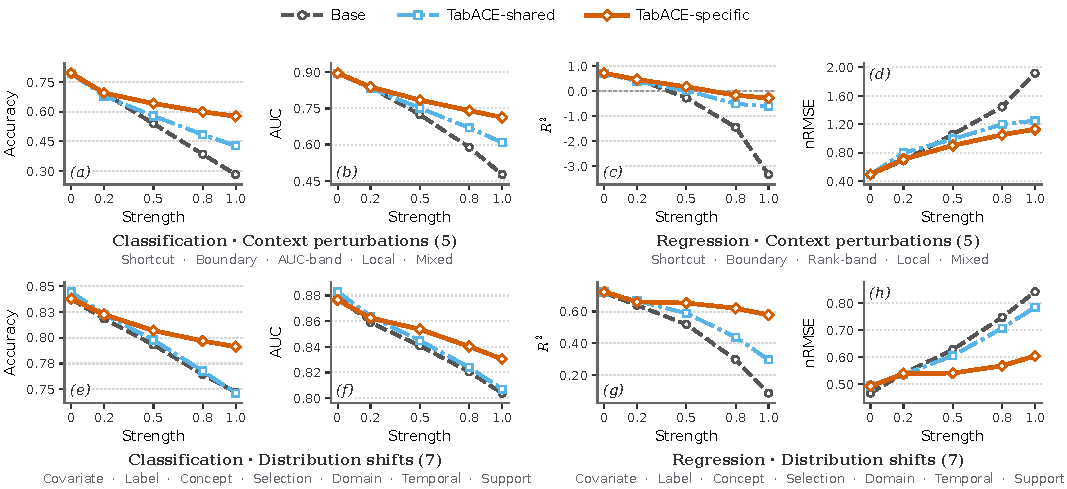
\includegraphics[width=\textwidth]{figures/tabace_limix_2m_strength_summary.pdf}
  \caption{LimiX-2M 在不同偏移强度下的结果。各行分别汇总五种上下文扰动与七种分布偏移；各列报告 Accuracy、AUC、$R^2$ 和 nRMSE（越低越好）。}
  \label{fig:limix-strength-summary}
\end{figure}

\begin{figure}[H]
  \centering
  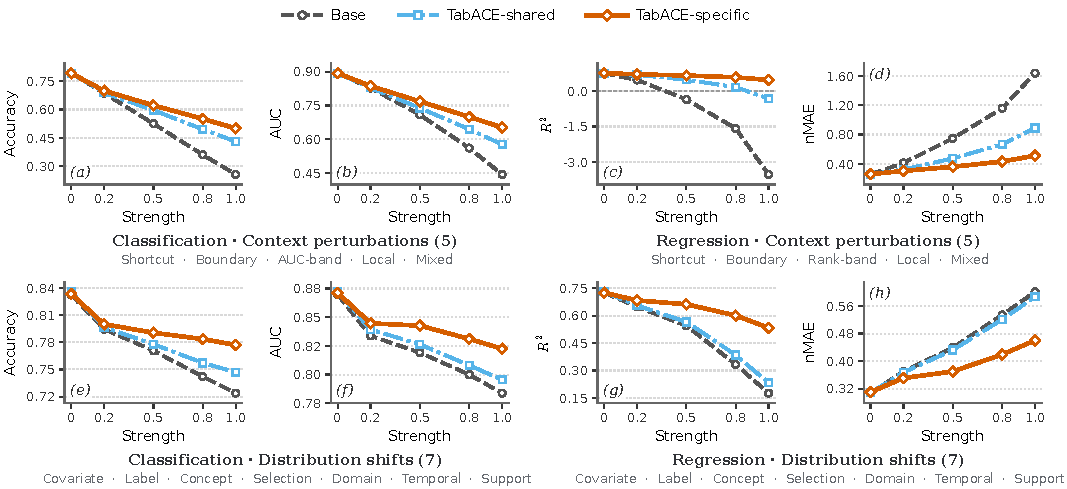
\includegraphics[width=\textwidth]{figures/tabace_tabpfn_v3_strength_summary.pdf}
  \caption{TabPFN-v3 在不同偏移强度下的结果。各行分别汇总五种上下文扰动与七种分布偏移；各列报告 Accuracy、AUC、$R^2$ 和 nMAE（越低越好）。}
  \label{fig:tabpfn-strength-summary}
\end{figure}

\begin{figure}[H]
  \centering
  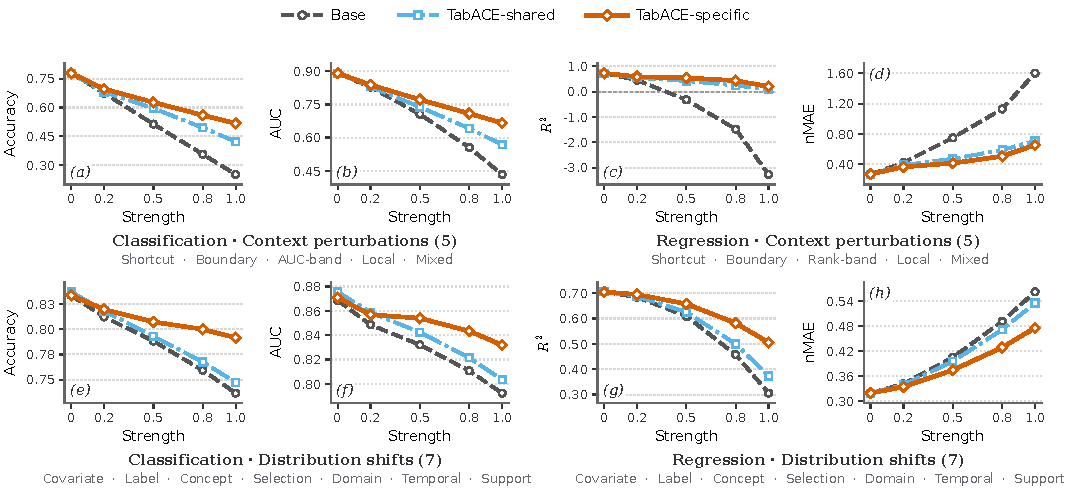
\includegraphics[width=\textwidth]{figures/tabace_tabdpt_v1_2_strength_summary.pdf}
  \caption{TabDPT v1.2 在不同偏移强度下的结果。各行分别汇总五种上下文扰动与七种分布偏移；各列报告 Accuracy、AUC、$R^2$ 和 nMAE（越低越好）。}
  \label{fig:tabdpt-strength-summary}
\end{figure}

\FloatBarrier
\vspace{-0.5em}
\section{消融研究}
\label{app:supplemental_ablations}

采用一个五上下文共享参考上下文库，选择在每个外部培训折叠。上下文预算研究评估嵌套的预先语，而剩余的研究保持所有五上下文固定。这种设计将上下文数量，聚合和公式组件的影响从上下文重新选择中隔离.

\subsection{上下文预算}
\label{app:context-budget}

我们的背景预算从$R=1$为了$R=5$单文本设置的基础，之后所有六个指标都变得单调和$R=5$总体超过Base. 这一趋势与第2节的补充性分析一致.~\ref{sec:theory}其他相关问题: 添加的文本可以涵盖以前未修复的查询.

\begin{figure}[H]
  \centering
  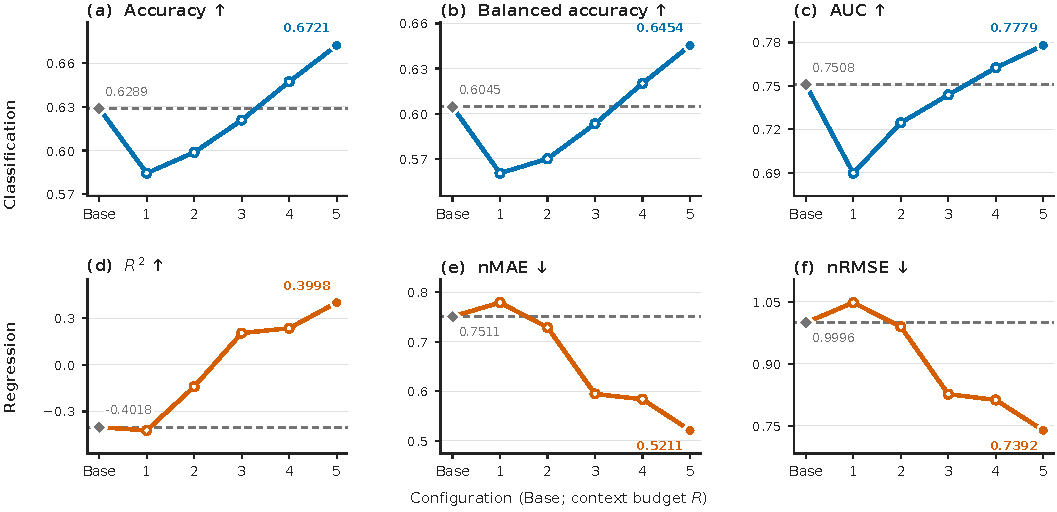
\includegraphics[width=\textwidth]{figures/tabace_context_count_ablation.pdf}
  \caption{根据本文数值，每一个曲线从Base开始，继续通过$R=1,\ldots,5$五个乱和七个转换轨道获得相同的宏观权重。只有少数背景下，转换覆盖范围是有限的。随着补充的背景添加，性能会提高，并且
  $R=5$箭头指的是最喜欢的方向.}
  \label{fig:context-count}
\end{figure}

\vspace{-0.45em}
\subsection{聚合规则}
\label{app:aggregation-rule}

通过使用相同的五个上下文上下文库，我们将平均，中值，剪缩中值和外折重积分进行比较，同时保持上下文数量和成员数量固定。用于分类，在抛弃每个类的五个最大和最小值后，坐标中值和平均值被重新归一化为概率简体;回归将相同的运算符应用于规模预测。这些仅基于上下文的变体取代了整个聚合规则,
因此，没有使用 $Q_i$, $S_i$,或Base gate. 折叠式权重规则达到最高分类精度和最低回归率 nRMSE,显示了源学习可靠性权重对这个上下文库无权重统计汇总的好处.

\begin{figure}[H]
  \centering
  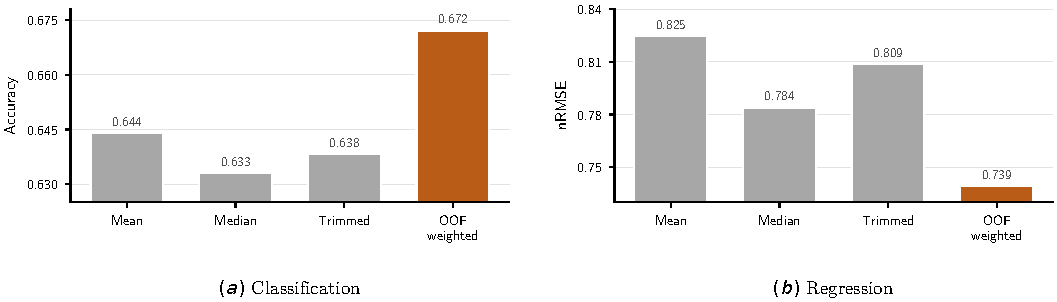
\includegraphics[width=\textwidth]{figures/tabace_aggregation_ablation.pdf}
  \caption{总结规则的减算$R=5$五和七的轨道均重。板组比较分类精度和回归 nRMSE.}
  \label{fig:aggregation-ablation}
\end{figure}

\vspace{-0.45em}
\subsection{固定上下文库组件消融}
\label{app:fixed-bank-formula-diagnostic}

在这种诊断配置中，我们将每个格特定的五个文本上下文库固定并一次删除一个组件。所有聚合和门控参数都在相应的外部训练格上选择，并且仅用于评估。我们评估了五个格:\emph{信心}组件$\eta_Q=0$保持$Q_i$在$E_i$;
\emph{协议}组件$\eta_S=0$; \emph{统一的牧师}组件$\pi_r=1/R$; \emph{/o 基门控}组件$U_i=1$; \emph{文本门控}
组件$E_i=1$. \emph{信心}适用于分类，其公式包括$Q_i$在五和七轨道中平均四个非零强度，然后给轨道提供相同的权重.

\begin{figure}[H]
  \centering
  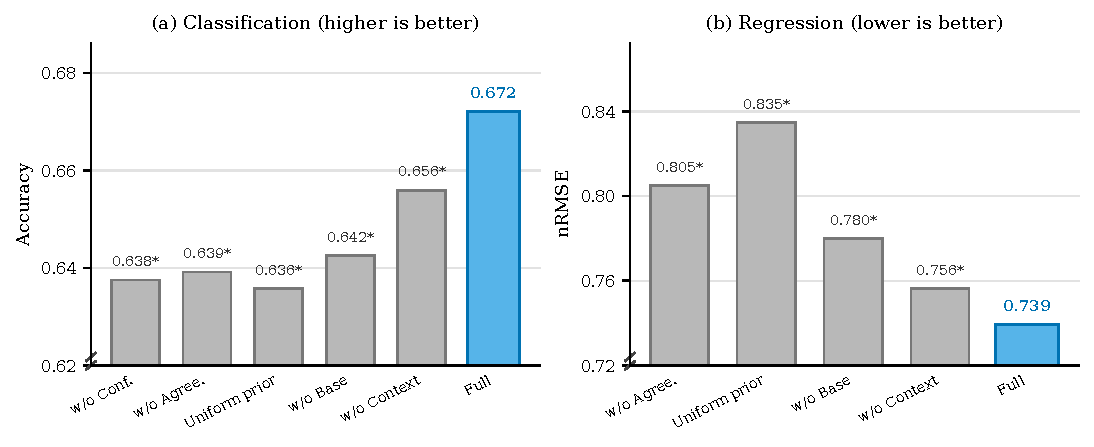
\includegraphics[width=\textwidth]{figures/tabace_k5_formula_diagnostic.pdf}
  \caption{组件的排序和回归。更高的精度和更低的 nRMSE 较好。灰色条除了一个组件的固定上下文库参考，显示的最后蓝色条。值在每个条以上打印，星标标记Holm-纠正的对配标志翻转$p<0.05$断裂标志表明截断的垂直轴.}
  \label{fig:k5-formula-diagnostic}
\end{figure}

固定上下文库参考达到0.672准确度和0.739nRMSE. 删除信心，协议，学习前，基础门控户或上下文门控户，将分别降低分类准确度至0.638,0.639,0.636,0.642,和0.656.
由于两项任务之前的学习环境而产生.

\subsection{不同证据分箱下的门控行为}
\label{app:gate-bin-analysis}

我们按任务分别将 752,144 个查询预测划分到 Base 不可靠性 $U_i$ 与上下文证据 $E_i$ 的三分位分箱中。每个单元格报告相对 Base 的平均插值权重与损失增益，以及实质性修改的比例（$\alpha_i\geq0.5$）及其恶化率。

\begin{figure}[H]
  \centering
  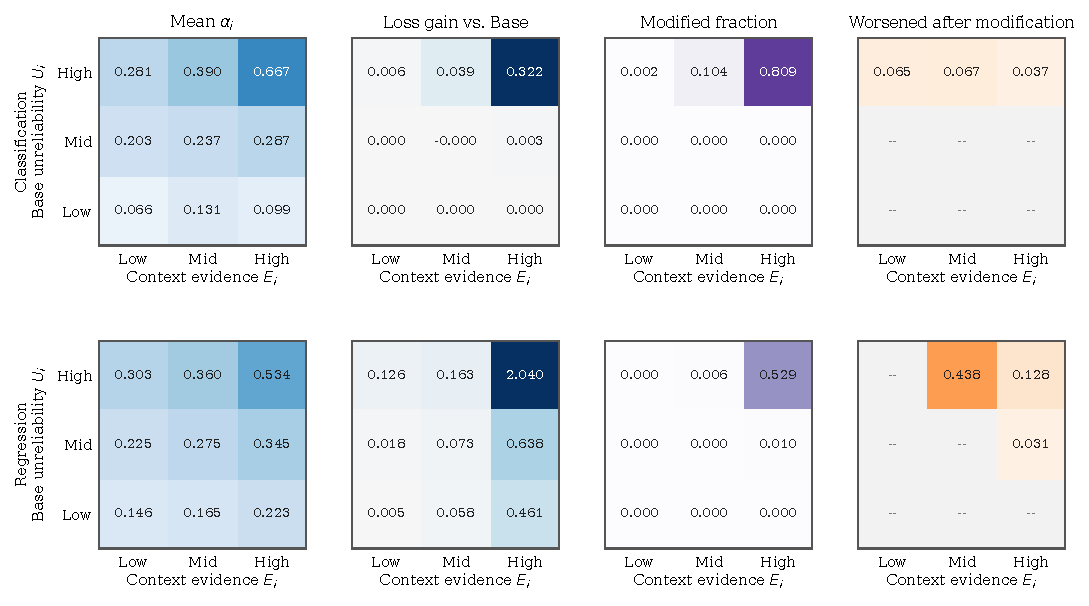
\includegraphics[width=0.68\textwidth]{figures/tabace_gate_bin_analysis.pdf}
  \caption{Base 不可靠性（$U_i$）与上下文证据（$E_i$）三分位分箱下的门控行为。正增益表示性能改善；灰色单元格没有实质性修改。在高 $U_i$/高 $E_i$ 分箱中，分类/回归的插值权重为 0.667/0.534，修改率为 0.809/0.529，损失增益为 0.322/2.040，恶化率为 0.037/0.128；低/低分箱的损失增益为 0.000/0.005。}
  \label{fig:gate-bin-analysis}
  \vspace{-0.5em}
\end{figure}

在回归的高 $U_i$/中 $E_i$ 单元格中，仅有 $0.6\%$ 的查询获得实质性更新；这些查询的条件恶化率为 $43.8\%$，而单元格层面的平均损失增益仍为正，为 $0.163$。

\FloatBarrier
\endgroup


\end{document}
